%                                     MMMMMMMMM        
%                                                                             
%  MMO    MM   MMMMMM  MMMMMMM   MM    MMMMMMMM   MMD   MM  MMMMMMM MMMMMMM   
%  MMM   MMM   MM        MM     ?MMM              MMM$  MM  MM         MM     
%  MMMM 7MMM   MM        MM     MM8M    MMMMMMM   MMMMD MM  MM         MM     
%  MM MMMMMM   MMMMMM    MM    MM  MM             MM MMDMM  MMMMMM     MM     
%  MM  MM MM   MM        MM    MMMMMM             MM  MMMM  MM         MM     
%  MM     MM   MMMMMM    MM   MM    MM            MM   MMM  MMMMMMM    MM
%
%
%            - META-NET Language White Paper | Irish content -
% 
% ----------------------------------------------------------------------------

\begin{document}

\maketitle

% --------------------------------------------------------------------------
\bsection*{Réamhrá --- Preface} 

\null
\pagestyle{empty} 

\pagenumbering{Roman} 
\setcounter{page}{5}
\pagestyle{scrheadings}

%\cleardoublepage

\begin{Parallel}[c]{78mm}{78mm}
\ParallelLText{\selectlanguage{irish}
Tá an páipéar bán seo mar chuid de shraith a chuireann chun cinn faisnéis maidir le teicneolaíocht teanga agus a cumas. Díríonn sé ar oideachasóirí, iriseoirí, polaiteoirí, pobail teanga agus daoine eile. 

Tá difríochtaí idir infhaighteacht agus úsáid teicneolaíocht teanga san Eoraip ó theanga go teanga. Dá bhrí sin, ní hionann na gníomhaíochtaí a theastaíonn chun tuilleadh tacaíochta a thabhairt do thaighde agus forbairt teicneolaíochtaí teanga i ngach teanga. Braitheann na gníomhaíochtaí a theastaíonn ar go leor tosca, cosúil le castacht na teanga agus méid a pobail.

Tá anailís déanta ag META-NET, Gréasán Sármhaitheasa arna mhaoiniú ag Coimisiún na hEorpa, ar na hacmhainní agus teicneolaíochtaí teanga reatha (lch.~\pageref{whitepaperseries}). Dhírigh an anailís seo ar na 23 teanga oifigiúil Eorpach mar aon le teangacha náisiúnta agus réigiúnacha tábhachtacha eile san Eoraip. Tugann torthaí na hanailíse seo le fios go bhfuil bearnaí taighde suntasacha i ngach teanga. Cuideoidh anailís agus measúnú saineolach níos mionsonraithe ar an gcás reatha le tionchar taighde bhreise a uasmhéadú agus na rioscaí a íoslaghdú.

Tá 54 ionad taighde as 33 tír i META-NET atá ag oibriú le geallsealbhóirí ó ghnólachtaí tráchtála (p.~\pageref{metanetmembers}), gníomhaireachtaí rialtais, tionscal, eagraíochtaí taighde, cuideachtaí bogearraí, soláthraithe teicneolaíochta agus ollscoileanna san Eoraip. Le chéile, tá siad ag cruthú comhfhís teicneolaíochta agus ag forbairt clár taighde straitéiseach a léiríonn an chaoi gur féidir le feidhmchláir teicneolaíochta teanga dul i ngleic le bearna i dtaighde faoi 2020.}

\ParallelRText{\selectlanguage{english}
This white paper is part of a series that promotes knowledge about language technology and its potential. It addresses journalists, politicians, language communities, educators and others. 
The availability and use of language technology in Europe varies between languages. Consequently, the actions that are required to further support research and development of language technologies also differ. The required actions depend on many factors, such as the complexity of a given language and the size of its community.

META-NET, a Network of Excellence funded by the European Commission, has conducted an  analysis of current language resources and technologies in this white paper series (p.~\pageref{whitepaperseries}). The analysis focuses on the 23 official European languages as well as other important national and regional languages in Europe. The results of this analysis suggest that there are tremendous deficits in technology support and significant research gaps for each language. The given detailed expert analysis and assessment of the current situation will help maximise the impact of future research.

As of November 2011, META-NET consists of 54 research centres in 33 European countries (p.~\pageref{metanetmembers}). META-NET is working with stakeholders from economy (software companies, technology providers and users), government agencies, research organisations, non-governmental organisations, language communities and European universities. Together with these communities, META-NET is creating a common technology vision and strategic research agenda for multilingual Europe 2020.}
\ParallelPar
\end{Parallel}

\makefundingnotice

% --------------------------------------------------------------------------

\cleardoublepage

\bsection*{Clár Ábhar --- Table of Contents}

\tableofcontents

\addtocontents{toc}{\protect\thispagestyle{empty}\protect}
\addtocontents{toc}{{\Large\textsf{\centerline{An GHAEILGE SA RÉ DHIGITEACH}}\par}} %NEED TO TRANSLATE

% --------------------------------------------------------------------------

\cleardoublepage

\setcounter{page}{1}
\pagenumbering{arabic} 
\pagestyle{scrheadings}

\ssection[Achoimre Fheidhmeach]{Achoimre Fheidhmeach}

\selectlanguage{irish}

\begin{multicols}{2}
Le 60 bliain anuas, tá an Eoraip tagtha chun cinn amhail struchtúr polaitiúil agus eacnamaíoch, ach tá éagsúlacht mhór fós inti maidir le cultúr agus teangacha. Dá bhrí sin, ón bPortaingéilis go Polainnis agus ó Iodáilis go hÍoslainnis, bíonn baic theanga i gceist le cumarsáid laethúil idir saoránaigh na hEorpa mar aon le cumarsáid sa saol gnó agus polaitiúil. Caitheann institiúidí an AE timpeall billiún euro sa bhliain ar a mbeartas ilteangachais a chothabháil, i.e. aistriú téacsanna agus teangaireacht a dhéanamh ar chumarsáid labhartha. An gá gur ualach chomh mór a bheadh anseo? Tig le teicneolaíocht teanga (TT) nua-aimseartha agus taighde theangeolaíoch cabhrú leis na teorainneacha teangeolaíocha a shárú. Nuair a nasctar an teicneolaíocht teanga le gairis agus feidhmchláir chliste, beidh sí in ann amach anseo cuidiú le muintir na hEorpa labhairt go héasca lena chéile agus gnó a dhéanamh lena chéile, fiú mura labhraíonn siad an teanga chéanna.  

\boxtext{Cruthaíonn teicneolaíocht teanga droichid do thodhchaí na hEorpa.}

Baineann geilleagar na hÉireann an-bhuntáiste as an margadh Eorpach aonair: 

In 2010, b’ionann trádáil san AE agus 57.9\% d’easpórtálacha na hÉireann agus b’ionann trádáil le tíortha Eorpacha eile agus 4.9\% \cite{csoirishtrade}.
Ach tig le baic theanga stop a chur le gnó, go háirithe le SMEanna nach bhfuil na hacmhainní airgeadais acu an cás a chur ina cheart.
An t-aon rogha (tubaisteach) a bheadh ann ar an Eoraip ilteangach seo go mbeadh teanga amháin ceannasach agus go dtiocfadh sí in áit na dteangacha eile.

Bealach amháin chun bac teanga a shárú is ea teangacha iasachta a fhoghlaim. Ach gan tacaíocht theicneolaíoch, ní fhéadfadh saoránaigh na hEorpa agus a geilleagar, díospóireacht pholaitiúil agus dul chun cinn eolaíochta máistreacht a fháil ar na 23 teanga oifigiúil agus na 60 eile teanga Eorpach. 

Is é réiteach na faidhbe príomhtheicneolaíochtaí cumasaithe a thógáil. Gheobhaidh rannpháirtithe Eorpacha buntáistí ollmhóra astu seo, ní hamháin sa chómhargadh Eorpach agus i gcaidreamh trádála le geilleagair forbarthacha, go háirithe le geilleagair éiritheacha.  Chun an sprioc seo a bhaint amach agus éagsúlacht chultúir agus theangeolaíoch na hEorpa a chaomhnú, is gá ar dtús anailís chórasach a dhéanamh ar mhionsonraíochtaí teanga na dteangacha Eorpacha ar fad, agus an bhail reatha atá ar thacaíocht teicneolaíochta dóibh. Beidh réitigh teicneolaíochta teanga ina ndroichid uathúla idir teangacha Eorpacha faoi dheireadh.  

\boxtext{Teicneolaíocht teanga ina heochair don todhchaí.}

Ní shásaíonn na huirlisí aistriúcháin uathoibríocha agus próiseála urlabhra atá ar an margadh faoi láthair an sprioc uaillmhianach seo. Tá na rannpháirtithe ceannasacha sa réimse seo faoi úinéireacht phríobháideach go príomha chun brabach a dhéanamh agus bunaithe i Meiriceá Thuaidh. Bhí a fhios ag an AE faoi dheireadh na 1970idí go raibh teicneolaíocht teanga an\-ábhartha mar thiománaí d’aontacht Eorpach, agus chuir siad tús leis na chéad tionscadail taighde, amhail EUROTRA. Ag an am céanna, bunaíodh go leor tionscadail náisiúnta a chothaigh torthaí luachmhara, ach nár eascair gníomhaíocht Eorpach astu. I gcodarsnacht leis an iarracht mhaoinithe ardroghnach seo, bhunaigh sochaithe ilteangacha eile cosúil leis an India (22 teanga oifigiúil) agus an Afraic Theas (11 theanga oifigiúla) cláir náisiúnta fhadtéarmacha do thaighde agus forbairt teicneolaíochta teanga. 

Tá na gníomhairí is mó i dteicneolaíocht teanga inniu ag brath ar chur chuige staitistiúil neamhbheacht nach n-úsáideann modhanna agus faisnéis theangeolaíoch níos doimhne. Mar shampla, aistrítear abairtí go huathoibríoch trí abairt nua a chur i gcomparáid leis na mílte abairt a d’aistrigh daoine cheana. Braitheann caighdeán an aschuir go mór ar mhéid agus caighdeán an chorpais shamplaigh atá ar fáil. Cé gur féidir torthaí sásúla a fháil as aistriú uathoibríoch abairtí simplí i dteangacha ina bhfuil dóthain ábhair théacs ar fáil, ní éireoidh le modhanna staitistiúla chomh héadomhain sin i gcás teangacha ina bhfuil corpas ábhar téacs i bhfad níos lú nó i gcás abairtí le struchtúir chasta.

Dá bhrí sin, tá cinneadh déanta ag an Aontas Eorpach maoniú a thabhairt do thionscadail cosúil le EuroMatrix agus EuroMatrixPlus (ó 2006) agus iTranslate4 (ó 2010) a dhéanann taighde bunúsach agus feidhmeach agus a chothaíonn acmhainní chun réitigh theicneolaíochta teanga ardchaighdeáin a bhunú do gach teanga Eorpach. Is é an t-aon bhealach chun dul chun cinn a dhéanamh anailís a dhéanamh ar airí struchtúrtha níos doimhne teangacha má theastaíonn uainn feidhmchláir a thógáil a fheidhmíonn go maith don réimse teangacha ar fad san Eoraip.

Tá rath bainte amach ag taighde Eorpach sa réimse seo cheana. Mar shampla, úsáidtear MOSES, bogearra aistriúcháin uathoibríoch foinse oscailte, a forbraíodh go príomha trí thionscadail taighde Eorpacha anois i seirbhísí aistriúcháin an Aontais Eorpaigh. Chuir tionscadal Verbmobil, arna mhaoiniú ag Aireacht Oideachais agus Taighde na Gearmáine (BMBF) idir 1993 agus 2000, an Ghearmáin chun tosaigh i réimse an taighde um aistriú urlabhra ar feadh scathaimh. Dúnadh nó bogadh chuig ionad eile go leor de na saotharlanna taighde agus forbartha a bhí sa Ghearmáin ag an am (e.g. IBM agus Philips). In ionad dul ar aghaidh ó thorthaí na dtionscadal taighde seo, dhírigh an Eoraip ar ghníomhaíochtaí taighde aonair nach raibh tionchar chomh forleatach acu ar an margadh.  Is féidir luach geilleagrach na n-iarrachtaí is luaithe fiú a fheiceáil sa líon seachthionscadal. Díoladh an chuideachta Trados, a bunaíodh i 1984, le SDL atá bunaithe sa RA in 2005.


\boxtext{Cuidíonn Teicneolaíocht Teanga chun an Eoraip a chomhaontú.}

Ag tarraingt ar an léargas a fuarthas go dtí seo, is léir go mbeidh teicneolaíocht teanga ‘hibride’ an lae inniu, a mheascann próiseáil dhomhain le modhanna staitistiúla, in ann an bhearna idir gach teanga Eorpach agus teangacha eile nach iad a líonadh. Mar a léirítear sa tsraith páipéar bána seo, tá difríocht ollmhór sa staid ullmhachta maidir le réitigh theanga agus an staid taighde idir ballstáit na hEorpa. Tá an Ghaeilge, mionteanga san AE, agus go deimhin in Éirinn, i mbaol bheith fágtha taobh thiar i ndáil le dul chun cinn mura ngníomhaítear i dtreo bunteicneolaíocht teanga comhpháirte a sholáthar le tacú leis an teanga. Ag an am céanna, tá Éire i staid láidir chun na teicneolaíochtaí seo a fhorbairt agus ról lárnach bheith aici go geilleagrach agus i dtaobh na heolaíochta i ndul chun cinn suntasach a dhéanamh sa réimse ina iomláine, de bharr ardchaighdeán in aistriúchán agus logánú agus taighde teicneolaíocht teanga. 

Is í sprioc fhadtéarmach META-NET teicneolaíocht teanga ardchaighdeáin a chur ar fáil do gach teanga d’fhonn comhaontacht pholaitiúil agus gheilleagrach a bhaint amach trí éagsúlacht chultúrtha. Cuideoidh an teicneolaíocht le baic reatha a bhaint anuas agus droichid a chruthú idir teangacha na hEorpa. Chun é seo a bhaint amach, caithfidh gach geallsealbhóir – polaitíochta, taighde, gnó agus sochaí – a n-iarrachtaí a chur le chéile sa todhchaí.

Cuireann an tsraith páipéar bán seo le gníomhaíochtaí straitéiseacha eile a rinneadh META-NET (feic an aguisín chun léargas ginearálta a fháil). Is féidir faisnéis suas chun dáta cosúil le leagan reatha an pháipéir fhíse META-NET \cite{Meta1} nó Clár Taighde Straitéiseach (SRA) a fháil ar shuíomh gréasáin META-NET:  http://www.meta-net.eu

\end{multicols}

\clearpage

% --------------------------------------------------------------------------

\ssection[Riosca dár dTeangacha agus Dúshlán dár dTeicneolaíocht Teanga]{Riosca dár dTeangacha agus Dúshlán dár dTeicneolaíocht Teanga}

\begin{multicols}{2}

Táimid i lár réabhlóid dhigiteach a bhfuil tionchar suntasach aici ar chumarsáid agus ar an tsochaí. Cuirtear forbairtí a rinneadh le déanaí i dteicneolaíocht fainséise agus chumarsáide digití i gcomparáid uaireanta le hairgeadh Gutenberg an chlóphreasa. Céard a insíonn an analach seo dúinn faoi thodhchaí shocaí faisnéise na hEorpa agus ár dteangacha go háirithe?

\boxtext{I láthair na huaire tá réabhlóid dhigiteach ar siúl ar féidir í a chur i gcomparáid le hairgeadh Gutenberg an chlóphreasa.}

Tar éis airgeadh Gutenberg, baineadh amach dul chun cinn suntasach i gcumarsáid agus malartú faisnéise trí iarrachtaí cosúil le haistriú Luther ar an mBíobla i dteanga logánta. Sna haoiseanna ina dhiaidh sin, forbraíodh teicníochtaí cultúrtha chun próiseáil teanga agus malartú faisnéise a láimhseáil ar bhealach níos fearr:

\medskip
\begin{itemize}
\item chumasaigh caighdeánú ortagrafach agus gramadaí na mórtheangacha scaipeadh tapa smaointe eolaíocha agus intleachta nua;
\item chuir forbairt teangacha oifigiúla ar chumas saoránaigh cumarsáid a dhéanamh laistigh de theorainneacha éagsúla (teorainneacha polaitiúla go minic);
\item chumasaigh múineadh agus aistriú teangacha malartuithe thar theangacha;
\item chinntigh cruthú treoirlínte eagarthóireachta agus bibleagrafacha caighdeán agus infhaighteacht ábhar priontailte;
\medskip
\item shásaigh cruthú meán éagsúla cosúil le nuachtáin, raidió, teilifís, leabhair agus formáidí eile riachtanais éagsúla chumarsáide.
\end{itemize}

Le fiche bliain anuas, tá teicneolaíocht fasnéise ag cuidiú le go leor próiseas a uathoibriú agus a éascú:

\begin{itemize}
\item tá bogearraí um fhoilsitheoireacht deisce tagtha in ionad clóscríofa agus clóchuir;
\item tá Microsoft PowerPoint tagtha in ionad leathanaigh thrédhearcacha ar osteilgeoir;
\item seolann agus faigheann ríomhphoist cáipéisí níos tapúla ná meaisín facsála;
\item is féidir glaonna Idirlín saora agus cruinnithe fíorúla a reáchtáil le Skype;.
\item is éasca ábhar ilmheáin a mhalartú i bhformáidí ionchódaithe fuaime agus físe;
\item tugann innill chuardaigh rochtain ar leathanaigh ghréasain bunaithe ar eochairfhocail;
\item tugann seirbhísí cosúil le Google Translate neasaistriúcháin ghasta;
\item éascaíonn léibhinn mheáin shóisialta amhail Facebook, Twitter agus Google+ cumarsáid, comhoibriú agus roinnt faisnéise.
\end{itemize}

Cé go bhfuil uirlisí agus feidhmchláir mar seo úsáideach, níl siad in ann tacú le sochaí inbhuanaithe, ilteangach na hEorpa do chách go fóill, inar féidir le faisnéis agus earraí sreabhadh go héasca.

\subsection{Cuireann Teorainneacha Teanga Bac ar Shochaí Faisnéise na hEorpa}
  
Ní thig linn a thuar cén chuma a bheidh ar an tsochaí faisnéise amach anseo. Ach tá seans láidir ann go bhfuil an reábhlóid i dteicneolaíocht chumarsáide ag tabhairt daoine a labhraíonn teangacha difriúla le chéile ar bhealaí nua. Tá brú á chur aige seo ar dhaoine teangacha nua a fhoghlaim agus go háirithe ar fhorbróirí chun feidhmchláir theicneolaíochta nua a chruthú a chinnteoidh comhthuiscint agus rochtain ar fhaisnéis is féidir a roinnt. I spás geilleagrach agus faisnéise domhanda, déanann níos mó teangacha, cainteoirí agus ábhar idirghníomhaíocht níos tapúla le cineálacha nua meán. Níl san éileamh mór atá ar mheáin shóisialta faoi láthair (Wikipedia, Facebook, Twitter, YouTube agus le déanaí, Google+) ach tús an scéil.

\boxtext{Tá geilleagar domhanda agus spás faisnéise ag cur níos mó teangacha, cainteoirí agus ábhar os ár gcomhair.}

Inniu, tig linn téacs gigibhearta a sheoladh ar fud an domhain i soicindí sula mbíonn a fhios againn go bhfuil sé i dteanga nach dtuigimid. De réir tuarascáil nua ó Choimisiúin na hEorpa, ceannaíonn 57\% d ‘úsáideoirí an Idirlín san Eorpaip earraí agus seirbhísí i dteangacha nach iad a dteanga dhúchais iad. (Is é an Béarla an teanga iasachta is coitianta, agus ansin an Fhraincis, an Ghearmáinis agus an Spáinnis.) Léann 55\% d'úsáideoirí ábhar i dteanga iasachta cé nach n-úsáideann ach 35\% teanga eile chun teachtaireachtaí a scríobh nó nótaí tráchtaireachta a fhágáil ar an ngréasán \cite{EC1}.  Roinnt blianta ó shin, ba é an Béarla francbhéarla an ghréasáin -– bhí formhór an ábhair ar an ngréasán i mBéarla – ach tá athrú ollmhór tagtha ar chúrsaí anois. Tá méadú as cuimse tagtha ar ábhar ar líne i dteangacha eile na hEorpa (mar aon le teangacha Áiseacha agus ón Meánoirthear).

Níl mórán aird phoiblí faighte ag an deighilt dhigiteach uileláithreach seo; cé go n-ardaíonn sé ceist an-tábhachtach: Cé na teangacha Eorpacha a bheidh faoi bhláth sa tsochaí faisnéise agus eolais ghréasánaithe, agus cé acu a imeoidh i léig?

\subsection{Ár dTeangacha i mBaol}

Cé gur chuidigh an clóphreas le malartú faisnéise san Eoraip a fheabhsú, chuaigh roinnt teangacha Eorpacha in éag mar gheall air chomh maith. B’annamh a cuireadh teangacha réigiúnacha ná mionlacha i gcló agus bhí teangacha amhail Coirnis agus Dalmáitis teoranta do chineálacha aistrithe béil, a chur teorainn lena scóp úsáidte. An mbeidh an tionchar céanna ag an Idirlíon ar ár dteangacha?

Tá timpeall 80 teanga na hEorpa ar cheann dá sócmhainní cultúrtha is saibhre agus is tábhachtaí agus mar chuid lárnach dá mhúnla sóisialta \cite{EC2}.  Cé gur dóchúil go mairfidh teangacha amhail an Béarla agus an Spáinnis san áit mhargaidh dhigitigh nua, d’fhéadfadh teangacha Eorpacha bheith mí\-ábhartha i sochaí ghréasánaithe. Lagódh sé seo seasamh domhanda na hEorpa, agus théadh sé in aghaidh na sprice straitéisí de rannpháirtíocht chothrom a chinntiú do gach saoránach Eorpach beag beann ar theanga.  


\boxtext{Tá an réimse leathan teangacha san Eoraip ar cheann dá sócmhainní cultúrtha is saibhre agus is tábhachtaí.}

De réir thuarascáil UNESCO ar ilteangachas, is meán ríthábhachtach iad teangacha chun bunchearta a fháil, cosúil le léiriú polaitiúil, oideachas agus rannpháirtíocht i sochaí \cite{Unesco1}.

\subsection{Is Teicneolaíocht Chumasaithe atá i dTeicneolaíocht Teanga}

San am a caitheadh, dhírigh iarrachtaí infheistíochta i gcaomhnú teanga ar oideachas agus aistriú teanga. De réir meastachán amháin, b’ionann an margadh Eorpach d’aistriúchán, teangaireacht, bogearraí logánaithe agus domhandú suíomhanna gréasáin agus \texteuro 8.4 billiún in 2008 agus táthar ag súil go bhfásfaidh sé 10\% sa bhliain \cite{EC3}.  Ach ní chlúdaíonn an figiúr seo ach cuid bheag de riachtanais reatha agus amach anseo na cumarsáide idir teangacha. Is é an réiteach is fearr atá ar fáil chun leithead agus doimhneacht úsáid teanga a chinntiú san Eoraip sa todhchaí an teicneolaíocht chuí a úsáid, díreach mar a úsáidimid teicneolaíocht chun ár riachtanais iompair, fuinnimh agus míchumais i measc nithe eile a réiteach.

Cuidíonn teicneolaíocht teanga dhigiteach (ag díriú ar gach cineál téacs scríofa agus dioscúrsa labhartha) le daoine comhoibriú, gnó a dhéanamh, faisnéis a roinnt agus bheith rannpháirteach i ndíospóireacht shóisialta agus pholaitiúil in ainneoin baic theanga agus scileanna ríomhaireachta. Feidhmíonn sé go minic laistigh de chórais bhogearraí choimpléascacha le cuidiú linn:

\begin{itemize}
\item faisnéis a fháil le hinneall cuairdaigh Idirlín;
\item litriú agus gramadach a sheiceáil i bpróiseálaí focal;
\item féachaint ar mholtaí táirge i siopa ar líne;
\item treoracha ó bhéal a chloisteáil ó chóras treoshuímh chairr;
\item leathanaigh ghréasáin a aistriú trí sheirbhís ar líne. 
\end{itemize}

Tá roinnt príomh-fheidhmchlár i dteicneolaíocht teanga a chumasaíonn próisis laistigh de chreat feidhmchláir níos mó. Is í aidhm pháipéar bán theanga META-NET díriú ar chomh réidh is atá na croítheicneolaíochtaí seo do gach teanga Eorpach.  

\boxtext{Teastaíonn teicneolaíocht teanga láidir agus inacmhainne don Eoraip do gach teanga Eorpach.}

Chun ár staid a chothabháil ar thúslíne na nuálaíochta domhanda, beidh teicneolaíocht teanga de dhíth ar an Eoraip a bheidh in oiriúint do gach teanga Eorpach atá laidir, inacmhainne agus comhtháite go daingean i dtimpeallachtaí bogearraí tábhachtacha. Gan teicneolaíocht teanga, ní bheimid in ann taithí úsáideora idirghníomhach, ilmheáin agus ilteanga atá an-éifeachtach a bhaint amach sna blianta atá romhainn.

\subsection{Deiseanna do Theicneolaíocht Teanga}

I ndomhan na priontála, ba é an t-iontas teicneolaíochta an dúbailt ghasta d'íomhá théacs (leathanach) agus clóphreas oiriúnach á úsáid. B’éigean do dhaoine an obair chrua a dhéanamh, cuardach, léamh, aistriú agus achoimre a thabhairt ar fhaisnéis. B’éigean dúinn fanacht go dtí gur thaifead Edison an teanga labhartha -– agus arís go dtí go ndearna a theicneolaíocht cóipeanna analóige.

Tig le teicneolaíocht teanga dhigiteach anois uathoibriú a dhéanamh ar na próisis aistrithe, táirgthe ábhar, agus bainistithe faisnéise do gach teanga Eorpach. Tig leis chomh maith cumhacht a thabhairt do chomhéadain teanga/urlabhra do leictreonaigh, innill, feithiclí, ríomhairí agus róbait tí. Tá feidhmchláir fhíora thráchtála agus thionscail fós sna céimeanna luatha forbartha, ach tá deis iontach á cruthú ag gnóthachtálacha taighde agus forbartha. Mar shampla, tá aistriúchán uathoibríoch réasúnta cruinn i bhfearainn ar leith, agus cuireann feidhmchláir thrialacha faisnéis ilteangach agus bainistiú faisnéise ar fáil mar aon le táirgeadh ábhair in go leor teangacha Eorpacha. 

Mar aon le formhór teicneolaíochtaí, forbraíodh na chéad feidhmchláir theanga cosúil le comhéadain ghlórbhunaithe agus córais dialóige d’fhearainn ardspeisialaithe, agus go minic ní bhíonn ach feidhmíocht theoranta acu. Ach tá deiseanna margaidh iontacha sna tionscail oideachais agus siamsaíochta chun teicneolaíochtaí teanga a chomhtháthú i gcluichí, suíomhanna oidhreachta cultúrtha, pacáistí oideachas-siamsaíochta, leabharlanna, timpeallachtaí ionsamhlaithe agus cláir oiliúna. I measc na bhfeidhmchlár ina bhfuil ról tábhachtach ag teicneolaíocht teanga tá seirbhísí faisnéise soghluaiste, bogearraí um fhoghlaim teanga ríomhchuidithe, timpeallachtaí ríomhfhoghlama, uirlisí féinmheasúnaithe agus bogearraí um brath bradaíola. Tugtar le fios ón éileamh mór atá ar fheidhmchláir mheáin sóisialta cosúil le Twitter agus Facebook go bhfuil tuilleadh gá le teicneolaíochtaí teanga sofaisticiúla ar féidir leo monatóireacht a dhéanamh ar phostálacha, achoimriú a dhéanamh ar phléití, treochtaí tuairime a mholadh, freagraí mothúchánacha a bhrath, sáruithe cóipchirt a bhrath nó mí-úsáid a aimsiú.

Tugann teicneolaíocht teanga deis iontach don Aontas Eorpach. Tig léi cabhrú le dul i ngleic le saincheist choimpléascach an ilteangachais san Eoraip – teangacha éagsúla bheith i láthair go nádúrtha i ngnólachtaí, eagraíochtaí agus scoileanna san Eoraip. Ach teastaíonn ó shaoránaigh cumarsáid a dhéanamh thar na teorainneacha teanga seo fud fad Mhargadh an Choimisiúin Eorpaigh, agus tig le teicneolaíocht teanga cuidiú leis an mbac seo a shárú trí thacú le húsáid shaor agus oscailte na dteangacha aonair. Ag breathnú níos faide chun tosaigh, cuirfidh teicneolaíocht teanga ilteangach tagarmharc ar fáil dár bpáirtithe domhanda nuair a thosóidh siad ag cumasú a bpobail ilteangacha féin. Is féidir breathnú ar theicneolaíocht teanga amhail teicneolaíocht ‘chúnta’ a chuidíonn leat `míchumas’ na héagsúlachta teanga a shárú agus pobail teanga bheith níos inrochtana dá chéile.

\boxtext{Cuidíonn teicneolaíocht teanga ``míchumas'' na héagsúlachta teangeolaíche a shárú.} 

Tugann teicneolaíocht teanga deis iontach don Aontas Eorpach. Tig léi cabhrú le dul i ngleic le saincheist choimpléascach an ilteangachais san Eoraip – teangacha éagsúla bheith i láthair go nádúrtha i ngnólachtaí, eagraíochtaí agus scoileanna san Eoraip. Ach teastaíonn ó shaoránaigh cumarsáid a dhéanamh thar na teorainneacha teanga seo fud fad Mhargadh an Choimisiúin Eorpaigh, agus tig le teicneolaíocht teanga cuidiú leis an mbac seo a shárú trí thacú le húsáid shaor agus oscailte na dteangacha aonair. Ag breathnú níos faide chun tosaigh, cuirfidh teicneolaíocht teanga ilteangach tagarmharc ar fáil dár bpáirtithe domhanda nuair a thosóidh siad ag cumasú a bpobail ilteangacha féin. Is féidir breathnú ar theicneolaíocht teanga amhail teicneolaíocht ‘chúnta’ a chuidíonn leat ‘míchumas’ na héagsúlachta teanga a shárú agus pobail teanga bheith níos inrochtana dá chéile.

Ar deireadh, réimse teanga gníomhach amháin is ea úsáid na teicneolaíochta teanga d’fheidhmíochtaí tarrthála i gceantair thubaiste, nuair a bhíonn beatha daoine i mbaol: Beidh sé de chumas ag róbait chliste amach anseo a bhfuil cumais teanga thrasteangacha acu beatha dhaoine a shábháil.

\subsection{Dúshláin le Teicneolaíocht Teanga}


Cé go bhfuil dul chun cinn mór déanta ag teicneolaíocht teanga le blianta beaga anuas, tá luas reatha an dul chun cinn teicneolaíochta agus nuálaíochta táirge rómhall. Is iondúil go mbíonn teicneolaíochtaí coitianta cosúil le ceartóirí litrithe agus gramadaí i bpróiseálaithe focail aonteangacha, agus níl siad ar fáil ach do líon beag teangacha. 

\boxtext{Tá dul chun cinn na teicneolaíochta rómhall faoi láthair.}

Tá deacrachtaí ag baint le seirbhísí uathaistriúcháin ar líne nuair atá aistriúcháin an-bheachta agus iomlána ag teastáil, cé go bhfuil siad úsáideach chun meastachán réasúnta a chur ar fáil d’ábhar cáipéisí. De bharr castacht teanga dhaonna, is gnó fada, costasach atá i dteangacha a mhúnlú i mbogearraí agus iad a thástáil sa saol dáiríre agus teastaíonn tiomantais mhaoinithe mharthanacha dó seo. Caithfidh an Eoraip, dá bhrí sin, a ról ceannródaíoch i ndul i ngleic le dúshláin teicneolaíochta a bhaineann le pobal ilteangach a chothabháil trí bhealaí nua a chruthú chun borradh a chur faoi fhorbairt ar fud na léarscála. D’fhéadfaí a áireamh anseo dul chun cinn ríomhaireachtúil agus teicníochtaí cosúil le sluafhoinsiú.


\subsection{Éadáil Teanga i nDaoine agus Innill}

Chun an chaoi a láimhseálann ríomhairí teanga a léiriú agus míniú a thabhairt ar an gcúis go bhfuil sé deacair iad a ríomhchlárú chun í a úsáid, feicimid go tapa ar an gcaoi a bhfaigheann daoine a gcéad agus dara teangacha, agus ansin feicimid an chaoi a n-oibríonn córais teicneolaíochta teanga.


\boxtext{Foghlaimíonn daoine scileanna teanga ar dhá bhealach éagsúla: ag foghlaim samplaí agus ag foghlaim rialacha teanga bunúsacha.}

Foghlaimíonn daoine scileanna teanga ar dhá bhealach éagsúla. Foghlaimíonn leanaí teanga trí bheith ag éisteacht le hidirchaidreamh idir tuismitheoirí, siblíní agus baill teaghlaigh eile. Ó aois dhá bhliain nó mar sin, labhraíonn leanaí a gcéad fhocail agus frásaí gearra. Is féidir é seo a dhéanamh mar tá claonadh géiniteach ag daoine na rudaí a chloiseann siad a aithris agus ansin réasúnú a dhéanamh air. 

Teastaíonn iarracht níos mó chun dara teanga a fhoghlaim agus tú níos sine, go príomha mar gheall nach bhfuil an leanbh tumtha i bpobal de chainteoirí dúchais. Ar an scoil, is iondúil go bhfoghlaimítear teangacha iasachta trí struchtúr gramadaí, stór focal agus litriú a fhoghlaim trí dhruileanna a úsáid a dhéanann cur síos ar fhaisnéis teanga i dtéarmaí rialacha teibí, táblaí agus samplaí. Bíonn sé níos deacra teanga iasachta a fhoghlaim nuair a bhíonn tú níos sine. 

`Foghlaimíonn' an dá phríomhchineál córas teicneolaíochta teanga cumais teanga ar bhealach cosúil leis sin. Faigheann cur chuige staitistiúil (nó ‘sonraíthiománta’) faisnéis teanga ó bhailiúcháin ollmhóra de théacsanna samplacha coincréite. Cé gur leor téacs aonair a úsáid i dteanga aonair d'oiliúint, e.g., seiceálaí litrithe, caithfidh téacsanna comhthreomhara in dhá theanga (nó níos mó) bheith ar fáil chun córas uathaistrithe a oiliúint. Ansin `foghlaimíonn' an t-algartam foghlama meaisín na pátrúin a bhaineann le focail, frásaí gearra agus abairtí iomlána a aistriú. 

D’fhéadfadh na milliún abairt bheith de dhíth don chur chuige staitistiúil seo agus ardaítear an fheidhmíocht de réir an lín téacsanna ar a ndéantar anailís. Is cúis amháin í seo go bhfuil fonn ar sholáthraithe innill chuardaigh a mhéid ábhar scríofa agus is féidir leo a bhailiú. Braitheann ceartú litrithe i bpróiseálaithe focal, agus seirbhísí cosúil le Cuardach Google agus Google Translate ar chur chuige staitistiúil. Is é an buntáiste is mó a bhaineann le staitisticí gur féidir leis an inneall foghlaim go tapa i sraith leanúnach timthrialacha oiliúna, cé gur féidir leis an gcaighdeán bheith an-éagsúil.

D’fhéadfadh na milliún abairt bheith de dhíth don chur chuige staitistiúil seo agus ardaítear an fheidhmíocht de réir an lín téacsanna ar a ndéantar anailís. Is cúis amháin í seo go bhfuil fonn ar sholáthraithe innill chuardaigh a mhéid ábhar scríofa agus is féidir leo a bhailiú. Braitheann ceartú litrithe i bpróiseálaithe focal, agus seirbhísí cosúil le Cuardach Google agus Gogle Translate ar chur chuige staitistiúil. Is é an buntáiste is mó a bhaineann le staitisticí gur féidir leis an inneall foghlaim go tapa i sraith leanúnach timthrialacha oiliúna, cé gur féidir leis an gcaighdeán bheith an-éagsúil. 

Mar gheall go mbíonn láidreachtaí agus laigí na gcóras staitistiúla agus riailbhunaithe comhlántach, díríonn taighde reatha ar chur chuige hibride a chuireann an dá mhodheolaíocht le chéile. Ach, níor éirigh chomh maith sin leis an gcur chuige sin go dtí seo i bhfeidhmchláir thionscail agus a d’éirigh leo sa tsaotharlann taighde. 

Mar a chonaiceamar sa chaibidil seo, braitheann go leor feidhmchlár a úsáidtear go fairsing i sochaí faisnéise an lae inniu ar theicneolaíocht teanga. De bharr a phobal ilteangach, is fíor é seo i spás geilleagrach agus faisnéise na hEorpa. Cé go bhfuil dul chun cinn mór déanta ag teicneolaíocht teanga le blianta beaga anuas, tá cumas mór ann go fóill chun caighdeán na gcóras teicneolaíochta teanga a fheabhsú. Anseo a leanas, déanfar cur síos ar ról na Gaeilge i sochaí faisnéise na hEorpa agus déanfar measúnú ar staid reatha na teicneolaíochta teanga don Ghaeilge.
\end{multicols}

\clearpage

% --------------------------------------------------------------------------

\ssection[An Ghaeilge i Sochaí Faisnéise na hEorpa]{An Ghaeilge i Sochaí Faisnéise na hEorpa}
\label{IrishInfso_ga}

\begin{multicols}{2}

\subsection{Fíricí Ginearálta}

Is teanga cheilteach í an Ghaeilge, a bhfuil gaol gairid aici le Gaeilge na hAlban, agus gaol níos faide amach leis an mBreatnais agus an mBriotáinis. Bhí sí á labhairt go forleathan go dtí lár an 18ú haois, tháinig meath tapa uirthi tar éis an Ghorta in Éirinn. Is teanga í an Ghaeilge, a labhraíonn 1,656,790 duine ag leibhéal áirithe, i bPoblacht na hÉireann (daonáireamh 2006) agus 167,490 duine i dTuaisceart Éireann (daonáireamh 2001) le pobail bheaga Ghaeilge lonnaithe timpeall an domhain i measc Dhiaspóra agus dhaoine acadúla na hÉireann, go háirithe sna Stáit Aontaithe, i gCeanada agus san Astráil. Is fórsa dearfach atá sa phobal domhanda seo, atá á éascú ag an ré digiteach, a chuireann le cothabháil na Gaeilge.

Inniu, labhraítear an Ghaeilge mar chéad teanga i bpobail sna ceantair Ghaeltachta, atá suite den chuid is mó in Iarthar na hÉireann (Dún na nGall, Gaillimh, Ciarraí, Maigh Eo, Corcaigh). Úsáidtear an Ghaeilge chomh maith taobh amuigh de na réigiúin Ghaeltachta, agus tá gréasán de chainteoirí Gaeilge le fáil, go háirithe i gceantair uirbeacha.   Is croí-ábhar atá ann sa churaclam scoile agus leibhéil bhunscoile agus mheánscoile, agus dá bhrí sin, nochtar an teanga don phobal i gcoitinne go minic, fiú na daoine sin nach labhraíonn go rialta í. Ba cheart go n-oibreodh an cohórt de gach rud teicneolaíoch a bhaineann le ról lárnach an chórais oideachais chun an teanga a tharchur do gach glúin nua (\cite{oriagain97}) agus na riachtanais oideolaíocha lena mbaineann – agus fonn nádúrtha – chun timpeallacht thacúil a chur ar fáil do theicneolaíocht teanga don Ghaeilge.

Is é an pointe is suntasaí a thagann ó na sonraí teanga sna Daonáirimh agus sna suirbhéanna, go bhfuil bearna mhór idir na leibhéil chumais agus úsáide don phobal i gcoitinne, agus na leibhéil úsáide i bhfad níos ísle. Tá cumas fulangach (tuiscint) níos forleithne go nádúrtha ná cumas gníomhach (labhairt). Chun tuiscint níos soiléire a fháil ar leibhéil úsáide, cuireadh san áireamh sna ceisteanna daonáirimh sa Phoblacht le déanaí ceisteanna ar leith maidir le húsáid na teanga taobh amuigh den chóras oideachais. Aithnítear i bPlean Straitéiseach 20 Bliain don Ghaeilge de chuid an Rialtais 2010 -- 2030 an dúshlán a bhaineann le leibhéil mhaithe chumais (fulangach uaireanta) a aistriú chuig leibhéil níos airde d’úsáid ghníomhach na teanga.

Tá an Ghaeilge i mbaol le fada an lá. Mhair sí chomh fada seo de bharr an ardleibhéal tacaíochta chun í a chothabháil, an t-aitheantas a fhaigheann sí ón Stát agus thar aon rud eile, de bharr go bhfuil sí sa churaclam oideachais. 


\boxtext{Is fórsa atá sa phobal domhanda de Ghaeilgeoirí seo a chuireann le cothabháil na Gaeilge.}





Tá an Ghaeilge uathúil in Éirinn. Bhí Éire ar cheann de na cultúir litríochta is túisce san Eoraip (tar éis na Sean-Ghréige agus an Laidin); tá litríocht fhairsing i bhfoirm próis agus filíochta le fáil i nGaeilge, tá sí mar chuid lárnach d’oidhreacht náisiúnta agus chultúrtha na hÉireann agus tá ról siombalach aici i saol an stáit. Tá stádas bunreachtúil ag an nGaeilge mar chéad teanga oifigiúil stát na hÉireann agus tá an Béarla ina dhara teanga oifigiúil \cite{govtstatement06} \cite{20yearstrategy}. Tá sé aitheanta chomh maith mar theanga mhionlaigh i dTuaisceart Éireann agus mar theanga oifigiúil de chuid an Aontais Eorpaigh.

Tá trí phríomhchanúint sa Ghaeilge le fochanúintí áitiúla eile mar aon le roinnt leaganacha uirbeacha agus an caighdeán scríofa oifigiúil. Leanann na mórdhifríochtaí idir na canúintí críochadóireacht na dtrí chúige, Mumhain, Connacht agus Ulaidh. Tá na canúintí seo difriúil ag gach leibhéal, i dtéarmaí réadú an chórais fuaime, an chórais prosóide (béim, tuin chainte), stór focal agus roinnt gnéithe struchtúrtha. 

Tá An Caighdeán Oifigiúil, a forbraíodh sna 1950idí agus 60idí ann mar chaighdeán scríofa don teanga. Múintear é i bhformhór scoileanna agus líonann sé bearna (i bhfoirmeacha scríofa ar a laghad) a bheadh ann dá uireasa idir na canúintí. I gceantair uirbeacha nó tuaithe taobh amuigh den Ghaeltacht ina labhraítear Béarla, tá “canúintí uirbeach” mar a thugtar orthu i measc daoine nach cainteoirí dúchais iad a d’fhoghlaim an teanga oifigiúil ag an scoil, agus iad measctha le cainteoirí ón nGaeltacht. Mar a bheifí ag súil leis, tá difríocht mhór idir na canúintí uirbeacha seo, agus tig le cuid díobh a bheith an-chosúil le canúintí dúchais agus cuid eile cosúil le hibridí ina bhfuil mórghnéithe an Bhéarla. 


%%%</Edel>

\subsection{Sonraíochtaí na Gaeilge}
\label{AboutIrish_ga}

Tá gnéithe teangeolaíocha intreacha de chuid na Gaeilge atá an-difriúil ó theangacha eile an AE, agus bíonn tionchar ag cuid díobh seo ar fhorbairt na dteicneolaíochtaí don teanga atá bunaithe ar urlabhra agus téacs. Ina theannta sin, tá dúshláin ar leith a thagann chun cinn i gcomhthéacs na Gaeilge mar mhionteanga in Éirinn, dúshláin a chaithfear a chur san áireamh i bhforbairt na teicneolaíochta. Mar an gcéanna, cuireann teicneolaíochtaí teanga deiseanna ar fáil do mhionteangacha agus tig leo a bheith ina chúnamh mór maidir le dul i ngleic le roinnt deacrachtaí atá ina n-aghaidh agus iad a fhuascailt.

\subsubsection{Gnéithe Teangeolaíocha na Gaeilge}

Is teanga VSO (Briathar, Ainmní, Cuspóir) atá sa Ghaeilge, neamhchosúil le teangacha Eorpacha eile. Is iondúil go leanann aidiachtaí agus mionathraitheoirí eile an t-ainmfhocal nó frásaí ainmfhocail lena bhfuil siad ceangailte.

\boxtext{Tá dúshláin ag baint le saintréithe teangeolaíochta na Gaeilge do phróiseáil ríomhaireachta.}

Níl aon fhocail i nGaeilge chun “yes” nó “no” a rá. Ina áit sin, mar atá sa Laidin, caithfear an briathar a athrá leis nó gan an rangabháil chun freagra dearfach/diúltach a thabhairt. Tá dhá leagan den bhriathar “to be” chomh maith. Mar aon le teangacha eile is iad seo an t-eiseach agus an chopail. Nascann foirm chopaile an bhriathair “to be” (ar a dtugtar an briathar lochtach nó an rangabháil uaireanta) ainmní na habairte le hainmfhocal, forainm, aidiacht nó frása deisbhéalach.

Is teanga infhillteach atá sa Ghaeilge, is é sin, athraíonn foirmeacha na bhfocal ar chúiseanna séimeantacha agus gramadaí. Déantar infhilleadh ar bhriathra na Gaeilge mar gheall ar aimsir, uimhir agus pearsa, agus déantar infhilleadh ar ainmfhocail mar gheall ar uimhir agus tuiseal.  Tá inscne firinscneach nó baininscneach ag ainmfhocail.

Tá córas bhriathra na Gaeilge rialta seachas aon cheann déag de na briathra is coitianta a chomhchuingíonn go han-mhírialta le go leor foirmeacha agus aimsirí nach bhfuil cosúil ar chor ar bith leis an bhfréamh i bhfoirm scríofa ná chainte. Tá an córas ainmneach níos coimpléascaí agus níos neamhrialta go ginearálta. Mar shampla, tá roinnt bealaí chun an fhoirm iolra a chruthú, agus baineann roinnt díobh le canúintí ar leith. Tig le Gaeilge mhorfó-chomhréireach bheith dúshlánach don fhoghlaimeoir daonna agus d’uathphróiseáil, go háirithe i réimse na gcomhaontuithe tuisil, uimhreach agus inscne.

Gné eile, (a bhfuil impleachtaí aige go háirithe ar theicneolaíochtaí urlabhra cosúil le haitheantas labhartha) is ea an córas athruithe tosaigh. Baineann siad seo le gach teanga Cheilteach, agus athraíonn siad tús an fhocail, rud atá neamhghnách, chun riachtanais mhoirfeolaíocha agus chomhréireacha agus fiú fhuaimnithe a shásamh. Tugtar urú agus séimhiú ar na hathruithe tosaigh seo, agus go minic is iad seo an t-aon bhealach ar féidir foirmeacha cosúla gramadaí a aithint óna chéile. Mar shampla

\begin{itemize}
%\item a mbád [/\textipa{@ m\textsuperscript{\textgamma}a\textlengthmark d\textsuperscript{\textgamma}}/] their boat (urú)
\item a mbád [/\begin{IPA}@ m\super Ga: d\super G\end{IPA}/] their boat (urú)
%\item a bhád [/\textipa{@ w\textsuperscript{\textgamma}a\textlengthmark d\textsuperscript{\textgamma}}/] his boat (séimhiú)
\item a bhád [/\begin{IPA}@ w\super Ga: d:G\end{IPA}/] his boat (séimhiú)
%\item a bád [/\textipa{@ b\textsuperscript{\textgamma}a\textlengthmark d\textsuperscript{\textgamma}}/] her boat (níl aon athrú)
\item a bád [/\begin{IPA}@ b\super Ga: d\super G\end{IPA}/] her boat (níl aon athrú)
\end{itemize}

Seans gurb í an difríocht is suntasaí atá idir an Ghaeilge agus teangacha eile an AE ná an córas fuaime. Tá an córas consanta ag brath ar an idirdhealú idir dhá cháilíocht, caol agus leathan. Go bunúsach, is é atá i ceist anseo, go bhfuil an córas consanta (ar a laghad) dhá uair chomh mór leis an gcóras céanna in aon teanga AE eile.  Tig le hiarmhairtí éirí as seo, go háirithe maidir le forbairt na teicneolaíochta cainte, mar nach “n-oibríonn” cur chuige do chórais fuaime atá níos simplí rómhaith don Ghaeilge. Mar shampla, teastóidh corpas i bhfad níos mó chun gach fuaim a léiriú i ngach iomalartú féideartha le fuaimeanna eile (feic an chuid a bhaineann le próiseáil urlabhra i gCaibidil~\ref{LTforIrish_ga}). Tá an t-idirdhealú idir péirí consan (e.g., /\begin{IPA}d\super G\end{IPA}/ agus /\textipa{d\textsuperscript{j}}/) lárnach sa teanga, ní hamháin chun difreáil a dhéanamh idir brí shéimeantach, ach chun gnéithe gramadaí a mharcáil chomh maith. Mar shampla, tig leis an athrú i gcaighdeán chonsain dheiridh in ainmfhocail an difríochta idir uatha/iolra, nó an difríocht idir tuiseal ainmneach/ginideach a chur in iúl.


\begin{itemize}
%\item bád    [/\textipa{b\textsuperscript{\textgamma}a\textlengthmark d\textsuperscript{\textgamma}}/]  boat  (tuiseal ainmneach)
\item bád    [/\begin{IPA}b\super Ga: d\super G\end{IPA}/]  boat  (tuiseal ainmneach)
%\item báid   [/\textipa{b\textsuperscript{\textgamma}a\textlengthmark d\textsuperscript{j}}/]  boat  (tuiseal ginideach)
\item báid   [/\begin{IPA}b\super Ga: d\super j\end{IPA}/]  boat  (tuiseal ginideach)
\end{itemize}

\begin{itemize}
%\item bó [/\textipa{b\textsuperscript{\textgamma}o\textlengthmark }/] cow 
\item bó [/\begin{IPA}b\super Go: \end{IPA}/] cow 
%\item beo [/\textipa{b\textsuperscript{j}o\textlengthmark }/] alive  
\item beo [/\begin{IPA}b\super jo: \end{IPA}/] alive  
\end{itemize}  

Sna trí fhoirm dheireanacha, sa tuiseal ginideach, bheadh foirmeacha ina n-athródh an consan deiridh ó \begin{IPA}g\super G\end{IPA}] leathan go fuaim [\textipa{d\textsuperscript{j}}] chaol. Mar gheall go dtagann athruithe móra ar an bhfocal, idir athruithe tosaigh agus infhillteacha, is dóchúil gur rud atá anseo a mbeadh tionchar aige ar fhorbairt na dteicneolaíochtaí, e.g. gairis aitheantais urlabhra. 


Deacracht eile is ea an córas scríbhneoireachta. Mar is amhlaidh le córais a cuireadh le chéile tréimhse fada ó shin, tá sé ársa, agus tá go leor 'rialacha’ coimpléascacha ag baint le seichimh a mhapáil ó litreacha go fuaimeanna. Agus tig leis na rialacha seo a bheith difriúil ó chanúint go canúint. Mar shampla:

\begin{description}
%\item [{\rm \textipa{j\textsuperscript{j}o\textlengthmark i}}]  `gheobhaidh’  (aimsir fháistineach)\newline Gaeilge Uladh
\item [{\rm \begin{IPA}j\super jo: i\end{IPA}}]  `gheobhaidh’  (aimsir fháistineach)\newline Gaeilge Uladh
%\item [{\rm \textipa{g\textsuperscript{j}o\textlengthmark g\textsuperscript{j}}}]  `gheobhaidh’  (aimsir fháistineach)\newline Gaeilge na Mumhan
\item [{\rm \begin{IPA}g\super jo: g\super j\end{IPA}} ]  `gheobhaidh’  (aimsir fháistineach)\newline Gaeilge na Mumhan
\end{description}

Cé gur brionglóid atá anseo do theangeolaí stairiúil, tig leis deacrachtaí a chruthú d’fhoghlaimeoirí na teanga, agus dóibh siúd atá ag iarraidh acmhainní urlabhra a fhorbairt chun ortagrafaíocht a athrú ó/chuig fuaim (feic Caibidil~\ref{LTforIrish_ga}).  Tá roinnt buntáistí ag baint leis: mar gur tháinig foirmeacha scríofa roimh dhibhéirseachtaí sna canúintí, tá sé teibí go leor le húsáid mar chóras coitianta, agus tá faisnéis ghramadaí sna foirmeacha scríofa trédhearcach go leor don léitheoir.


%%%Neasa
\subsubsection{Deiseanna a ghabhann le TT don Ghaeilge}

Bíonn dúshláin ar leith ag baint le forbairt TT is cuma cén teanga atá faoi chaibidil ach tá an fhéidearthacht ann go mbeadh ról an-tábhachtach ag an teicneolaíocht seo do mhionteangacha, toisc gur féidir léi tacú leis an teanga ar bhealaí nach bhfuil ábhartha do na teangacha tromlaigh.

\textbf{Pobail a thabhairt le chéile:} Tá úsáid na teicneolaíochta urlabhra agus teanga an-chumhachtach mar bhealach chun pobal labhartha na Gaeilge a thabhairt le chéile, trí cheantair thraidisiúnta Gaeltachta agus an pobal in Éirinn is i gcéin a nascadh le chéile.

Tá oideachas mar chuid lárnach de scaipeadh teangacha. Is féidir le teicneolaíocht TT tionchar mór a bheith aici ar mhúineadh/ar fhoghlaim teangacha. D’fhéadfadh sé go mbeadh feidhmchláir, a bheadh fánach nó neamhábhartha d’fhoghlaimeoirí Béarla, an-úsáideach d’fhoghlaimeoirí atá ag foghlaim Gaeilge, nach mbíonn teacht acu ar mhúnlaí teangeolaíochta an chainteora dúchais don chuid is mó. Tá cumhacht ar leith ag baint le teicneolaíocht urlabhra sa mhéid is gur féidir léi cur go mór leis an méid teagmhála a bheadh ag duine leis an teanga labhartha. Is mar gheall air seo gur dhírigh múineadh na Gaeilge san am atá thart ar fhoirmeacha scríofa, ar an ngramadach agus ar léamh na litríochta, agus gur rinneadh neamhaird ar fhorbairt scileanna labhartha.

Léiríonn córas litriú-go-hurlabhra don Ghaeilge, atá ar fáil ar an idirlíon (ag www.abair.ie, cur síos ar fáil i gCaibidil~\ref{LTforIrish_ga}) an slí gur féidir le teicneolaíocht bhunúsach, fiú amháin, dea-thionchar a bheith aici. Tá an córas in úsáid ag múinteoirí/daltaí, ag tuismitheoirí agus iad ag cabhrú le hobair bhaile chomh maith le foghlaimeoirí thar sáile. Tá an Ghaeilge dúchasach á tabhairt isteach sna bailte/sna seomraí ranga. Tá sé seo an-chabhrach toisc go mbíonn deacrachtaí móra ag foghlaimeoirí go minic agus iad ag dul i ngleic leis an gcóras litrithe casta agus leis an gcóras fuaimnithe atá an-difriúil ón mBéarla. Léiríonn aiseolas ó dhaoine ar fud na cruinne cé chomh húsáideadh is atá an córas litriú-go-hurlabhra sna comhthéacsanna seo.

\textbf{Feidhmchláir TT Oideachasúla:} d’fhéadfadh ról i bhfad níos tábhachtaí a bheith ag na feidhmchláir seo i gcás mionteangacha, feidhmchláir cosúil le cluichí teanga idirghníomhacha le haschur cainte, agus acmhainní curtha in oiriúint go speisialta do theagasc na litearthachta agus an fhuaimnithe, ná mar a bheadh sa Bhéarla/i mórtheangacha an domhain, áit atá an-chuid ábhar agus acmhainní ar fáil. Tá tús curtha le forbairt ar an saghas seo áise don Ghaeilge agus tá an-aird á tabhairt uirthi (níos mó faoi seo i gCaibidil~\ref{LTforIrish_ga}).

\textbf {Cuimsitheacht:} D’fhéadfadh sé go mbeadh TT riachtanach do dhaoine le míchumais radhairc nó urlabhra le go nglacfaidis páirt i saol na teanga. Tá gá le sintéis téacs-go-hurlabhra, mar shampla, ionas gur féidir le daoine áirithe le mallachair urlabhra cumarsáid a dhéanamh. Tá gá leis an tsintéis le léitheoirí scáileáin chomh maith ionas gur féidir leo siúd a bhfuil míchumas radhairc orthu teacht ar ábhar leictreonach. Coinníodh daoine leis na míchumais sin amach ó shaol na Gaeilge ar go leor bealaí toisc nach raibh gléasanna cumarsáide don Ghaeilge ar fáil agus toisc nach raibh sintéis téacs-go-hurlabhra ar fáil (go dtí le déanaí). Moladh do dhaltaí scoile le míchumais gan leanúint de bheith ag staidéar Gaeilge ar scoil toisc nach raibh na hacmhainní a bhí ag teastáil ar fáil dóibh.

\textbf{Caomhnú na Teanga:} Tá TT ríthábhachtach ionas gur féidir le pobal na teanga páirt a ghlacadh i ngníomhaíochtaí sóisialta, fóillíochta agus oibre ina dteanga féin. Tá sé seo tábhachtach ní hamháin ó thaobh úsáid na teanga de, ach do stádas na teanga chomh maith, go háirithe i súile na glúine óg a bhfuil taithí acu le hachmhainní digiteacha. D’fhéadfadh torthaí chaomhnú na teanga brath ar mheon an phobail i leith na teanga níos mó ná ar aon ghné eile.

Is fiú cuimhneamh i gcónaí go bhfuil ról caomhnaithe ag guth sintéiseach fiú do chanúintí atá go mór i mbaol. Sa chás go n-éagann an cainteoir dúchais deireanach, mairfidh leagan sintéiseach réasúnta nádúrtha de ghuth an chainteora. Seo áis gur féidir le daoine atá ag iarraidh athbheochan a dhéanamh ar chanúint áitiúil atá i ndainséar.

Toisc go bhfuil roinnt mhaith de na dúshláin atá ann don Ghaeilge mar an gcéanna do na mionteangacha uilig, ba cheart go n-úsáidfí an taithí agus na straitéisí a d’úsáid pobal na Gaeilge leis na fadhbanna a shárú mar mhúnla do mhionteangacha nó do theangacha gann in acmhainní eile. Is ceist chonspóideach í go díreach cad is brí le mionteanga. Tá cuid de na ceisteanna a thagann chun cinn anseo ábhartha do theangacha eile a labhraítear go forleathan san AE, ach atá fós gann ar acmhainní. Faoi mar a léiríonn an titim tapa a tháinig ag deireadh an 18ú aois ar líon na ndaoine a labhair Gaeilge, is féidir le hiompú teanga tarlú go han-tobann. Má tá aon mheas againn ar an éagsúlacht teanga atá againn san Eoraip, ní féidir linn neamhaird a dhéanamh den ról dearfach a d’fhéadfadh a bheith ag teicneolaíocht teanga maidir le caomhnú teanga. Ar an gcuí céanna, ní féidir neamhaird a dhéanamh den tionchar diúltach a bheadh ar thromlach na teangacha mura mbeadh an teicneolaíocht ar fáil ach i gcúpla ceann de mhórtheangacha na hEorpa.



\subsection{Forbairtí Úrnua}

Ó bunaíodh an Stát, is í an Ghaeilge céad teanga oifigiúil Phoblacht na hÉireann agus is é an Béarla an dara teanga \cite{oriagain97}. Le gairid, mar chuid den phróiseas síochána i dTuaisceart Éireann, fuair an Ghaeilge aitheantas oifigiúil ansin chomh maith. Sa Phoblacht, caithfidh gach cáipéis oifigiúil de chuid an rialtais (i bprionsabal) bheith ar fáil i nGaeilge agus i mBéarla, nó i nGaeilge amháin. Theastaigh leibhéal áirithe oilteachta sa teanga chun post a fháil sa státseirbhís, leis na póilíní agus do phoist stáit eile. Laghdaíodh an riachtanas seo le déanaí chun bheith níos iniataí. Tá an riachtanas fós ann dóibh siúd ar mian leo múineadh i mbunscoileanna, áit a bhfuil an teanga mar chuid lárnach den chroíchuraclam.

I roinnt ciorcal, cáintear an teanga amhail bheith as dáta agus neamhoiriúnach le húsáid sa saol nua-aimseartha. Is dócha go bhfuil an dearcadh seo ann toisc go bhfuil an chuma air nach bhfuil an teanga suas chun dáta leis an saol nua-aoiseach agus an ré digiteach atá anois ann. Cuireann sé seo béim ar an tábhacht a bhaineann le cuimsiú na Gaeilge agus mionteangacha eile sa ré digiteach. Le blianta beaga anuas, tá an-bhuntáiste ag an nGaeilge de bharr na meáin chumarsáide (bealach teilifíse agus stáisiúin chraolacháin raidió) atá ag craoladh cláracha ó mhaidin go hoíche trí mheán na Gaeilge, ní hamháin ar stáisiúin Éireannacha ach ar an BBC chomh maith, mar shampla. Tá pobal na Gaeilge ag tabhairt freagra tapa ar an éileamh ar théarmeolaíocht nua chun nósanna maireachtála san Éire nua-aimseartha a léiriú. Bunaíodh bord téarmaíochta oifigiúil (an Coiste Téarmaíochta) bunaithe chun téarmaí cuí a aimsiú nó a chruthú sa teanga de réir mar a theastaíonn siad. 

\boxtext{Tá go leor dúshláin ann d’fhorbairt TT don Ghaeilge ach cuireann sé deiseanna ríthábhachtacha ar fáil do thodhchaí na teanga.}

Cosúil le haon teanga eile, athraíonn an stór focal a úsáidtear sa Ghaeilge chun freastal ar riachtanais phobail labhartha na teanga agus, dar ndóigh, tá éifeacht mhór ag iasachtaí ón mBéarla ar an teanga. Tá na torthaí ar obair an Choiste Téarmaíochta foilsithe ar an suíomh Gréasáin www.focal.ie.



%%%%%</Neasa>


\subsection{Saothrú Teanga in Éirinn}

Thug Acht na dTeangacha Oifigiúla, 2003 an ceart do dhaoine idirghníomhú le gach comhlacht stáit trí Ghaeilge. Rialaíonn reachtaíocht eile cúrsaí pleanála sna ceantair Ghaeltachta chun éifeachtaí na himirce ar úsáid na teanga a laghdú. 

\boxtext{Cosnaíonn Acht na dTeangacha Oifigiúla, 2003 cearta saoránach an Ghaeilge a úsáid.}

Tá láithreacht shuntasach ag an nGaeilge sna meáin agus codanna agus ailt i roinnt nuachtán náisiúnta, agus in go leor nuachtán réigiúnacha agus áitiúla trí Ghaeilge agus go leor topaicí a bhaineann leis an teanga agus a cainteoirí. Sna meáin chraolacháin, tá seirbhís mhaith ag an teanga le stáisiún raidió náisiúnta ó thosaigh sé ag craoladh i 1972, stáisiún raidió bunaithe i mBaile Átha Cliath ó 1993, stáisiún raidió bunaithe i mBéal Feirste ó 2006 agus stáisiún teilifíse ó 1996. Tá lucht féachana/éisteachta láidir ag stáisiúin theilifíse agus raidió na Gaeilge, sa Ghaeltacht agus ar fud na tíre. Mar sin féin, is cainéil Bhéarla a bhíonn ar fhormhór na n-aerthonn.


\subsection{Teanga san Oideachas}

Múintear an teanga i scoileanna ag leibhéal bunscoile agus meánscoile mar ábhar éigeantach. I dTuaisceart Éireann, múintear an Ghaeilge mar ábhar roghnach. Tá go leor scoileanna a mhúineann gach ábhar trí mheán na Gaeilge, ar a dtugtar “Gaelscoileanna”. Tá fás mór tagtha ar an líon Gaelscoileanna le blianta anuas, bunaíodh iad mar gheall ar an éileamh i bpobail áitiúla i gceantair thuaithe agus uirbeacha ar mian leo go mbeadh oideachas ag a leanaí as Gaeilge agus go mbeadh siad cumasach sa dá theanga. Cuireann sé seo leis an meon an-dearfach atá ag an daonra a labhraíonn Béarla i leith na Gaeilge, ach léiríonn sé chomh maith go gceapann go leor daoine go bhfuil caighdeán an oideachais Ghaeilge sna scoileanna príomhshrutha Béarla ag titim. De bharr go bhfuil an teanga i láthair in oideachas, bíonn sí ceangailte, go pointe áirithe, i ngnéithe áirithe de chultúr na hóige. 

Bhí roinnt díospóireachta poiblí i réimsí polaitiúla, acadúla agus eile faoi theipeadh formhór daltaí i scoileanna príomhshrutha Béarla, cumas oibre a bhaint amach sa teanga, fiú tar éis ceithre bliana déag in oideachas. Tá cáineadh poiblí forleathan ar an gcuraclam agus an gcur chuige i leith na Gaeilge sa chóras oideachais, agus meastar go coitianta go bhfuil gá le cur chuige nua. Tá éilimh ag ardú i gcónaí go dtabharfaí teagasc na Gaeilge isteach sa ré nua, agus go háirithe an t-éileamh ar úsáid na teicneolaíochta digití.



\subsection{Gnéithe Idirnáisiúnta}

Go stairiúil, tar éis teip thubaisteach na bprátaí i lár an 18ú haois, a chuir tús le gorta a mharaigh an ceathrú cuid den daonra, ba ghné de shaol na hÉireann a bhí in eisimirce ar mhórscála, an t-aon bhealach a bhí acu chun imeacht ón mbochtaineacht. Bhí tionchar an-mhór ar imeallbhord farraige an Iarthair go háirithe, i.e. na háiteanna is mó ina labhraíodh an Ghaeilge in Éirinn.  Measadh gur theastaigh Béarla ó dhaoine óga chun iad féin a réiteach le haghaidh eisimirce agus bhí an-tionchar aige sin ar mheath tapa na Gaeilge. Bunaíodh pobail láidre Éireannacha timpeall na cruinne, agus thug diaspóra na hÉireann leo an Ghaeilge. Mar chuid d’aitheantas cultúrtha agus pobail, mhair an teanga i go leor áiteanna ar feadh na nglúnta, ach don chuid is mó, d’imigh an Ghaeilge i léig faoi dheireadh mar phríomhtheanga nó teanga oibre i bhfabhar na teanga/dteangacha ceannasaí/ceannasacha áitiúla. 

Mar sin féin, leantar ag múineadh na Gaeilge i scoileanna agus in ollscoileanna i dTuaisceart Mheiriceá, san Astráil agus sa Nua Shéalainn, cé gur mar thóraíocht acadúil amháin é nó mar go bhfuil suim phearsanta ar leith ann. Agus, de réir dhaonáireamh 2000, labhraíonn 25,661 duine sna Stáit Aontaithe an Ghaeilge sa bhaile. Ba sna Stáit Aontaithe chomh maith a bunaíodh an chéad nuachtán Gaeilge in 1881 a foilsíodh go dtí an 20ú hAois agus atá ar fáil ar líne anois(http://www.angaelmagazine.com).  Is as áiteanna taobh amuigh d’Éirinn iad timpeall leath d’úsáideoirí laethúla reatha an chórais sintéis chainte téacs go caint gréasánbhunaithe (www.abair.ie, a ndéantar cur síos air i gCaibidil~\ref{LTforIrish_ga}), agus is as Tuaisceart Mheiriceá nó ón mBreatain cuid mhór díobh.


\subsection{An Ghaeilge ar an Idirlíon}

Léiríonn figiúirí do Mheitheamh 2010 go n-úsáideann beagnach 70\% de dhaoine Éireannacha an tIdirlíon ina dteach nó ina n-ionad oibre \cite{internetstats}agus léiríonn suirbhé ó mhí na Samhna 2010 go bhfuil guthán cliste ag os cionn leath de thomhaltóirí na hÉireann \cite{mindshare}. Ach, níl figiúirí cruinne ar fáil maidir leis an teanga a úsáideann muintir na hÉireann chun rochtain a fháil ar an Idirlíon. Fiú dá mbeadh na figiúirí sin ar fáil, tá ceist fós ann maidir le céard is brí le “rochtain a fháil ar an Idirlíon” i dteanga áirithe. An mbreathnaímid ar theanga an bhrabhsálaí/chórais feidhmíochta nó na suíomhanna a dtugann daoine cuairt orthu? Sa chás deireanach, bheadh meascán d’ábhar Gaeilge agus Béarla ar na leathanaigh, fiú na daoine atá tiomanta don mhéid Gaeilge agus is féidir leo a úsáid.

Cuireann an tIdirlíon raon leathan réimsí feidhme ar fáil do theicneolaíochtaí teanga. Le cuid chomh suntasach de phobal na hÉireann páirteach i ngníomhaíochtaí ar líne agus cultúr digiteach ag teacht chun tosaigh, léiríonn sé seo deis iontach chun teicneolaíochtaí a úsáid chun iomadú na Gaeilge ar líne agus i TFC a éascú.

Tá roinnt mhaith tacaíochta bogearraí ar fáil don Ghaeilge cheana féin.  Tá logánú déanta ag Microsoft Windows, KDE, Google, OpenOffice, Opera agus Mozilla Firefox, mar shampla, ar chomhéadain don Ghaeilge. Mar aon le seiceálaí litrithe do MS Office agus Open Office, tá roinnt uirlisí astu féin, cosúil le WinGléacht, GaelSpell agus Ceart, chun earráidí litrithe agus gramadaí a sheiceáil agus a cheartú. 

\boxtext{Tá comhéadan Gaeilge ar fáil d’inneall cuardaigh Google, ach déileálann úsáideoirí le torthaí Béarla den chuid is mó.}

Forbraíodh comhéadan Gaeilge do Google le déanaí. Is cuardach gréasáin an feidhmchlár is coitianta a úsáidtear ar an Idirlíon agus tá sé uileláithreach thar gach cineál gairis agus ardáin. Anuas air sin, úsáideann cuardach gréasáin féin, nó tig leis réimse leathan teicneolaíochta teanga a úsáid, a bhfuil sofaisticiúlacht éagsúil ag baint leo chun torthaí agus caighdeán foriomlán a fheabhsú. Seachas an gradam a bhaineann le bheith bainteach le branda rathúil idirnáisiúnta, cuireann comhéadan Gaeilge Google taithí Idirlín ábhartha ar fáil do Ghaeilgeoirí, ach léiríonn sé chomh maith an riachtanas d’uirlisí cuardaigh agus próiseála teanga agus seirbhísí le déileáil le sonraí Gaeilge.

Sa chéad chaibidil eile, tugtar réamhrá ar an teicneolaíocht teanga agus na croíréimsí feidhme atá aici, mar aon le measúnacht a dhéanamh ar an tacaíocht teicneolaíochta teanga reatha atá ar fáil don Ghaeilge.


%\subsection{Léitheoireacht Bhreise Roghnach}

%\begin{itemize}
%\item Straitéis 20 Bliain don Ghaeilge -- http://www.pobail.ie/en/IrishLanguage/Strategy/S\\trategy.pdf
%\item Language and Occupational Status: Linguistic Elitism in the Irish Labour Market -- http://ideas.repec.org/a/eso/journl/v40y2009i4p4\\35-460.html
%\item Rialtas na hÉireann, Ráiteas ar an nGaeilge -- http://www.pobail.ie/en/IrishLanguage/Statement\\ontheIrishLanguage2006/file,7802,en.pdf
%\end{itemize}

\end{multicols}

\clearpage

% --------------------------------------------------------------------------

\ssection[Tacaíocht Teicneolaíochta Teanga don Ghaeilge]{Tacaíocht Teicneolaíochta Teanga don Ghaeilge}
\label{LTforIrish_ga}

\begin{multicols}{2}

Is córais bhogearraí atá i dteicneolaíochtaí teanga a dheartar chun teanga dhaonna a láimhseáil agus dá bhrí sin tugtar ``teicneolaíocht teanga daonna'' orthu go minic. Tagann teanga dhaonna i bhfoirmeacha labhartha agus scríofa. Cé gur sine labhairt agus i dtéarmaí éabhlóide daonna, is í labhairt an fhoirm is nadúrtha cumarsáide, is féidir faisnéis choimpléascach agus formhór an eolais dhaonna a stóráil agus a sheoladh i dtéacsanna scríofa. Próiseálann nó táirgeann teicneolaíochta labhartha agus téacs na foirmeacha éagsúla teanga seo,  agus úsáideann an dá cheann foclóirí agus rialacha gramadaí agus séimeantacha. Is é is ciall leis seo go nascann teicneolaíocht teanga (TT) teanga leis na foirmeacha éagsúla faisnéise, go neamhspleách ar an meán (labhairt nó téacs) ina gcuirtear in iúl é. Léiríonn an fíor ar dheis tírdhreach an TT.

\begin{figure*}[htb]
  \colorrule{grey3}{\textwidth}{1.5pt}
  \center
  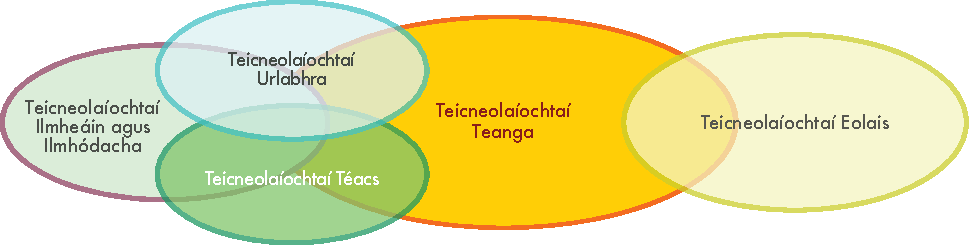
\includegraphics[width=\textwidth]{../_media/irish/language_technologies}
  \caption{Teicneolaíocht Teanga i gComhthéacs}
  \label{fig:ltincontext_de}
  \colorrule{grey3}{\textwidth}{1.5pt}
\end{figure*}

Nuair a dhéanaimid cumarsáid, nascaimid teanga le modhanna eile cumarsáide agus meán faisnéise – mar shampla, tig le comharthaí agus gothaí gnúise bheith mar chuid de labhairt. Nascann téacs digiteach le pictiúir agus fuaimeanna. Tig le teanga i bhfoirm labhartha agus scríofa bheith i scannáin. I bhfocail eile, forluíonn teicneolaíochtaí labhartha agus téacs agus déanann siad idirghníomhú le teicneolaíochtaí eile a éascaíonn próiseáil cumarsáide ilmhódaí agus cáipéisí ilmheáin. 

Sna codanna seo a leanas, pléifimid na príomhréimsí feidhme de theicneolaíocht teanga, i.e. seiceáil teanga, cuardach gréasáin, teicneolaíocht labhartha agus uathaistriú. Áirítear anseo feidhmchláir agus bunteicneolaíochtaí cosúil le

\begin{itemize}
\item ceartú litrithe
\item tacaíocht údaraithe
\item foghlaim teanga ríomhchuidithe
\item aisghabháil faisnéise
\item baint faisnéise
\item achoimriú téacs
\item freagairt ceiste
\item aithint labhartha 
\item sintéis labhartha
\end{itemize}

Is réimse bhunaithe thaighde atá i dteicneolaíocht teanga agus sraith fhairsing litríochta ar fáil ina thaobh. Moltar don léitheoir a bhfuil suim aige ann na tagairtí seo a léamh: \cite{carstensen-etal1} \cite{jurafsky-martin01} \cite{manning-schuetze1} \cite{lt-world1} \cite{lt-survey1}. %NEEDS TO BE TRANSLATED

Sula bpléifimid na réimsí feidhme thuas, déanfaimid cur síos gairid ar ailtireacht an ghnáthchórais TT.

\subsection{Ailtireachtaí Feidhmchláir}

Is iondúil go mbíonn roinnt comhábhar i bhfeidhmchláir bogearraí do phróiseáil teanga a láimhseálann gnéithe éagsúla den teanga. Léiríonn an fíor~\ref{fig:textprocessingarch_de} ailtireacht an-simplithe ar féidir a fháil i ngnáthchóras próiseála téacs (agus ní hionann córas urlabhra agus córas téacs). Láimhseálann an chéad trí mhodúl struchtúr agus brí an ionchuir téacs:

\begin{figure*}[hb]
  \colorrule{grey3}{\textwidth}{1.5pt}
  \center
  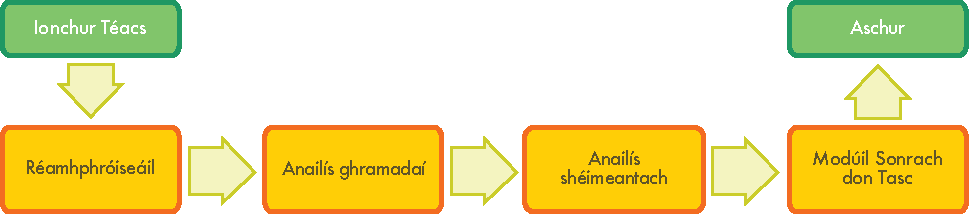
\includegraphics[width=\textwidth]{../_media/irish/text_processing_app_architecture}
  \caption{Ailtireacht Tipiciúil ar Fheidhmchlár Próiseála Téacs}
  \label{fig:textprocessingarch_de}
  \colorrule{grey3}{\textwidth}{1.5pt}
\end{figure*}

\begin{enumerate}
\item Réamhphróiseáil: glantar na sonraí, déantar anailís ar fhormáidiú nó baintear é, braitear an teanga ionchuir, ionadaítear giorrúcháin ``le'd thoil'' in ionad ``le do thoil'', agus mar sin de.
\item Anailís ghramadaí: aimsítear an briathar, a chuspóirí, mionathraitheoirí agus codanna eile den chaint mar aon le struchtúr na habairte a bhrath.
\item Anailís shéimeantach: déantar imdhealú débhríochta (i.e., ríomhtar brí chuí focal i gcomhthéacs ar leith); réitítear iarthagra (i.e., cé na forainmneacha a thagraíonn do na hainmfhocail san abairt) agus ionadaítear teilgean cainte; agus léirítear brí na habairte ar bhealach ar féidir leis an inneall é a léamh.
\end{enumerate}

Tar éis anailís a dhéanamh ar an téacs, tig le modúil tascshonracha feidhmeanna eile a dhéanamh, cosúil le huathachoimriú agus cuardaigh bhunachar sonraí. Is cur síos simplithe agus idéalaithe é seo ar an ailtireacht feidhme agus léiríonn sé castacht na bhfeidhmchlár TT.  

Go ginearálta d’fhéadfaimis ailtireacht fheidhmchláir a rangú ina trí chuid; dóibh siúd atá bunaithe go mórmhór ar rialacha, dóibh siúd atá bunaithe go mórmhór ar staitisticí (dóchúlacht), agus dóibh siúd a chomhshnaidhmeann an dá mhodh. Gintear  samhlacha teanga ó bhailiúcháin ollmhóra teanga (corpas) trí mhodhanna staitisticiúla a úsáid. Go minic, baintear úsáid as corpas ina bhfuil léiriú teangeolaíochta ann, nó corpas lom i dteannta le hacmhainní teangeolaíochta eile ar nós foclóirí nó líonraí séimeantaice. Braitheann caighdeán na samhla staitisticiúla ar chaighdeán na mbunsonraí a úsáidtear mar ionchur. Dá bhrí sin tá acmhainní teangeolaíochta d’ardchaighdeán riachtanach mar chuid de chóras TT, cé gur obair dlúthshaothair é iad a chruthú.

\begin{figure*}[htb]
  \colorrule{grey3}{\textwidth}{1.5pt}
  \center
  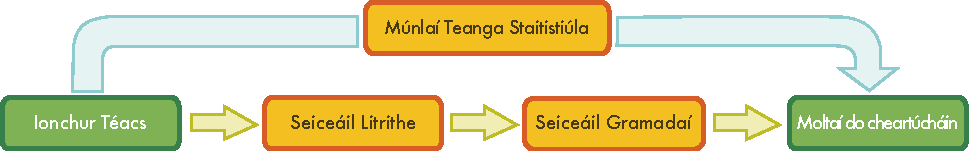
\includegraphics[width=\textwidth]{../_media/irish/language_checking}
  \caption{Seiceáil Teanga (ar bharr: riailbhunaithe; in íochtar: staitistiúil)}
  \label{fig:langcheckingaarch_de}
  \colorrule{grey3}{\textwidth}{1.5pt}
\end{figure*}

Go hiondúil bíonn acmhainní teanga-dhírithe ar nós foclóirí, stórchistí, eolas séimeantach, fóneolaíocht, moirfeolaíocht, agus rialacha gramadaí ag teastáil ó fheidhmchláir TT, chomh maith le corpais (idir téacs agus urlabhra) le léiriú teangeolaíochta ann. Go hidéalach ba cheart go mbeadh an ríomhchláir neamhspleách ar theanga ar leith agus go mbeadh sé in ann oibriú le teanga ar a bith a bhfuil na hacmhainní teanga ábharach ar fáil. Chun leas a bhaint as na feidhmchláir is nua-aimsire sna croíréimsí ar nós uathaistriú, foghlaim teanga ríomhchuidithe, comhéadan  labhartha etc. tá sé fíorthábhachtach go mbeidh na hacmhainní teanga thuasluaite ar fáil. Chomh maith le corpais agus acmhainní teanga, is gá uirlisí teanga ar nós anailíseoir moirfeolaíochta, clibeálaí ranna cainte, parsálaí comhréire, sintéiseoir labhartha agus aithint cainte a bheith ar fáil. Braitheann forbairt na n-uirlisí thuasluaite ar an taighde teangeolaíochta is nua don teanga a bheith ar fáil, ionas go mbeadh na samhlacha riachtanacha  teangeolaíochta  ar fáil.

Tar éis na croíréimsí feidhmchláir a thabhairt isteach do theicneolaíocht teanga, tabharfaimid forbhreathnú gairid ar sheasamh na taighde TT agus an t-oideachas inniu, agus críochnóimid le forbhreathnú ar chláir taighde atá imithe agus atá ann faoi láthair. Ansin cuirfimid meastachán saineolach ar fáil do chroíuirlisí agus acmhainní TT i dtéarmaí na ndiminsean éagsúil cosúil le hinfhaighteacht, aibíocht agus caighdeán. Déantar achoimre ar staid ghinearálta an TT don Ghaeilge i dtábla~\ref{fig:lrlttable_de}.



\subsection{Croíréimsí Feidhme} 

Sa chuid seo, dírimid ar na huirlisí agus acmhainní TT is tábhachtaí, agus tugaimid forbhreathnú ar ghníomhaíochtaí TT in Éirinn. Is féidir uirlisí agus acmhainní a bhfuil líne fúthu sa téacs a aimsiú chomh maith sa tábla ag deireadh na caibidle seo. 

\subsubsection{Seiceáil Teanga}



Tá a fhios ag gach duine a d’úsáid próiseálaí focal cosúil le Microsoft Word go bhfuil seiceálaí litrithe ann a léiríonn botúin litrithe agus a mholann ceartaithe. Chuir na chéad chláir um cheartú litrithe liosta focal aisbhainte i gcomparáid le foclóir focal atá litrithe i gceart. Inniu, tá na cláir seo i bhfad níos sofaisticiúla. Ag baint úsáide as algartaim theangaspleácha d’anailís téacs, braitheann siad earráide a bhaineann le moirfeolaíocht (e.g. foirmiú iolra) mar aon le hearráidí a bhaineann le comhréir, cosúil le briathar in easnamh nó coimhlint le comhaontú briathair-ainmní (e.g. she *write a letter). 

Tá uirlisí seiceála litrithe ar fail don Ghaeilge i sraitheanna oifige cosúil le Microsoft Office agus Open-Office. Ní dhearnadh, áfach, nuashonrú ar sheiceálaí litrithe Microsoft le blianta fada. Níl ach seiceálaí litrithe amháin (GaelSpell http://borel.slu.edu/ispell/) a ndéantar nuashonrú seasta air, d’fhoinse oscailte agus ar fáil do Word/Ooo/Firefox, etc. Tá uirlisí moirfeolaíochta (d’fhoinse oscailte), clibeálaí ranna cainte, agus páirtpharsálaí an spleáchais (http://www.tcd.ie/slscs/itut/) ann  agus an Líonra Séimeantach na Gaeilge d’fhoinse oscailte (http://borel.slu.edu/lsg/).Chomh maith leis sin tá scata feidhmchlár aonair, Foclóir Beag, WinGléacht, EasyReader agus Focal.ie le haghaidh cuardach foclóra agus gramadaí.

Ní hamháin go seiceálann na huirlisí seo litriú ach seiceálann siad go leor gnéithe de ghramadach na Gaeilge, ach ní féidir iad a chomhtháthú go héasca le táirgí atá ann cheana i gcónaí. Mar shampla, ní dhéanann ach seiceálaí teanga amháin don Ghaeilge \cite{gramadoir} níos mó ná ceartú litrithe, agus ní féidir é a chomhtháthú go héasca faoi láthair le OpenOffice ná Microsoft Word (cé go bhfuil an obair seo ar siúl agus an cháipéis seo á scríobh).  

Ach ní bhfaigheadh formhór na seiceálaithe litrithe aon earráidí sa téacs seo \cite{zar1} a leanas: 

\begin{quote}
  I have a spelling checker,\\
  It came with my PC.\\
  It plane lee marks four my revue\\
  Miss steaks aye can knot sea.
\end{quote}

Caithfear anailís a dhéanamh ar an gcomhthéacs comhréire agus shéimeantaigh chun na cineálacha seo earráide a láimhseáil. Caithfidh an cineál seo anailíse tarraingt ar ghramadach theangashonrach atá códaithe go dian ag saineolaithe sna bogearraí nó ar mhúnla teanga staitistiúil. Sa dara chás seo, ríomhann múnla dóchúlacht focail áirithe de réir mar a thagann sé chun cinn in áit ar leith. Is féidir múnla teanga staitistiúil a chruthú go huathoibríoch trí líon mór sonraí teanga (cruinn) a úsáid (ar a dtugtar corpas téacs). Forbraíodh an dá chur chuige seo timpeall ar shonraí ón mBéarla. Faoi láthair, ní féidir le ceachtar cur chuige aistriú go héasca go Gaeilge mar níl mórán acmhainní teanga ar fáil cosúil le corpais téacs chun múnla staitistiúil a chur le chéile agus níl dóthain taighde déanta ar an ionchódú de láimh i ngramadach. Ach tá taighde ar siúil i láthair na huaire ar pharsáil na Gaeilge (\cite{lynn2012}; \cite{elaine2010}).

Níl seiceáil teanga teoranta do phróiseálaithe focail; úsáidtear chomh maith í i ``gcórais tacaíochta údaraithe'', i.e. timpeallachtaí bogearraí ina scríobhtar lámhleabhair agus cáipéisíocht eile chuig caighdeáin speisialta do tháirgí coimpléascacha TF, cúraim shláinte, innealtóireachta agus eile. Tá imní ar chuideachtaí go ndéanfaidh custaiméirí gearáin faoi úsáid mhíchuí agus éilimh dhamáiste mar gheall ar threoracha nár thuig siad i gceart, tá siad ag díriú níos mó ar chaighdeán na cáipéisíochta teicniúla agus ag díriú ar an margadh idirnáisiúnta (trí aistriúchán nó logánú) ag an am céanna. De bharr dul chun cinn i bpróiseáil teanga nádúrtha, forbraíodh bogearraí tacaíochta údaraithe, a chuidíonn le scríbhneoir na cáipéisíochta teicniúla foclóir agus struchtúir abairte a úsáid atá comhsheasmhach le rialacha tionscail agus srianta téarmeolaíochta (corparáideach).

\boxtext{Níl úsáid na seiceála teanga teoranta do phróiseálaithe focail; baineann sé chomh maith le córais tacaíochta údaraithe.} %NEEDS TO BE TRANSLATED

Seachas seiceálaithe litrithe/gramadaí agus tacaíocht údaraithe, tá seiceáil teanga tábhachtach chomh maith i réimse na foghlama teanga ríomhchuidithe. D’fhéadfadh foghlaimeoirí na teanga an-tairbhe a bhaint as fheidhmchláir sa réimse seo. Ach, go dtí seo níl mórán d’fhorbairt déanta sa réimse foghlaim teanga ríomhchuidithe don Ghaeilge. Agus ceartaíonn feidhmchláir seiceála teanga ceisteanna innill chuardaigh go huathoibríoch chomh maith, mar a aimsítear i moltaí \textit{Did you mean~\dots} de chuid Google.

\subsubsection{Cuardach Gréasáin}

\begin{figure*}[htb]
  \colorrule{grey3}{\textwidth}{1.5pt}
  \center
  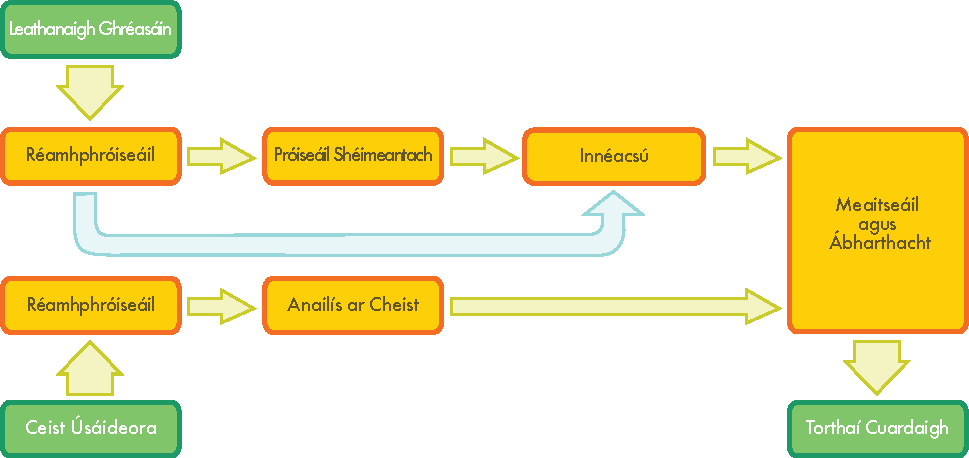
\includegraphics[width=\textwidth]{../_media/irish/web_search_architecture}
  \caption{Ailtireacht do Chuardach Gréasáin}
  \label{fig:websearcharch_de}
  \colorrule{grey3}{\textwidth}{1.5pt}
\end{figure*}


Is é cuardach gréasáin, inlín nó leabharlainne digiteach an feidhmchláir teicneolaíochta teanga is mó a úsáidtear ach is tearcfhorbartha ar domhan. Láimhseálann inneall cuardaigh Google, a thosaigh i 1998, timpeall 80\% de gach cuardach agus os cionn 90\% den uile chuardach ó úsáideoirí idirlín in Éirinn \cite{googlemarketshare}.  ``Gúgláil/googláil'' is ea an briathar oifigiúil i gcomhair ``to google'', a cheadaigh an Coiste Téarmaíochta le déanaí \cite{kilgarriff2010}.  Níor athraíodh comhéadan cuardaigh agus leathanach torthaí Google go suntasach ón gcéad leagan. Ach sa leagan reatha, cuireann Google ceartú litrithe ar fáil d’fhocail nár litríodh i gceart (ach ní don Ghaeilge) agus tá bunchumais chuardaigh shéimeantacha ionchorpraithe anois ar féidir leo cruinneas cuardaigh a fheabhsú trí anailís a dhéanamh ar théarmaí i gcomhthéacs an chuardaigh \cite{googlesemsearch}. Léiríonn scéal ratha Google gur féidir leis an líon mór sonraí atá ar fáil agus teicníochtaí innéacsaithe éifeachtúla torthaí sásúla a sheachadadh do chur chuige staitistiúil. 


D’iarratais faisnéise níos sofaisticiúla , is gá eolas teangeolaíochta níos doimhne a chomhtháthú do \textbf{léirmhíniú téacs}. Léirigh trialacha ag úsáid \textbf{acmhainní foclóireachta} cosúil le teasárais nó acmhainní teanga ointeolaíocha (e.g. WordNet don Bhéarla nó Líonra Séimeantach na Gaeilge don Ghaeilge) feabhsúcháin ar leathanaigh a aimsiú ag úsáid chomhchiallaigh na dtéarmaí cuardaigh bunaigh, cosúil le \textit{fuinnimh adamach} [atomic energy], \textit{cumhacht núicléach} [nuclear energy], nó téarmaí eile a bhfuil baint éigin acu leis.

Beidh ar an gcéad ghlúin eile d’innill chuardaigh teicneolaíocht teanga níos sofaisticiúla a chur san áireamh go háirithe d’fhonn déileáil le cuardaigh ina bhfuil ceist nó cineál abairte eile seachas liosta eochairfhocal. Don cheist, \textit{Tabhair liosta dom do na cuideachtaí ar fad ar ghlac cuideachtaí eile ceannas orthu le cúig bliana anuas} caithfidh an córas TT anailís a dhéanamh ar an abairt ó thaobh comhréire agus séimeantaigh mar aon le hinnéacs a chur ar fáil chun cáipéisí cuí a aimsiú go tapa. Teastóidh parsáil chomhréire do fhreagra sásúil chun anailís a dhéanamh ar struchtúr gramadaí na habairte agus cinneadh a dhéanamh go bhfuil an t-úsáideoir ag iarraidh cuideachtaí a glacadh, ní cuideachtaí a ghlac cuideachtaí eile. Don fhrása \textit{le cúig bliana anuas}, caithfidh an córas cinneadh a dhéanamh maidir leis na blianta ábhartha. Agus, caithfear an cheist a mheaitseáil le méid ollmhór sonraí neamhstruchtúrtha chun píosa nó píosaí eolais ábhartha a theastaíonn ón úsáideoir a fháil. Tugtar ``aisghabháil faisnéise'' air seo, agus baineann sé le cáipéisí ábhartha a chuardach agus a rangú. Chun liosta cuideachtaí a chruthú, caithfidh an córas sraith focal ar leith sa cháipéis a aithint mar ainm cuideachta, próiseas ar a dtugtar ``aithint ainm aonáin''.

\boxtext{Beidh ar an gcéad ghlúin eile d’innill chuardaigh teicneolaíocht teanga níos sofaisticiúla a chur san áireamh.}

Dúshlán níos déine is ea ceist a mheaitseáil i dteanga amháin le cáipéisí i dteanga eile. Baineann aisghabháil faisnéise trasteangaí  le ceist a uathaistriú sna teangacha foinse féideartha ar fad agus ansin na torthaí ar fad a aistriú ar ais go dtí an sprioctheanga. 

Anois agus sonraí á n-aimsiú i bhformáidí neamhthéacsúla, is gá go mbeadh seirbhísí chun aisghabháil faisnéise ilmheáin a sholáthar trí íomhánna, comhaid fuaime agus sonraí físe a chuardach. I gcás comhad fuaime agus físe, caithfidh modúl aitheantais labhartha an t-ábhar labhartha a thiontú ina théacs (nó chuig léirmhíniú foghraíochta) ar féidir é a mheaitseáil in aghaidh ceist úsáideora.

 In Éirinn, cuireann líon beag soláthraithe cosúil le Maithú Teoranta agus grúpaí acadúla éagsúla teicneolaíochta teanga comhábhair ar fáil d’anailís foclóireachta agus tascanna cosúla a d’fhéadfaí a úsáid i gcuardach gréasáin. Tá inneall cuardaigh don Ghaeilge, Aimsigh (http://aimsigh.com), a dearadh don teanga (cuardaigh fréamhaithe etc.) ar fáil ó timpeall 2005--2006. Ach, ar bhotúin an tsaoil, níor baineadh an oiread úsáide as is a bhí tuillte aige, agus úsáideann neart daoine comhéadan Gaeilge Google atá logánaithe ach nach bhfuil optamaithe ná oiriúnaithe le hoibriú sa teanga.
  
\subsubsection{Idirghníomhaíocht Labhartha}

Úsáidtear teicneolaíocht idirghníomhaíochta labhartha chun comhéadain a chruthú a chumasaíonn úsáideoirí le hidirghníomhú i dteanga labhartha in áit amharc grafach, méarchlár agus luchóg. Inniu, is gnách go n-úsáidtear na comhéadain úsáideora chainte (VUI) seo do sheirbhísí teileafóin cuid nó iomlán uathoibríoch a chuireann cuideachtaí ar fáil do chustaiméirí, fostaithe nó comhpháirtithe. Áirítear le fearainn ghnó a bhíonn ag brath go hiomlán ar VUIanna baincéireacht, slabhra soláthair, iompar poiblí agus teileachumarsáid. Áirítear le húsáidí eile de theicneolaíocht chainte comhéadain le córais treoshuímh cairr agus úsáid na teanga labhartha mar rogha mhalartach le comhéadain ghrafacha nó scáileán tadhaill ar ghutháin chliste.

\boxtext{Úsáidtear teicneolaíocht idirghníomhaíochta labhartha mar bhunús le comhéadain a chruthú a cheadaíonn úsáideoirí le hidirghníomhú le teanga labhartha in áit amharc grafach, méarchlár agus luchóg.}

\begin{figure*}[htb]
  \colorrule{grey3}{\textwidth}{1.5pt}
  \center 
  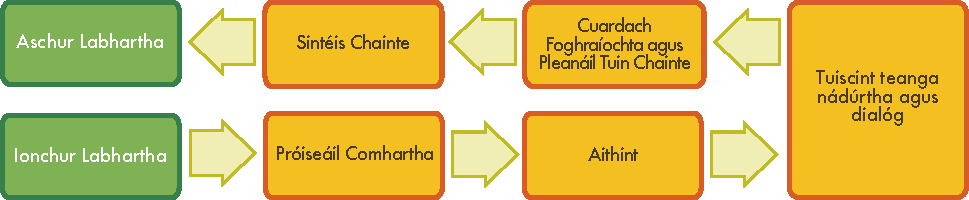
\includegraphics[width=\textwidth]{../_media/irish/simple_speech-based_dialogue_architecture}
  \caption{Córas Dialóige Labhairtbhunaithe}
  \label{fig:dialoguearch_de}
  \colorrule{grey3}{\textwidth}{1.5pt}
\end{figure*}

Tá ceithre theicneolaíocht i dteicneolaíocht labhartha:

\begin{enumerate}
\item \textbf {Aithint cainte} uathoibríoch (ASR) a chinneann cé na focail a deirtear i sraith ar leith fuaimeanna an úsáideora.
\item Déanann tuiscint teanga nádúrtha anailís ar struchtúr comhréir labhartha an úsáideora agus míníonn sí í de réir an chórais atá i gceist.
\item Cinneann bainistíocht dialóige cén gníomh le déanamh de réir ionchur an úsáideora agus fheidhmíocht an chórais.    
\item Aistríonn \textbf{sintéis chainte} (téacs go caint nó TTS) freagra an chórais ina fhuaimeanna don úsáideoir.
\end{enumerate}

Ar cheann de na mórdhúshláin a bhaineann le córais ASR na focail a deir úsáideoirí a aithint go beacht. Is é is ciall leis seo an réimse rudaí a deir an t-úsáideoir a shrianú chuig sraith theoranta eochairfhocal, nó múnlaí teanga a chruthú de láimh a chlúdaíonn réimse leathan teanga nádúrtha. Trí fheidhm a bhaint as teicníochtaí ríomhfhoghlama, is féidir múnlaí teanga a chothú ó chorpais chainte, i.e. bailiúcháin mhóra de chomhaid chainte fuaime agus tras-scríbhinní téacs. Nuair a chuirtear srian ar chaint, is éigean do dhaoine an comhéadan cainte úsáideora a úsáid ar bhealach docht agus déantar damáiste do ghlacadh úsáideora; ach ardófar costais go suntasach de bharr cruthú, tiúnáil agus cothabháil múnla teanga saibhre. Is iondúil go mbíonn VUIanna a úsáideann múnlaí teanga agus a cheadaíonn don úsáideoir a bhfuil i gceist acu a chur in iúl ar bhealach níos solúbtha – a thosaíonn le fáiltiú \textit{Conas is féidir liom cabhair leat?} – uathoibríoch agus glacann úsáideoirí níos fearr leo. 

Is iondúil go n-úsáideann cuideachta cainteoirí gairmiúla chun caint a réamhthaifeadadh chun aschur an chomhéadain úsáideora cainte a chruthú. Do chaint statach nach mbraitheann an fhoclaíocht ar chomhthéacsanna áirithe úsáidte nó sonraí úsáideora pearsanta, tig leis seo taithí níos saibhre a thabhairt don úsáideoir. Ach d’fhéadfadh ábhar níos dinimiciúla bheith beagán mínádúrtha mar gheall gur cuireadh comhaid fuaime randamacha le chéile. Tá córais TTS an lae inniu ag feabhsú (cé gur féidir barrfeabhas a chur orthu) maidir le caint dhinimiciúil nádúrtha a tháirgeadh. 

Rinneadh caighdeánú suntasach ar chomhéadain i margadh na teicneolaíochta labhartha le linn an chéid a caitheadh i dtéarmaí a gcomhábhair theicneolaíochta éagsúla. Bhí comhdhlúthú margaidh láidir in aithint cainte agus sintéis chainte chomh maith. Bhí cúigear imreoirí domhanda i gceannas ar na margaí naisiúnta G20 (tíortha athléimneacha ina bhfuil daonraí arda), le Nuance (S.A.M.) agus Loquendo (an Iodáil) ina n-imreoirí ceannasacha san Eoraip.  In 2011, d’fhógair Nuance gabháil Loquendo, a léiríonn céim eile i gcomhdhlúthú margaidh.

\subsubsection*{Sintéis agus Aithint Labhartha}
Braitheann córais dialóige labhartha go mór ar an teicneolaíocht bhunúsach ar a bhfuil an tsintéis agus aithint labhartha bunaithe. Agus braitheann an tsintéis agus aithint urlabhra ar réimse leathan uirlisí agus acmhainní, nach mbíonn mar chuid de chóras próiseála téacs de ghnáth. Chun gléas sintéise a chur le chéile, mar shampla, caithfidh corpas labhartha a bheith ar fáil, ar a bhfuil trascríobh agus trascanú déanta. Tá gá fosta le foclóirí fuaimnithe, rialacha a aistríonn ón litriú go fuaim, samhail d’fhuaimeanna na teanga, agus samhail den tuinníocht agus den rithim chainte. Mar sin, chun teicneolaíocht na hurlabhra a bhunú do theanga úr, caithfidh go leor anailíse chainníochtúil a bheith déanta roimh réidh ar an teanga labhartha.

Tá a lán taighde ar shintéis na Gaeilge ar siúl (tionscadal ABAIR) san Ionad do Theicneolaíocht Urlabhra agus Teangeolaíochta na Ghaeilge, (ITUT) i gColáiste na Tríonóide (\cite{pittsburgh}). Ós rud é nach raibh an chuid is mó de na hacmhainní riachtanacha ar fáil don Ghaeilge, tá formhór na taighde seo dírithe ar sholáthar na n-acmhainní. Go minic is féidir acmhainní a bhunú go tapaigh do theanga úr ag baint úsáide as modhanna meaisínfhoghlama. Ach leis na deacrachtaí faoi leith a bhaineann leis an Ghaeilge (féach Mír~\ref{AboutIrish_ga}), níor éirigh go ró-mhaith leis na modhanna seo, agus b’éigean córáis lámhscríofa a chruthú. Mar a mhínítear i Mír~\ref{IrishInfso_ga}, caithfidh an teicneolaíocht a bheith in oiriúint don teanga agus don chomhthéacs ina labhraítear í. I gcás na Gaeilge, ba léir ón tús go mbeadh gá le háis a dhéanfadh freastal ar na canúintí éagsúla. Mar gheall air sin, nuair is féidir, tá forbairt á déanamh ar acmhainní mar chodanna ollchanúnacha (a bhaineann le tréithe atá i gcoiteann ag na canúintí) agus codanna chanúnacha (tréithe nach mbaineann ach le canúint amháin). Fágann seo gur féidir athúsáid a bhaint as modúil, agus gur féidir acmhainní a chur ar fáil ar bhealach níos fusa do chanúint úr.

Cuireadh córas sintéise a aistríonn téacs go hurlabhra, an córas ABAIR, ar fáil ar an idirlíon ag www.abair.ie do Ghaeilge Dhún na nGall. Cuirfear glór eile, le canúint Chonamara ar fáil gan mhoill ar an suíomh céanna, agus tá taighde ar siúl faoi láthair ar chanúint Chiarraí, rud atá de dhíth chun freastal ar chainteoirí ón deisceart.

Cé nár déanadh poiblíocht faoi leith dó, agus cé gur ar Ghaeilge an Tuaiscirt amháin atá www.abair.ie ag freastal go dtí seo, tá sé ag dul i bhfeidhm cheana féin ar phobal na Gaeilge in Éirinn agus thar lear. Tugadh cuairt ar an suíomh 40,000 uair i 2011, agus b’as an coimhthíoch breis is leath na gcuairteoirí. Tá sé in úsáid níos mó agus níos mó sna scoileanna, go hairithe i dTuaisceart na hÉireann, mar a bhfuil an chanúint ag fóirstean. Tá múinteoirí, tuistí agus foghlaimeoirí á úsáid. Tá dhá fhadhb le sárú ag an fhoghlaimeoir, lena gcuidíonn sé gur féidir leis éisteacht le téacs á léamh amach. Ar an chéad dul síos, is minic nach mbíonn a fhios ag an fhoghlaimeoir an dóigh le focail scríofa a rá, mar go bhfuil an litriú an-chasta agus go bhfuil fuaimeanna na Gaeilge iontach difriúil ón Bhéarla. Ar an dara dul síos, níl teacht go héasca ag formhór na bhfoghlaimeoirí, in Éirinn nó thar lear, ar chainteoirí dúchais.

Ag freagairt don tsuim atá lucht oideachais na Gaeilge ag cur sa chóras, tá foireann ABAIR ag déanamh forbartha ar áis a chuideoidh le foghlaimeoirí scileanna liteartha agus blas cainte a chothú. Lena chois sin, i gcomhoibriú le grúpaí taighde eile i gColáiste na Tríonóide (\cite {slate2011}), tá cluichí teanga idirghníomhacha á bhforbairt agus ábhair theagaisc atá suite sa saol fíorúla. Tá glórtha sintéise ABAIR mar bhunús acu seo. Tá obair ríthábhachtach a bhfuil gá léi go práinneach ar siúl fosta ag foireann ABAIR chun freastal ar dhaoine atá faoi míchumas radhairc. Is trí mheán na sintéise amháin gur féidir leo seo teacht ar eolas ar an idirlíon agus ar ábhair leictreonacha eile, rud atá riachtanach i bhfoghlaim na Gaeilge, don oideachas trí mheán na Gaeilge. Tá sé riachtanach fosta le cur ar a gcumas páirt iomlán a ghlacadh i mórán imeachtaí a bhaineann le pobal na Gaeilge.

Cé go bhfuil go leor bainte amach go dtí seo, tá méid mór oibre le déanamh go fóill chun an dúshraith seo a dhaingniú, agus chun na corpais, na glórthaí sintéise agus na hacmhainní a bhaineann leo a fhorbairt go dtí an leibhéal ag a bhfuil a macasamhail sna mórtheangacha.     

Sa réimse a bhaineann le haithint labhartha, níl aon fhorbairt déanta fós. Mar sin féin, tá méid áirithe den dúshraith á forbairt, sa mhéid is gur ionann a lán de na hacmhainní don aithint labhartha agus iad siúd atá á bhforbairt don tsintéis. Ach beidh gá le corpais ollmhóra labhartha le trascríobh iomlán foghraíochta, chun an réimse seo a thabhairt ar aghaidh. Mar sin, tá bealach fada le dul sula mbíonn muid in ann córais dialóige labhartha a chur ar fáil don Ghaeilge. Cé go bhfuil cuid de na píosaí á gcur ar fáil de réir a chéile, tá cuid eile, cosúil le aithint labhartha, a bhfuil forbairt iomlán le déanamh orthu go fóill.


Faoi láthair, tá teicneolaíocht na hurlabhra don Ghaeilge PC-bhunaithe, don chuid is mó, cé go bhfuil ceann nó dhó ar fáil. Ach sa todhchaí, tarlóidh athruithe suntasacha de bharr scaipeadh guthán cliste mar léibheann nua chun caidreamh custaiméara a bhainistiú anuas ar theileafóin sheasta, ar an Idirlíon agus ar an ríomhphost. Beidh tionchar aige seo ar an gcaoi a n-úsáidfear teicneolaíocht idirchaidrimh chainte. Don fhadtréimhse, beidh níos lú VUIanna teileafónbhunaithe agus beidh ról i bhfad níos lárnaí ag an teanga labhartha amhail ionchur soláimhsithe do ghutháin chliste. Tiomáinfidh feabhsúcháin chéimnithe é seo go príomha i gcruinneas aithint cainte neamhspleách ar chainteoir trí sheirbhísí deachtúcháin a chuirtear ar fáil cheana mar sheirbhísí lárnaithe d’úsáideoirí guthán cliste.


\subsubsection{Uathaistriú}

Téann an smaoineamh maidir le ríomhairí digiteacha a úsáid le teangacha nádúrtha a aistriú siar go dtí 1946 agus tháinig maoiniú suntasach ina dhiaidh sin do thaighde sna 1950idí agus arís sna 1980idí. Ach fós féin, ní féidir le \textbf{huathaistriú} (``machine translation,'' MT) an rud a rabhthas ag súil uaidh a chomhlíonadh, is é sin uathaistriú cuimsitheach. 

\boxtext{Ag a leibhéal bunúsach, ionadaíonn Uathaistriú focail i dteanga nádúrtha amháin le focail i dteanga eile.}

Is é an cur chuige is bunúsaí le huathaistriúchán focail i dtéacs i dteanga nádúrtha amháin a ionadú go huathoibríoch le focail i dteanga eile. Tig leis seo bheith an-úsáideach i bhfearainn ainmní ina bhfuil teanga foirmleach an-srianta cosúil le tuairiscí aimsire. Ach, chun dea-aistriúchán a chur ar fáil do théacsanna nach bhfuil caighdeánaithe, caithfear aonaid téacs níos mó (frásaí, abairtí, nó pasáistí iomlána) a mheaitseáil lena macasamhail sa sprioctheanga. Is é an mórdheacracht go bhfuil teanga dhaonna débhríoch. Cruthaíonn débhríochas dúshláin ar il-leibhéil, cosúil le débhríochas focail ar leibhéal foclóireachta (is branda cairr nó ainmhí atá in \textit{jaguar}).

Bealach amháin le córas MT a thógáil is ea rialacha teangeolaíocha a úsáid. D’aistriúcháin idir teangacha le gaol gar eatarthu, d’fhéadfaí aistriúchán ionadaithe dhírigh a úsáid i gcásanna cosúil leis an sampla thuas. Ach, go minic déanann córais riailbhunaithe (nó eolasbhunaithe teangeolaíochta) anailís ar an téacs ionchuir agus cruthaíonn siad léiriú siombalach idirmheánach ónar féidir an téacs a chruthú sa sprioctheanga. Braitheann rath na modhanna seo ar infhaighteacht foclóirí fairsinge le faisnéis mhoirfeolaíochta, chomhréire agus shéimeantach, agus sraitheanna níos mó de rialacha gramadaí a dhear teangeolaithe oilte go cúramach. Is próiseas an-fhada agus dá bhrí sin, costasach atá anseo.

\begin{figure*}[htb]
  \colorrule{grey3}{\textwidth}{1.5pt}
  \center
  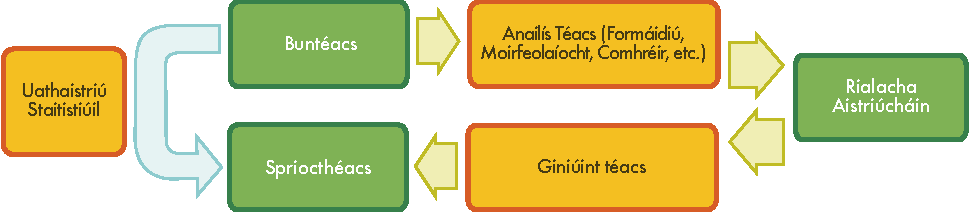
\includegraphics[width=\textwidth]{../_media/irish/machine_translation}
  \caption{Uathaistriú (ar chlé: staitistiúil, ar dheis: riailbhunaithe)}
  \label{fig:mtarch_de}
  \colorrule{grey3}{\textwidth}{1.5pt}
\end{figure*}

Go déanach sna 1980idí nuair a d’fheabhsaigh cumhacht ríomhaireachta agus a laghdaigh sé i gcostas, ach bhí suim níos mó i múnlaí staitistiúla d’uathaistriú. Eascraíonn múnlaí staitistiúla ó anailís a dhéanamh ar chorpais téacs dhátheangacha, cosúil le \textbf{corpais chomhthreomhara} Europarl, ina bhfuil imeachtaí Pharlaimint na hEorpa in 11 theanga Eorpacha. Má chuirtear dóthain sonraí ann, oibríonn MT staitistiúil sách maith chun míniú measta a bhaint as téacs i dteanga iasachta trí leaganacha comhthreomhara a phróiseáil agus pátrúin focail sochreidte a aimsiú. Ach, neamhchosúil le córais eolasbhunaithe, cruthaíonn MT staitistiúil (nó sonraíbhunaithe) aschur neamhghramadaí go minic. Tá buntáistí ag baint le MT sonraíbhunaithe mar nach dteastaíonn an oiread iarracht dhaonna, agus tig leis sonraíochtaí speisialta den teanga a chlúdach (e.g. leaganacha cainte) a dtugtar neamhaird orthu i gcórais eolasbhunaithe. 

Is iondúil go mbíonn na láidreachtaí agus na laigí atá ag uathaistriú eolasbhunaithe agus sonraíbhunaithe comhlántach, agus anois díríonn taighdeoirí ar chur chuige hibride a úsáideann an dá mhodheolaíocht. Úsáideann cur chuige amháin córais eolasbhunaithe agus sonraíbhunaithe mar aon le modúl roghnaithe a dhéanann cinneadh ar an aschur is fearr do gach abairt. Ach, ní bheidh torthaí d'abairtí níos faide ná 12 fhocal foirfe in aon chor. Réiteach níos fearr is ea na codanna is fearr do gach abairt as ilaschuir a cheangal; tig leis seo bheith réasúnta coimpléascach, mar nach mbíonn codanna comhfhreagracha de roghanna malartacha soiléir i gcónaí agus caithfear ailíniú a dhéanamh orthu. 

\boxtext{De bharr easpa sonraí, tá dúshlán ar leith ag baint le hUathaistriú don Ghaeilge.} 

Cé go bhfuil obair cheannródaíoch déanta don Ghaeilge i réimse na gcuimhní aistriúcháin, tá cumas mór fós ann do chaighdeán na gcóras MT a fheabhsú. Baineann na dúshláin le hacmhainní teanga a oiriúnú chuig fearainn ainmní nó réimse úsáideora, agus an teicneolaíocht a chomhtháthú ina shreabhadh oibre ina bhfuil bunachair théarmaí agus cuimhní aistriúcháin cheana. Fadhb eile is ea go bhfuil formhór na gcóras reatha bunaithe ar an mBéarla agus ní thacaíonn mórán acu le Gaeilge. Dá bharr seo bíonn frithchuimilt sa sreabhadh oibre aistriúcháin agus cuireann sé brú ar úsáideoirí MT uirlisí códaithe foclóireachta éagsúla a fhoghlaim do chórais éagsúla. 


Tá roinnt obair tionsclaíocha déanta ar chóras uathaistrithe don Ghaeilge ag Traslan Teoranta, atá ceannaithe ag an chomhlacht Sasanach Applied Language Solutions le déanaí. Feidhmíonn an córas móréilimh Google Translate le Gaeilge go pointe áirithe chomh maith. Ach tá easpa acmhainní teanga (corpais comhthreomhar, agus foclóirí dátheangacha) ina chonstaic ar fhorbairt bhreise a dhéanamh ar chóras uathaistrithe don Ghaeilge.

Cuidíonn feachtais luachála comparáid a dhéanamh idir caighdeán na gcóras MT, an cur chuige éagsúil agus stádas na gcóras do phéirí teanga éagsúla. Léiríonn an tábla~\ref{fig:euromatrix_de} thíos, a réitíodh le linn thionscadal EC Euromatrix+, na feidhmíochtaí bunaithe ar phéirí a baineadh amach do 22 de na 23 teanga oifigiúil Eorpach. (Ní raibh an Ghaeilge san áireamh sa chomparáid de bharr easpa uirlisí bheith ar fáil.) Rangaíodh na torthaí de réir scór BLEU, a léiríonn scóir níos airde d’aistriúcháin níos fearr \cite{bleu1}. Gheobhadh aistritheoir daonna scór timpeall 80 pointe.

Baineadh amach na torthaí is fearr (i nglas agus gorm) i dteangacha a fhaigheann buntáiste as taighde suntasach i gcláir chomhordaithe agus ó na corpais chomhthreomhara a bhí ann (e.g. Béarla, Fraincis, Ollainnis, Spáinnis agus Gearmáinis). Léirítear na teangacha le torthaí níos measa i ndearg. Níl iarrachtaí forbartha ag na teangacha seo nó tá struchtúr an-difriúil acu ó na teangacha eile (e.g. Ungáiris, Máltais agus Fionlainnis).

\begin{figure*}[htbp]
  \centering
  \setlength{\tabcolsep}{0.17em}
  \small
  \begin{tabular}{>{\columncolor{corange1}}cccccccccccccccccccccccc}
    & \multicolumn{22}{>{\columncolor{corange1}}c}{Sprioctheanga -- \textcolor{grey1}{Target language}}\\\addlinespace[{-.009cm}] %NEEDS TO BE TRANSLATED
    \rowcolor{corange1}  & EN & BG & DE & CS & DA & EL & ES & ET & FI & FR & HU & IT & LT & LV & MT & NL & PL & PT & RO & SK & SL & SV\\
    EN & -- & \textcolor{blue}{40.5} & \textcolor{blue}{46.8} & \textcolor{green2}{52.6} & \textcolor{green2}{50.0} & \textcolor{blue}{41.0} & \textcolor{green2}{55.2} & \textcolor{purple}{34.8} & \textcolor{purple}{38.6} & \textcolor{green2}{50.1} & \textcolor{purple}{37.2} & \textcolor{green2}{50.4} & \textcolor{purple}{39.6} & \textcolor{blue}{43.4} & \textcolor{purple}{39.8} & \textcolor{green2}{52.3} & \textcolor{blue}{49.2} & \textcolor{green2}{55.0} & \textcolor{blue}{49.0} & \textcolor{blue}{44.7} & \textcolor{green2}{50.7} & \textcolor{green2}{52.0}\\
    BG & \textcolor{green}{61.3} & -- & \textcolor{purple}{38.7} & \textcolor{purple}{39.4} & \textcolor{purple}{39.6} & \textcolor{purple}{34.5} & \textcolor{blue}{46.9} & \textcolor{red3}{25.5} & \textcolor{red3}{26.7} & \textcolor{blue}{42.4} & \textcolor{red3}{22.0} & \textcolor{blue}{43.5} & \textcolor{red3}{29.3} & \textcolor{red3}{29.1} & \textcolor{red3}{25.9} & \textcolor{blue}{44.9} & \textcolor{purple}{35.1} & \textcolor{blue}{45.9} & \textcolor{purple}{36.8} & \textcolor{purple}{34.1} & \textcolor{purple}{34.1} & \textcolor{purple}{39.9}\\
    DE & \textcolor{green2}{53.6} & \textcolor{red3}{26.3} & -- & \textcolor{purple}{35.4} & \textcolor{blue}{43.1} & \textcolor{purple}{32.8} & \textcolor{blue}{47.1} & \textcolor{red3}{26.7} & \textcolor{red3}{29.5} & \textcolor{purple}{39.4} & \textcolor{red3}{27.6} & \textcolor{blue}{42.7} & \textcolor{red3}{27.6} & \textcolor{purple}{30.3} & \textcolor{red2}{19.8} & \textcolor{green2}{50.2} & \textcolor{purple}{30.2} & \textcolor{blue}{44.1} & \textcolor{purple}{30.7} & \textcolor{red3}{29.4} & \textcolor{purple}{31.4} & \textcolor{blue}{41.2}\\
    CS & \textcolor{green2}{58.4} & \textcolor{purple}{32.0} & \textcolor{blue}{42.6} & -- & \textcolor{blue}{43.6} & \textcolor{purple}{34.6} & \textcolor{blue}{48.9} & \textcolor{purple}{30.7} & \textcolor{purple}{30.5} & \textcolor{blue}{41.6} & \textcolor{red3}{27.4} & \textcolor{blue}{44.3} & \textcolor{purple}{34.5} & \textcolor{purple}{35.8} & \textcolor{red3}{26.3} & \textcolor{blue}{46.5} & \textcolor{purple}{39.2} & \textcolor{blue}{45.7} & \textcolor{purple}{36.5} & \textcolor{blue}{43.6} & \textcolor{blue}{41.3} & \textcolor{blue}{42.9}\\
    DA & \textcolor{green2}{57.6} & \textcolor{red3}{28.7} & \textcolor{blue}{44.1} & \textcolor{purple}{35.7} & -- & \textcolor{purple}{34.3} & \textcolor{blue}{47.5} & \textcolor{red3}{27.8} & \textcolor{purple}{31.6} & \textcolor{blue}{41.3} & \textcolor{red3}{24.2} & \textcolor{blue}{43.8} & \textcolor{red3}{29.7} & \textcolor{purple}{32.9} & \textcolor{red3}{21.1} & \textcolor{blue}{48.5} & \textcolor{purple}{34.3} & \textcolor{blue}{45.4} & \textcolor{purple}{33.9} & \textcolor{purple}{33.0} & \textcolor{purple}{36.2} & \textcolor{blue}{47.2}\\
    EL & \textcolor{green2}{59.5} & \textcolor{purple}{32.4} & \textcolor{blue}{43.1} & \textcolor{purple}{37.7} & \textcolor{blue}{44.5} & -- & \textcolor{green2}{54.0} & \textcolor{red3}{26.5} & \textcolor{red3}{29.0} & \textcolor{blue}{48.3} & \textcolor{red3}{23.7} & \textcolor{blue}{49.6} & \textcolor{red3}{29.0} & \textcolor{purple}{32.6} & \textcolor{red3}{23.8} & \textcolor{blue}{48.9} & \textcolor{purple}{34.2} & \textcolor{green2}{52.5} & \textcolor{purple}{37.2} & \textcolor{purple}{33.1} & \textcolor{purple}{36.3} & \textcolor{blue}{43.3}\\
    ES & \textcolor{green}{60.0} & \textcolor{purple}{31.1} & \textcolor{blue}{42.7} & \textcolor{purple}{37.5} & \textcolor{blue}{44.4} & \textcolor{purple}{39.4} & -- & \textcolor{red3}{25.4} & \textcolor{red3}{28.5} & \textcolor{green2}{51.3} & \textcolor{red3}{24.0} & \textcolor{green2}{51.7} & \textcolor{red3}{26.8} & \textcolor{purple}{30.5} & \textcolor{red3}{24.6} & \textcolor{blue}{48.8} & \textcolor{purple}{33.9} & \textcolor{green2}{57.3} & \textcolor{purple}{38.1} & \textcolor{purple}{31.7} & \textcolor{purple}{33.9} & \textcolor{blue}{43.7}\\
    ET & \textcolor{green2}{52.0} & \textcolor{red3}{24.6} & \textcolor{purple}{37.3} & \textcolor{purple}{35.2} & \textcolor{purple}{37.8} & \textcolor{red3}{28.2} & \textcolor{blue}{40.4} & -- & \textcolor{purple}{37.7} & \textcolor{purple}{33.4} & \textcolor{purple}{30.9} & \textcolor{purple}{37.0} & \textcolor{purple}{35.0} & \textcolor{purple}{36.9} & \textcolor{red3}{20.5} & \textcolor{blue}{41.3} & \textcolor{purple}{32.0} & \textcolor{purple}{37.8} & \textcolor{red3}{28.0} & \textcolor{purple}{30.6} & \textcolor{purple}{32.9} & \textcolor{purple}{37.3}\\
    FI & \textcolor{blue}{49.3} & \textcolor{red3}{23.2} & \textcolor{purple}{36.0} & \textcolor{purple}{32.0} & \textcolor{purple}{37.9} & \textcolor{red3}{27.2} & \textcolor{purple}{39.7} & \textcolor{purple}{34.9} & -- & \textcolor{red3}{29.5} & \textcolor{red3}{27.2} & \textcolor{purple}{36.6} & \textcolor{purple}{30.5} & \textcolor{purple}{32.5} & \textcolor{red2}{19.4} & \textcolor{blue}{40.6} & \textcolor{red3}{28.8} & \textcolor{purple}{37.5} & \textcolor{red3}{26.5} & \textcolor{red3}{27.3} & \textcolor{red3}{28.2} & \textcolor{purple}{37.6}\\
    FR & \textcolor{green}{64.0} & \textcolor{purple}{34.5} & \textcolor{blue}{45.1} & \textcolor{purple}{39.5} & \textcolor{blue}{47.4} & \textcolor{blue}{42.8} & \textcolor{green}{60.9} & \textcolor{red3}{26.7} & \textcolor{purple}{30.0} & -- & \textcolor{red3}{25.5} & \textcolor{green2}{56.1} & \textcolor{red3}{28.3} & \textcolor{purple}{31.9} & \textcolor{red3}{25.3} & \textcolor{green2}{51.6} & \textcolor{purple}{35.7} & \textcolor{green}{61.0} & \textcolor{blue}{43.8} & \textcolor{purple}{33.1} & \textcolor{purple}{35.6} & \textcolor{blue}{45.8}\\
    HU & \textcolor{blue}{48.0} & \textcolor{red3}{24.7} & \textcolor{purple}{34.3} & \textcolor{purple}{30.0} & \textcolor{purple}{33.0} & \textcolor{red3}{25.5} & \textcolor{purple}{34.1} & \textcolor{red3}{29.6} & \textcolor{red3}{29.4} & \textcolor{purple}{30.7} & -- & \textcolor{purple}{33.5} & \textcolor{red3}{29.6} & \textcolor{purple}{31.9} & \textcolor{red2}{18.1} & \textcolor{purple}{36.1} & \textcolor{red3}{29.8} & \textcolor{purple}{34.2} & \textcolor{red3}{25.7} & \textcolor{red3}{25.6} & \textcolor{red3}{28.2} & \textcolor{purple}{30.5}\\
    IT & \textcolor{green}{61.0} & \textcolor{purple}{32.1} & \textcolor{blue}{44.3} & \textcolor{purple}{38.9} & \textcolor{blue}{45.8} & \textcolor{blue}{40.6} & \textcolor{red3}{26.9} & \textcolor{red3}{25.0} & \textcolor{red3}{29.7} & \textcolor{green2}{52.7} & \textcolor{red3}{24.2} & -- & \textcolor{red3}{29.4} & \textcolor{purple}{32.6} & \textcolor{red3}{24.6} & \textcolor{green2}{50.5} & \textcolor{purple}{35.2} & \textcolor{green2}{56.5} & \textcolor{purple}{39.3} & \textcolor{purple}{32.5} & \textcolor{purple}{34.7} & \textcolor{blue}{44.3}\\
    LT & \textcolor{green2}{51.8} & \textcolor{red3}{27.6} & \textcolor{purple}{33.9} & \textcolor{purple}{37.0} & \textcolor{purple}{36.8} & \textcolor{red3}{26.5} & \textcolor{red3}{21.1} & \textcolor{purple}{34.2} & \textcolor{purple}{32.0} & \textcolor{purple}{34.4} & \textcolor{red3}{28.5} & \textcolor{purple}{36.8} & -- & \textcolor{blue}{40.1} & \textcolor{red3}{22.2} & \textcolor{purple}{38.1} & \textcolor{purple}{31.6} & \textcolor{purple}{31.6} & \textcolor{red3}{29.3} & \textcolor{purple}{31.8} & \textcolor{purple}{35.3} & \textcolor{purple}{35.3}\\
    LV & \textcolor{green2}{54.0} & \textcolor{red3}{29.1} & \textcolor{purple}{35.0} & \textcolor{purple}{37.8} & \textcolor{purple}{38.5} & \textcolor{red3}{29.7} & \textcolor{red2}{8.0} & \textcolor{purple}{34.2} & \textcolor{purple}{32.4} & \textcolor{purple}{35.6} & \textcolor{red3}{29.3} & \textcolor{purple}{38.9} & \textcolor{purple}{38.4} & -- & \textcolor{red3}{23.3} & \textcolor{blue}{41.5} & \textcolor{purple}{34.4} & \textcolor{purple}{39.6} & \textcolor{purple}{31.0} & \textcolor{purple}{33.3} & \textcolor{purple}{37.1} & \textcolor{purple}{38.0}\\
    MT & \textcolor{green}{72.1} & \textcolor{purple}{32.2} & \textcolor{purple}{37.2} & \textcolor{purple}{37.9} & \textcolor{purple}{38.9} & \textcolor{purple}{33.7} & \textcolor{blue}{48.7} & \textcolor{red3}{26.9} & \textcolor{red3}{25.8} & \textcolor{blue}{42.4} & \textcolor{red3}{22.4} & \textcolor{blue}{43.7} & \textcolor{purple}{30.2} & \textcolor{purple}{33.2} & -- & \textcolor{blue}{44.0} & \textcolor{purple}{37.1} & \textcolor{blue}{45.9} & \textcolor{purple}{38.9} & \textcolor{purple}{35.8} & \textcolor{blue}{40.0} & \textcolor{blue}{41.6}\\
    NL & \textcolor{green2}{56.9} & \textcolor{red3}{29.3} & \textcolor{blue}{46.9} & \textcolor{purple}{37.0} & \textcolor{blue}{45.4} & \textcolor{purple}{35.3} & \textcolor{blue}{49.7} & \textcolor{red3}{27.5} & \textcolor{red3}{29.8} & \textcolor{blue}{43.4} & \textcolor{red3}{25.3} & \textcolor{blue}{44.5} & \textcolor{red3}{28.6} & \textcolor{purple}{31.7} & \textcolor{red3}{22.0} & -- & \textcolor{purple}{32.0} & \textcolor{blue}{47.7} & \textcolor{purple}{33.0} & \textcolor{purple}{30.1} & \textcolor{purple}{34.6} & \textcolor{blue}{43.6}\\
    PL & \textcolor{green}{60.8} & \textcolor{purple}{31.5} & \textcolor{blue}{40.2} & \textcolor{blue}{44.2} & \textcolor{blue}{42.1} & \textcolor{purple}{34.2} & \textcolor{blue}{46.2} & \textcolor{red3}{29.2} & \textcolor{red3}{29.0} & \textcolor{blue}{40.0} & \textcolor{red3}{24.5} & \textcolor{blue}{43.2} & \textcolor{purple}{33.2} & \textcolor{purple}{35.6} & \textcolor{red3}{27.9} & \textcolor{blue}{44.8} & -- & \textcolor{blue}{44.1} & \textcolor{purple}{38.2} & \textcolor{purple}{38.2} & \textcolor{purple}{39.8} & \textcolor{blue}{42.1}\\
    PT & \textcolor{green}{60.7} & \textcolor{purple}{31.4} & \textcolor{blue}{42.9} & \textcolor{purple}{38.4} & \textcolor{blue}{42.8} & \textcolor{blue}{40.2} & \textcolor{green}{60.7} & \textcolor{red3}{26.4} & \textcolor{red3}{29.2} & \textcolor{green2}{53.2} & \textcolor{red3}{23.8} & \textcolor{green2}{52.8} & \textcolor{red3}{28.0} & \textcolor{purple}{31.5} & \textcolor{red3}{24.8} & \textcolor{blue}{49.3} & \textcolor{purple}{34.5} & -- & \textcolor{purple}{39.4} & \textcolor{purple}{32.1} & \textcolor{purple}{34.4} & \textcolor{blue}{43.9}\\
    RO & \textcolor{green}{60.8} & \textcolor{purple}{33.1} & \textcolor{purple}{38.5} & \textcolor{purple}{37.8} & \textcolor{blue}{40.3} & \textcolor{purple}{35.6} & \textcolor{green2}{50.4} & \textcolor{red3}{24.6} & \textcolor{red3}{26.2} & \textcolor{blue}{46.5} & \textcolor{red3}{25.0} & \textcolor{blue}{44.8} & \textcolor{red3}{28.4} & \textcolor{red3}{29.9} & \textcolor{red3}{28.7} & \textcolor{blue}{43.0} & \textcolor{purple}{35.8} & \textcolor{blue}{48.5} & -- & \textcolor{purple}{31.5} & \textcolor{purple}{35.1} & \textcolor{purple}{39.4}\\
    SK & \textcolor{green}{60.8} & \textcolor{purple}{32.6} & \textcolor{purple}{39.4} & \textcolor{blue}{48.1} & \textcolor{blue}{41.0} & \textcolor{purple}{33.3} & \textcolor{blue}{46.2} & \textcolor{red3}{29.8} & \textcolor{red3}{28.4} & \textcolor{purple}{39.4} & \textcolor{red3}{27.4} & \textcolor{blue}{41.8} & \textcolor{purple}{33.8} & \textcolor{purple}{36.7} & \textcolor{red3}{28.5} & \textcolor{blue}{44.4} & \textcolor{purple}{39.0} & \textcolor{blue}{43.3} & \textcolor{purple}{35.3} & -- & \textcolor{blue}{42.6} & \textcolor{blue}{41.8}\\
    SL & \textcolor{green}{61.0} & \textcolor{purple}{33.1} & \textcolor{purple}{37.9} & \textcolor{blue}{43.5} & \textcolor{blue}{42.6} & \textcolor{purple}{34.0} & \textcolor{blue}{47.0} & \textcolor{purple}{31.1} & \textcolor{red3}{28.8} & \textcolor{purple}{38.2} & \textcolor{red3}{25.7} & \textcolor{blue}{42.3} & \textcolor{purple}{34.6} & \textcolor{purple}{37.3} & \textcolor{purple}{30.0} & \textcolor{blue}{45.9} & \textcolor{purple}{38.2} & \textcolor{blue}{44.1} & \textcolor{purple}{35.8} & \textcolor{purple}{38.9} & -- & \textcolor{blue}{42.7}\\
    SV & \textcolor{green2}{58.5} & \textcolor{red3}{26.9} & \textcolor{blue}{41.0} & \textcolor{purple}{35.6} & \textcolor{blue}{46.6} & \textcolor{purple}{33.3} & \textcolor{blue}{46.6} & \textcolor{red3}{27.4} & \textcolor{purple}{30.9} & \textcolor{purple}{38.9} & \textcolor{red3}{22.7} & \textcolor{blue}{42.0} & \textcolor{red3}{28.2} & \textcolor{purple}{31.0} & \textcolor{red3}{23.7} & \textcolor{blue}{45.6} & \textcolor{purple}{32.2} & \textcolor{blue}{44.2} & \textcolor{purple}{32.7} & \textcolor{purple}{31.3} & \textcolor{purple}{33.5} & --\\
    \end{tabular}
  \caption{Uathaistriú idir 22 Theanga AE -- \textcolor{grey1}{Machine translation between 22 EU-languages \cite{euro1}}} 
  \label{fig:euromatrix_de}
\end{figure*}

\subsection{Réimsí Eile Feidhme}

Baineann réimse fothascanna nach bhfeictear ag leibhéal na hidirghníomhaíochta leis an úsáideoir i gcónaí, le feidhmchláir teicneolaíochta teanga a thógáil, ach cuireann siad feidhmeanna seirbhíse suntasacha “laistigh” den chóras atá i gceist. Bíonn siad ar fad mar chuid de shaincheisteanna taighde atá fásta anois ina bhfodhisciplíní aonair de ríomhtheangeolaíocht agus eolaíocht na hurlabhra. 

\boxtext{Cuireann feidhmchláir teicneolaíochta teanga feidhmeanna seirbhíse suntasacha ar fáil “laistigh” de chórais bhogearraí níos mó.}

Is réimse taighde ghníomhaigh atá i bhfreagairt ceisteanna, mar shampla, lenar tógadh corpais anótáilte (don Bhéarla go príomha) agus lenar tosaíodh comórtais eolaíochta. Téann coincheap freagairte ceisteanna níos faide ná cuardaigh bunaithe ar eochairfhocail (ina bhfreagraíonn an t-inneall cuardaigh trí bhailiúchán cáipéisí a d’fhéadfadh bheith ábhartha a sheachadadh) agus a chumasaíonn úsáideoirí ceist a chur agus go dtugann an córas freagra amháin air. Mar shampla:

\textit{Ceist: Cén aois a bhí Neil Armstrong nuair a sheas sé ar an ngealach?}\\
\textit{Freagra: 38.}

Cé go bhfuil gaol ag freagairt ceisteanna le croíréimse an chuardaigh ghréasáin, is brat-téarma é seo anois ar shaincheisteanna taighde den chineál seo maidir leis na cineálacha éagsúla ceisteanna atá ann, agus an chaoi ar cheart iad a láimhseáil; conas anailís agus comparáid a dhéanamh ar shraith cáipéisí ina bhféadfadh an freagra a bheith (an dtugann siad freagraí coimhlinte?); agus an chaoi ar féidir eolas ar leith (an freagra) a bhaint i gceart as cáipéis gan neamhaird a thabhairt ar an gcomhthéacs. 

Bhain sé seo ina dhiaidh sin le baint faisnéise (IE), réimse a raibh an-tóir air agus a raibh tionchar aige nuair a chuaigh teangeolaíocht ríomhaireachta i dtreo staitistiúil ag tús na 1990idí. Díríonn IE ar phíosaí ar leith faisnéise a aithint i gcineálacha áirithe cáipéisí, cosúil le príomhpháirtithe i ngabhálacha cuideachta a aithint amhail a tuairiscíodh iad i scéalta nuachtáin. Cás coitianta eile a ndearnadh staidéar air is ea tuairiscí ar eachtraí sceimhlitheoireachta. Is í an fhadhb anseo an teacs a léarscáiliú chuig teimpléad a leagann amach déantóir na hoibre, sprioc, am, láthair agus torthaí na heachtra. Tá líonadh teimpléid fearainnshonrach ina shaintréith lárnach de IE, atá ina shampla eile de theicneolaíocht ``laistigh'' atá ina chuid de réimse taighde dea-chríochaithe a chaithfear bheith leabaithe i dtimpeallacht feidhmchláir oiriúnaigh i gcleachtadh.

Is dhá réimse teorann iad achoimriú agus \textbf{giniúint téacs} ar féidir leo feidhmiú mar fheidhmchláir astu féin nó ról tacaíochta bheith acu ``laistigh''. Déantar iarracht le hachoimriú na nithe is ríthábhachtaí as téacs fada a thabhairt i leagan gearr, agus tá sé ar cheann de na gnéithe atá ar fáil in Microsoft Word.  Úsáideann sé cur chuige staitistiúil den chuid is mó chun na focail ``thábhachtacha'' i dtéacs a shainaithint (i.e. focail a fheictear go minic sa téacs atá i gceist ach nach mbíonn chomh minic i ngnáthúsáid teanga) agus cinneadh a dhéanamh maidir leis na habairtí ina bhfuil na focail is ``tábhachtaí''. Ansin, baintear amach na habairtí seo agus cuirtear le chéile iad chun achoimre a chruthú. Is cás tráchtála an-choitianta é seo, níl in achoimriú ach saghas bainte abairtí, agus laghdaítear an téacs chuig foshraith a abairtí. Cur chuige malartach, ar a ndearnadh roinnt taighde, is ea chun branda nua abairtí a ghiniúint nach bhfuil ar fáil sa bhuntéacs. Tá tuiscint níos doimhne ag teastáil ar an téacs dó seo, agus dá bharr seo níl an cur chuige seo chomh láidir. Ar an iomlán, is annamh a úsáidtear ginteoir téacs mar fheidhmchlár as féin ach bíonn sé leabaithe i dtimpeallacht bogearraí níos mó cosúil le córas faisnéise cliniciúil a bhailíonn, a stórálann agus a phróiseálann sonraí othair.  Níl i gcruthú tuairiscí ach ceann de na feidhmeanna d’achoimriú téacs.  

Don Ghaeilge, níl an oiread forbartha déanta ar na teicneolaíochtaí téacs seo is atá do theangacha Eorpacha eile. Díríodh ar fhreagairt ceisteanna, baint faisnéise agus achoimriú i roinnt comórtais oscailte i S.A.M. ó na 1990idí, á n-eagrú go príomha ag eagraíochtaí urraithe ag an rialtas DARPA agus NIST. D’fheabhsaigh na comórtais seo an teicneolaíocht úrscothach, ach dhírigh siad den chuid is mó ar an mBéarla. Mar thoradh, níl na corpais anótáilte agus acmhainní speisialta eile a theastaíonn chun na tascanna seo a dhéanamh i dteangacha eile forbartha chomh maith. Cé go bhfuil roinnt ar fáil do theangacha Eorpacha le hacmhainní níos fearr cosúil leis an nGearmáinis, níl mórán uirlisí ná acmhainní riachtanacha ar fáil don Ghaeilge.

\subsection{Tionscal agus Cláir TT}

Tá tionscail úsáideora agus soláthróra ar fáil do TT Gaeilge ach díríonn siad go príomha ar sheirbhísí logánaithe agus aistrithe mar thoradh ar Acht na dTeangacha Oifigiúla agus an Ghaeilge a bheith ina teanga oifigiúil san AE. Tá margadh i mbéal fáis chomh maith ann in oideachas de réir mar a thugann cleachtas múinteoireachta teicneolaíochtaí nua san áireamh. Ar an dóigh chéanna, tá treocht ag teacht chun cinn i measc na glúine níos óige i dtreo an ghá le tacaíocht TT fheabhsaithe don Ghaeilge.

Is fostóir suntasach atá sa tionscal teanga in Éirinn. Ag fás ó timpeall 4--5k post i lár na 90idí go dtí os cionn 12k ag tús an chéid seo, tá stop leis an bhfás anois agus timpeall 14--16k post díreach ar fáil sa tionscal logánaithe agus aistriúcháin in Éirinn. Tá Acht na dTeangacha Oifigiúla á athbhreithniú faoi láthair agus d'fhéadfadh impleachtaí a bheith ag toradh an athbhreithnithe seo ar earnáil an aistriúcháin agus na teicneolaíochtaí gaolmhara.

Tá roinnt ionaid bharrfeabhais do theangeolaíocht agus taighde ar theicneolaíocht teanga agus forbairt tionscail, mar shampla tá oifigí ag Microsoft, IBM, Google agus Symantec ar fad in Éirinn agus iad ag oibriú ar ghnéithe áirithe de TT. Ach ní dhéanann siad ach fíorbheagán oibre ar shonraí na Gaeilge. Ar an gcuma chéanna, cé go ndearna gníomhairí rialtais ar nós SFI agus IRCSET infheistíocht mhór i dtaighde a bhaineann le TT, ní raibh mórán de seo dírithe ar TT don Ghaeilge. Tharla seo de bharr pleanáil easnamhach ar an gcineáil taighde eimpíreach atá de dhíth má tá bláthú le teacht ar TT na Gaeilge.

In ainneoin na faidhbe seo chuireadh roinnt airgid ar fáil don Ghaeilge ón AE agus gníomhaireachtaí rialtais mar Fhoras na Gaeilge agus An Chomhairle um Oideachas Gaeltachta agus Gaelscolaíochta a chumasaigh taighde agus forbairt ar acmhainn na canúna agus teicneolaíocht don sintéis,  ar fhorbairt chorpais (Nua Chorpas na hÉireann, corpas.focloir.ie; Corpais GaLa agus Abair, www.tcd.ie/slscs/itut/) ar uirlisí phróiseáil téacs (www.tcd.ie/slscs/itut/), bunachar sonraí foclóra (www.focal.ie) agus i láthair na huaire tá tionscadal an fhoclóra nua Béarla-Gaeilge (www.focloir.ie)  faoi lánsheol. Ní mór dúinn a lua an infheistíocht ama agus airgid ó dhaoine  taobh amuigh den tír (e.g. WinGléacht, EasyReader, An Gramadóir agus eile).

Tá roinnt SMEanna tagtha chun tosaigh, mar shampla, tá feidhmchláir foclóra shoghluaiste don Ghaeilge a úsáideann an sintéiseoir Abair.ie, táirgthe ag an gcomhlacht Maithiú. De réir mar a fhásann margaí soghluaiste agus an ghréasáin shóisialta, beidh níos mó deiseanna ag gnólachtaí chun teicneolaíocht teanga a sholáthar don Ghaeilge.

In ainneoin na bhfigiúirí láidre fostaíochta i dtionscal na teanga in Éirinn agus deiseanna atá ag fás sa mhargadh dúchais don teanga Ghaeilge, bíonn formhór na hoibre in TT ``i bhfolach'' ón úsáideoir/gcustaiméir. Déarfadh go leor daoine gur mar is ceart dó bheith, mar is teicneolaíocht chumasaithe atá in TT a chuireann comhábhair ar fáil chun an chaoi a ndéanaimid idirghníomhaíocht le táirgí agus seirbhísí eile a shimpliú, a fheabhsú nó a réabhlóidiú. Mar shampla, ní smaoinímid ar na rudaí a tharlaíonn in inneall an chairr, bímid sásta go n-oibríonn siad. Ach, cruthaíonn an cás seo a dheacracht féin dúinn i bpobal an TT sa chaoi is go mbíonn sé deacair na buntáistí agus éilimh ar theicneolaíochtaí teanga a chur in iúl do go leor grúpaí. Dá bharr seo, éiríonn an cás nach bhfeiceann go leor daoine a oibríonn i réimsí gaolmhara an buntáiste a bhaineann le TT a úsáid ina réimse. 

Is léir ón aiseolas maidir le na córais úrnua ar líne (focal.ie, abair.ie) go bhfuil margadh ann do theicneolaíochtaí teanga Gaeilge. Tá éileamh ag teacht ón phobal go ginearálta, agus ón réimse oideachais le haghaidh foghlaim teanga ríomhchuidithe don Ghaeilge, ón réimse Gaelscolaíochta go háirithe le haghaidh foghlaim teanga ríomhchuidithe don churaclam ar fad a mhúintear trí mheáin na Gaeilge, agus géaréileamh ó lucht míchumas radhairc agus labhartha do shintéiseoir. I bpáirt, tá sé ag teacht ón teicneolaíocht teanga/sholáthróirí agus úsáideoirí seirbhíse aibí atá ann cheana, ach chomh maith ón éileamh atá á chothú ag cainteoirí óga Gaeilge. Tá sé seo á éascú ag an mborradh ollmhór in TFC in Éirinn agus feabhsúcháin a rinneadh le déanaí i mbonneagar leathanbhanda chun é seo a thacú. Tá sé de bharr, chomh maith, an bhorrtha atá ar ghníomhaíochtaí ar líne, líonrú sóisialta agus gníomhaíocht foghlama go háirithe, sa ghlúin níos óige a úsáideann an teanga beagnach gach lá agus a ghlacann léi na teicneolaíochtaí seo go luath ina nósanna maireachtála.


\subsection{Taighde agus Oideachas TT in Éirinn}

Tá traidisiúin láidir ríomheolaíochta agus innealtóireacht na hurlabhartha sna hinstitiúidí tríú leibhéil in Éirinn, go háirithe i mBaile Átha Cliath. Tá an pobal teangeolaíochta ríomhaireachta agus teicneolaíochta teanga in Éirinn réasúnta beag ach tá sé gníomhach. Tá go leor idirghníomhaíochta agus comhoibrithe idir institiúidí agus comhpháirtithe tionscail d'fhonn an réimse in Éirinn a choinneáil beo. Le déanaí, chuir Science Foundation Ireland airgead mór ar fáil le haghaidh cnuasach thaighde tras-institiúideach (DCU, UCD, TCD, UCL), an Ionad do Logánú don Chéad Ghlúin Eile (CNGL), i  dteannta le roinnt páirtnéirí tionslaíocha. Cuireann taighdeoirí Éireannacha agus idirnáisiúnta a gcuid oibre i láthair ag an Dublin Computational Linguistics Research Seminar Series a aistríonn go bliantúil idir roinnt institiúidí tríú leibhéil (DCU, TCD, UCD agus DIT). Leis an saineolas seo ar fáil in institiúidí Éireannacha, is mór an t-iontas nach bhfuil an cás do theicneolaíochtaí teanga don Ghaeilge níos fearr. Tá deiseanna iontach ann áfach. Ach, seachas imeachtaí sna hionaid a luadh agus roinnt imeachtaí ollscoile, níl aon chomhdháil nó imeacht pobail don TT Gaeilge.

In Ollscoil Chathair Bhaile Átha Cliath, tá an tIonad Náisiúnta do Theicneolaíocht Teanga, atá naisc láidre acu le Taighde agus Forbairt thionsclaíoch go háitiúil agus thar lear, mar aon le naisc láidre le hionaid bharrfeabhais Eorpacha eile sa réimse. I gColáiste na Tríonóide tá An tIonad Teicneolaíochta Urlabhra agus Teanga don Ghaeilge (Centre for Speech and Language Technology for Irish) a dhíríonn a gcuid taighde agus forbairt i dteicneolaíochta urlabhartha agus teanga ar an teanga Ghaeilge. Díríonn an Roinn Computer Science and Informatics in UCD a gcuid taighde ar innealtóireacht na hurlabhartha.


Cé gur mhórthéamaí iad uathaistriú agus TT ilteangacha sa chnuasach taighde CNGL is beag taighde a bhí dírithe ar an nGaeilge. Cloíonn seo leis an bhfírinne níos leithne: go bhfuil airgeadú tiomanta ar mhéadú eacnamaíochta, i bhfoirm ghnó agus postanna agus go príomha méadú shaibhreas. Ach níl margadh mór ag an nGaeilge i gcomparáid leis na mórtheangacha ar nós an Bhéarla, na Gearmáinise, na Fraincise, agus ag tíortha Eorpacha eile a bhfuil níos mó cainteoirí acu. 


Mar sin féin, tá dul chun cinn maith á dhéanadh ag an ngrúpa ITUT i gColáiste na Tríonóide atá dírithe, ach go háirithe ar fhorbairt acmhainní do phróiseáil na hurlabhartha, ar an tsintéis, ar fhorbairt chorpais agus ar acmhainní téacs don Ghaeilge. Tá an fhorbairt seo á déanamh sa dóigh is go bhfreagraíonn sé do na deacrachtaí speisialta a bhaineann le forbairt na teicneolaíochta seo, sa chomhthéacs ina bhfuil an Ghaeilge mar mhionteanga. Chomh maith le forbairt na n-acmhainní agus na mbunuirlisí seo, tá an fhoireann ag déanamh taighde fosta ar fheidhmchláir atá ag dul i bhfeidhm ar phobail na Gaeilge cheana féin. Tá sé seo tábhachtach agus is cuidiú mór é go bhfuil taighdeoirí sinsearacha mar bhaill de ITUT a bhfuil an-taithí i gcúrsaí oideachais, polasaí teanga agus i gcúrsaí míchumais. Tá dlúthchomhoibriú fosta idir ITUT agus grúpaí taighde eile i gColáiste na Tríonóide, in Éirinn agus thar lear.

Tá fochéim amháin ar fáil faoi láthair i dteangeolaíocht ríomhaireachta as measc ollscoileanna na hÉireann. Tá B.A. i Ríomheolaíocht  agus  Teanga i  gColáiste na Tríonóide ina ndéantar staidéar ar ríomheolaíocht, theangeolaíocht agus theanga áirithe. Is féidir glacadh le 25 mac léinn ar an gcúrsa céime seo gach bliain;le timpeall cúigear acu sin ag déanamh staidéir ar an nGaeilge. Tá cúrsa iarchéime i gColáiste na Tríonóide chomh maith; an M.Phil i bPróiseáil Urlabhra agus Teanga. Tugann an cúrsa máistreachta seo deis do chéimithe le cúlraí éagsúla (e.g. innealtóireacht, ríomhaireacht nó teangeolaíocht) na scileanna atá riachtanach le taighde a dhéanamh ar theicneolaíocht na Gaeilge a chothú.


Cé go dtugann na cúrsaí seo na bunscileanna atá ag teastáil don teicneolaíocht, is fíorbheagán mac léinn le Ghaeilge a chuireann isteach orthu. Fágann sin go bhfuil easpa mór céimithe agus iarchéimithe  ag teacht chun tosaigh a bhfuil na cáilíochtaí acu chun an taighde seo a dhéanamh don Ghaeilge. Is constaic mhór do na tionscadail taighde nach féidir teacht ar thaighdeoirí oilte le ardchaighdeáin i nGaeilge, teangeolaíocht, innealtóireacht agus modhanna ríomhaireachta. Mar sin féin, cé nach raibh ach fíorbheagán iarchéimithe le hoiliúintí cuí, chuir siad go mór leis na tionscadail agus gaiscí atá déanta do dtí seo. Is dúshlán dúinn bealach a aimsiú chun mic léinn le hardchaighdeán Ghaeilge, agus go háirithe cainteoirí dúchais, a mhealladh chun fhreastal ar na cúrsaí seo.

Pointe amháin eile: taobh amuigh de imeachtaí inmheánacha na n-ionad (thuasluaite) agus corr imeachtaí ollscoile eile, níl aon comhdháil ina dtagann lucht taighde TT na Gaeilge le chéile.


\subsection{Infhaighteacht Uirlisí agus Acmhainní}

Déantar achoimre sa tábla~\ref{fig:lrlttable_en}  a leanas ar staid reatha na tacaíochta don teicneolaíocht teanga don Ghaeilge. Chuir saineolaithe sa réimse oibre an rátáil ar fáil do na huirlisí agus acmhainní reatha a chuir meastacháin ar fáil bunaithe ar scála ó 0 (an-íseal) go 6 (an-ard) de réir seacht gcritéar.

\begin{figure*}[htb]
  \centering
\begin{tabular}{>{\columncolor{orange1}}p{.33\linewidth}@{\hspace*{6mm}}c@{\hspace*{6mm}}c@{\hspace*{6mm}}c@{\hspace*{6mm}}c@{\hspace*{6mm}}c@{\hspace*{6mm}}c@{\hspace*{6mm}}c}
  \rowcolor{orange1}
   \cellcolor{white}&\begin{sideways}\makecell[l]{Méid}\end{sideways}%NEED TO TRANSLATE
  &\begin{sideways}\makecell[l]{\makecell[l]{Infhaighteacht} }\end{sideways} &\begin{sideways}\makecell[l]{Caighdeán}\end{sideways}
  &\begin{sideways}\makecell[l]{Clúdach}\end{sideways} &\begin{sideways}\makecell[l]{Aibíocht}\end{sideways} &\begin{sideways}\makecell[l]{Inbhuanaitheacht}\end{sideways} &\begin{sideways}\makecell[l]{Inoiriúnaitheacht}\end{sideways} \\ \addlinespace
  \multicolumn{8}{>{\columncolor{orange2}}l}{Teicneolaíocht Teanga: Uirlisí, Teicneolaíochtaí agus Feidhmchláir} \\\addlinespace
  Aithint cainte &0&0&0&0&0&0&0 \\ \addlinespace
  Sintéis Chainte &3&3&3&3&2&1&2\\ \addlinespace %
  Anailís ghramadaí &4&4&3&3&4&4&4\\ \addlinespace %
  Anailís shéimeantach &2&2&0&0&2&2&1\\ \addlinespace %
  Giniúint téacs &1&0&1&1&1&1&1\\ \addlinespace %
  Uathaistriú &2&3&1&1&1&1&1\\ \addlinespace %
  \multicolumn{8}{>{\columncolor{orange2}}l}{Acmhainní Teanga: Acmhainní, Sonraí agus Bunachair Eolais} \\\addlinespace
  Corpais téacs &3&4&3&3&4&3&3\\ \addlinespace %
  Corpais chainte &1&2&3&1&3&3&3\\ \addlinespace %
  Corpais chomhthreomhara &2&3&2&2&3&2&3\\ \addlinespace %
  Acmhainní foclóireachta &4&3&4&3&3&3&3\\ \addlinespace %
  Gramadach &1&3&3&2&2&2&2\\
  \end{tabular}
  \caption{Bail thacaíocht na teicneolaíochta teanga don Ghaeilge}
  \label{fig:lrlttable_de}
\end{figure*}

Is féidir achoimre a dhéanamh ar na príomhthorthaí don Ghaeilge mar seo a leanas:

\begin{itemize}
\item Níl mórán uirlisí ná acmhainní ar fáil don Ghaeilge cé go bhfuil cuid de na réimsí níos faide chun tosaigh ná a chéile.
\item Níl mórán maoinithe ag teacht ón Stáit d’forbairt TT na Gaeilge, cé go bhfuil maoiniú flaithiúil ar fáil ag TT go ginearálta sa tír. Nuair a déantar maoiniú ar thionscadal is don gearrthréimhse a bhíonn sé. Fágann sin go mbíonn an  dainséar ann go stoptar don obair go tobann agus go gcailltear torthaí na hoibre.
\item I réimse na téacsphróiseála tá dul chun cinn déanta go háirithe agus tá uirlisí anailíse moirfeolaíochta, gramadaí agus litrithe ar fáil chomh maith le hacmhainní mar chorpais téacs agus foclóirí.
\item Le tamall anuas, tá a lán dul chun cinn déanta chun sintéis agus acmhainní urlabhra a chur ar fáil.
\item Tá sé ríthábhachtach go ndéantar an fhorbairt teicneolaíochta ar bhealaí atá dírithe ar na deacrachtaí faoi leith a bhaineann leis an nGaeilge agus leis an gcomhthéacs ina labhraítear í.
\item Tá sé tábhachtach fosta i gcás na Gaeilge díriú sa chéad áit ar na feidhmchláir is mó a thacaíonn le pobal na Gaeilge, pobal ina bhfuil líon beag cainteoirí dúchais, líon mór foghlaimeoirí, agus go leor cainteoirí/foghlaimeoirí lasmuigh den tír
\item Tá sé ríthábhachtach daingniú ar an obair atá déanta go dtí seo agus a chinntiú go ndéantar forbairt ar bhonn leanúnach.
\item Beidh forbairt na teicneolaíochta ag brath go mór ar acmhainní agus áiseanna buana don teanga. Chun seo a thabhairt i gcrích tá gá le infheistiú sa teangeolaíocht cainníochta.
\item Tá easpa taighdeoirí oilte le scileanna Gaeilge agus teicneolaíochta. Beidh gá le Gaeilgeoirí a mhealladh isteach sna cúrsaí a chuireann an oiliúint chuí ar fáil.


\end{itemize}

Léiríonn na torthaí go bhfuil tacaíocht teicneolaíochta theoranta ann don Ghaeilge agus go bhfuil na bunacmhainní teangeolaíochta le tacú le forbairt na gcroítheicneolaíochtaí in easnamh den chuid is mó. Is léir gur féidir na huirlisí seo a chruthú nuair a dhéantar infheistíocht sna huirlisí agus sna hacmhainní seo.


\subsection{Comparáid trasteanga}

Athraíonn staid reatha tacaíocht TT go mór ó phobal teanga amháin go pobal eile. D'fhonn comparáid a dhéanamh idir teangacha, cuirfear os bhur gcomhair sa chuid seo measúnú bunaithe ar dhá réimse feidhme samplacha (uathaistriúchán agus próiseáil cainte), mar aon le bunteicneolaíocht amháin(anailís téacs), mar aon leis na bunacmhainní a theastaíonn chun feidhmchláir TT a thógáil. Rinneadh catagóiriú ar na teangacha trí úsáid a bhaint as an scála cúig phointe seo a leanas:

\begin{enumerate} 
\item Tacaíocht den scoth
\item Tacaíocht mhaith
\item Tacaíocht réasúnta
\item Tacaíocht bhriste
\item Tacaíocht lag nó gan tacaíocht ar bith
\end{enumerate}

Tomhaiseadh tacaíocht TT de réir na gcritéar seo a leanas:

\textbf{Próiseáil Chainte:} Caighdeán na dteicneolaíochtaí um aithint cainte atá ann cheana, caighdeán na dteicneolaíochtaí um sintéis chainte, clúdach fearann, líon agus méid na gcorpas teanga atá ann, méid agus éagsúlacht na bhfeidhmchlár caintbhunaithe atá ar fáil.

\textbf{Uathaistriú:} Caighdeán na dteicneolaíochtaí MT reatha, an líon péirí teanga atá clúdaithe, clúdach feiniméin agus fearainn teangeolaíochta, caighdeán agus méid na gcorpas comhthreomhara atá ann, méid agus éagsúlacht feidhmchlár MT atá ar fáil.

\textbf{Anailís Téacs:} Caighdeán agus clúdach na dteicneolaíochtaí um anailís téacs atá ann cheana (moirfeolaíocht, comhréir, séimeantacha), clúdach feiniméin agus fearainn teangeolaíochta, méid agus éagsúlacht na bhfeidhmchlár atá ar fáil, caighdeán agus méid an chorpais téacs (anótáilte) atá ann, caighdeán agus clúdach na n-acmhainní foclóireachta atá ann (e. g., WordNet) agus gramadach.

\textbf{Acmhainní:} Caighdeán agus méid an chorpais téacs, an chorpais teanga agus corpais chomhthreomhar atá ann, agus clúdach na n-acmhainní foclóireachta agus gramadach atá ann.

Léiríonn na táblaí thuas gur i gCatagóir 4: ‘Tacaíocht bhriste’ nó i gCatagóir 5: ‘Tacaíocht lag nó gan tacaíocht ar bith’ atá an Ghaeilge i ngach comparáid trasteanga de na réimsí a thaispeánann nach bhfuil teicneolaíochtaí teanga ná acmhainní teanga dóthanacha ag an nGaeilge. Ar an iomlán, tá sé soiléir nach bhfuil go leor acmhainní ná teicneolaíochtaí teanga ar fáil don Ghaeilge.

%
I bhFigiúir~\ref{fig:speech_cluster_de}, léirítear go bhfuil `Tacaíocht bhriste’ ann do Phróiseáil Teanga don Ghaeilge. Tá tús curtha le roinnt oibre sa réimse seo, áfach. Tá dul chun cinn tábhachtach déanta le blianta beaga anuas i dtreo teicneolaíochtaí agus acmhainní urlabhra a chur ar fáil. Dá dtarlódh an comhdhlúthú agus an forleathnú ceart, d’fhéadfadh teicneolaíochtaí agus acmhainní nua bunaithe ar an bpróiseáil urlabhra a bheith mar aschur ar an obair seo. Tá teicneolaíochtaí urlabhra an-tábhachtach chun tacú le Gaeilge mar mhionteanga, sa ré nua-aimseartha seo: trí mhéadú a dhéanamh ar úsáid na teanga labhartha, trí thacú le foghlaim na teanga, trí rochtain éasca a chur ar fáil dóibh siúd a bhfuil deacrachtaí rochtana acu (i. iad siúd a bhfuil míchumais radhairc nó urlabhra orthu, dóibh siúd atá ina gcónaí thar lear, nó i gcomhphobail in áiteanna nach bhfuil teacht éasca acu ar chainteoirí dúchais), agus fiú trí chaomhnú na teanga (trí chainteoirí `fíorúla’ a chur ar fáil a labhraíonn canúintí atá i mbaol).

I bhFigiúir~\ref{fig:mt_cluster_de}, léirítear go bhfuil Aistriúchán Uathoibríoch don Ghaeilge ar leibhéal ‘Tacaíocht lag nó gan tacaíocht ar bith’. Cé go bhfuil tacaíocht mhaith ann d’aistriúchán uathoibríoch (MT) i dteangacha Eorpacha eile, tá fadhbanna leis an teicneolaíocht a aistriú go comhthéacs na Gaeilge de bharr easpa bunacmhainní ar leith a bhfuil gá leo don Ghaeilge. I gcás córais MT staitistiúla (e.g. Moses) agus córais MT atá bunaithe ar rialacha (e.g. Apertium) ní féidir forbairt a dhéanamh ar chórais don Ghaeilge toisc nach bhfuil acmhainní teangeolaíochta (cosúil le corpais comhuaineacha agus foclóirí dhátheangacha) ná tuilleadh taighde acadúil i gcomhréir agus i séimeantaic na Gaeilge ann do na teangacha foinseacha ná na sprioctheangacha. Caithfear na bunchéimeanna seo a chur ar fáil ar dtús ionas gur féidir forbairt teicneolaíochta atá riachtanach a dhéanamh ansin.

I bhFigiúir~\ref{fig:text_cluster_de}, taispeántar ‘Tacaíocht lag nó gan tacaíocht ar bith’ d’anailís ar théacs don Ghaeilge. Cé go bhfuil tacaíocht mhaith ann d’anailís mhoirfeolaíoch, níl anailís chomhréire ná anailís séimeantaic chomh fada sin chun cinn. I réimse na comhréire, tá gá le taighde bunúsach teangeolaíochta ar fheiniméan chomhréir na Gaeilge. Tá an-chuid oibre fós le déanamh chomh maith i réimse an tséimeantaic, rólanna séimeantacha a oibriú amach chomh maith le fiúsanna do bhriathra agus ranganna séimeantacha d’ainmfhocail, mar shampla. Cé go bhfuil taighde ar siúl sna réimsí seo ar fad, tá sé ilroinnte go maith agus mar sin tá an-fháilte á chur roimh bhunú an ‘Irish Network in Formal Linguistics' (http://linguisticsnet.wordpress.com), go háirithe toisc go bhfuil sé mar cheann de na haidhmeanna ag an líonra seo tacú le agus forbairt a dhéanamh ar theangeolaíocht na Gaeilge.

I bhFigiúir~\ref{fig:resources_cluster_de}, léirítear go bhfuil ‘Tacaíocht lag nó gan tacaíocht ar bith’ ag acmhainní urlabhra agus téacs don Ghaeilge i gcomparáid le teangacha Eorpacha eile. Tá corpais chainte (atá ar ardchaighdeán taifeadta agus atá cothromaithe ó thaobh na foghraíochta de don tsintéis urlabhra) agus acmhainní eile a bhfuil gá leo don teicneolaíocht urlabhra á bhforbairt mar chuid de thionscadal taighde sintéise ABAIR. Ina measc seo tá múnlaí don tuin chainte, rialacha litriú-go-fuaimniú, foclóir fhuaimnithe, srl. agus tá aird ar leith á thabhairt ar an riachtanas atá ann freastal ar na canúintí éagsúla. I réimse na próiseála téacs, tá corpas scríofa a chuimsíonn 30 milliún focal (NCI) ar fáil a bhfuil clibeáil ranna cainte déanta air. Cé go bhfuil corpais chomhthreomhara (Gaeilge - Béarla) ann, (\cite{scannell}), is i réimsí teoranta cosúil le díospóireachtaí parlaiminteacha, reachtaíocht na hÉireann agus téacsanna Gréasáin eile atá siad. Beidh gá le méadú mór a dhéanamh ar mhéid na gcorpas seo chun níos mó topaicí agus seánraí a thabhairt san áireamh chun tacú le forbairt MT agus le córais eile sa réimse sin. Sa bhreis ar chorpais le téacsanna scríofa, tá gá le corpas cuimsitheach de Ghaeilge labhartha ionas gur féidir taighde teangeolaíochta a dhéanamh mar aon le forbairt ar chórais CALL agus ar chórais don aithint labhartha. Le déanaí thosaigh an tionscadal GaLa (http://www.tcd.ie/slscs/itut) de bheith ag obair ar chorpas diacronach den Ghaeilge labhartha.

%

Léiríonn an braisliú thar na teangacha uilig nach í an Ghaeilge amháin atá taobh thiar maidir leis na teicneolaíochtaí agus na hacmhainní seo a chur ar fáil. Tá na deacrachtaí céanna ag go leor teangacha Eorpacha eile. I measc na bpríomhthoiscí idirdhealaitheacha, áfach, tá sé soiléir go bhfuil i bhfad níos mó cainteoirí ag na teangacha eile ná mar atá ag an nGaeilge agus níl siad in iomaíocht le teanga a bhfuil acmhainní i bhfad níos fearr aici cosúil leis an mBéarla agus ní mionteangacha iad sna réigiúin ina labhraítear iad. Sa bhreis air seo, ní gá don chuid is mó de na teangacha eile seo dul i ngleic leis na dúshláin teangeolaíochta agus sochtheangeolaíochta atá ann don Ghaeilge. Ní féidir forbairt TT don Ghaeilge a fhágáil faoi smacht fórsaí an mhargaidh agus caithfidh Rialtas na hÉireann ról réamhghníomhach a ghlacadh maidir le forbairt TT a chur chun cinn.

Ag féachaint ar na táblaí sa chomhthéacs seo, feicimid go bhfuil an Ghaeilge go mór i mbaol a bheith fágtha taobh thiar de na teangacha eile agus dul chun cinn i dTeicneolaíocht Teanga á dhéanamh mura dtarlóidh roinnt athruithe móra. Is staid thromchúiseach é seo d’Éirinn go polaitiúil agus go sóisialta. Ach, tá tionscal seirbhísí teanga dúchais láidir ag Éirinn agus tá ionaid taighde don teicneolaíocht urlabhra agus teanga den scoth ann. I bprionsabal, d’fhéadfadh an Ghaeilge céim ollmhór chun cinn a ghlacadh i dtreo aois na faisnéise agus tairbhe a bhaint as an teicneolaíocht ar iliomad bealaí nach mbeadh soiléir láithreach dóibh siúd a labhraíonn na mórtheangacha. Tá an dealraitheacht ar an scéal go mbeidh ról lárnach ag an teicneolaíocht i gcaomhnú na teanga agus i neartú phobal labhartha na Gaeilge. Cé gur buntáistí sóisialta agus cultúrtha a bheidh soiléir ar an gcéad dul síos, d’fhéadfadh buntáistí móra geilleagracha a bheith mar thoradh ar fhorbairt ar an teicneolaíocht seo trí fhostaíocht agus slí taighde agus forbartha chuig an margadh. Tá an fhéidearthacht ann de bharr an chumasaithe méadaithe do chainteoirí Gaeilge, go mbeadh Éire ina ceannródaí i bhforbairt TT do theangacha nach bhfuil dóthain acmhainní acu, agus a chaithfidh dul i ngleic leis na baic agus na dúshláin chéanna. Beidh gá le cur chuige náisiúnta comhaontaithe a chuimsíonn taighde, tionscal agus beartas teanga chun an sprioc seo a bhaint amach.



\subsection{Conclúidí}

\emph{Sa tsraith seo de pháipéir bhána, tá an chéad iarracht thábhachtach seo déanta againn le measúnú a dhéanamh ar thacaíocht teicneolaíochta do 30 teanga Eorpach, agus comparáid ardleibhéil a chur ar fáil do na teangacha seo. Trí na bearnaí, riachtanais agus easnaimh a aithint, tig leis an bpobal teicneolaíochta teanga Eorpaí agus geallsealbhóirí lena mbaineann anois taighde agus clár forbartha ar scála mór dírithe ar Eoraip atá ilteangach agus teicneolaíocht-chumasaithe a dhearadh.}

Tá sé tugtha faoi deara againn go bhfuil difríochtaí móra idir teangacha na hEorpa. Cé go bhfuil bogearraí agus acmhainní dea-chaighdeáin ar fáil do roinnt teangacha agus réimsí feidhme, tá bearnaí suntasacha i roinnt eile (teangacha `neamhfhorleathana' de ghnáth). Níl teicneolaíochtaí bunúsacha d’anailís téacs agus na hacmhainní ríthábhachtacha chun na teicneolaíochtaí seo a bhunú ag go leor teangacha. Tá bunuirlisí agus acmhainní ag teangacha eile ach b’fhéidir nach bhfuil  siad in ann infheistiú i bpróiseáil séimeantach go fóill. Dá bhrí sin, caithfimid iarracht a dhéanamh ar scála mór chun an sprioc uaillmhianach a bhaint amach mar shampla d’uathaistriúchán ardchaighdeáin a chur ar fáil idir gach teanga Eorpach.

Rinne tionscadal EUROMAP Language Technologies, \cite{euromap}, i 2003, iniúchadh ar thaighde agus glacadh TT den scoth san Eoraip, mar aon leis an gcúlra don staid reatha i ngach tír. Táthar den tuairim sa tuarascáil gur chóir láithreacht infheicthe do ghníomhaíochtaí TT na hEorpa a bhunú, mar tá éagsúlacht chultúrtha agus theangeolaíoch san Eoraip nach bhfaightear in aon limistéar ardgheilleagair eile. Ba cheart go mbeadh sé mar aidhm sraith modúil láidre, chobhsaí, ilteangacha HLT bheith ann, ar féidir iad a leabú i dtimpeallachtaí feidhme IST atá ag teacht chun cinn. Chomh maith leis sin, léiríonn an staidéar cúpla ceann de na buanna faoi leith atá ag Éirinn maidir le taighde agus forbairt TT i réimse na Gaeilge, agus tugtar faoi deara go bhfuil Éire ag feidhmiú de réir an mheáin AE agus, bunaithe ar na méadrachtaí a úsáideadh, go dtiteann sí isteach i ngrúpa tíortha ``a bhfuil cumas iontu'' maidir le taighde agus forbairt TT, ach go bhfuil infheistiú nach beag ag teastáil má tá sí chun an caighdeán ard a bhaint amach.


%\begin{figure*}[htb]
%  \colorrule{grey3}{\textwidth}{1.5pt}
%  \center
%  \includegraphics[width=\textwidth]{./EuromapScorecard}
%  \caption{Scórchárta HLT EUROMAP}
%  \label{fig:EuromapHLT}
%  \colorrule{grey3}{\textwidth}{1.5pt}
%\end{figure*}
%NEED TO ADD DIAGRAM

Is príomhthoisc atá i saincheist an aistrithe teicneolaíochta, mar a shainaithin EUROMAP, chun áit don Ghaeilge a chinntiú i sochaí nua-aimseartha na faisnéise.  Tá éileamh láidir cruthaithe ag na tosca sóisialta, oideachais agus polaitiúla éagsúla in Éirinn ar TFC as Gaeilge toisc go bhfuil ról lárnach ag teicneolaíochtaí digiteacha i ngach réimse na sochaí nua-aimseartha. Mar sin féin, mar a léirigh, is cosúil, a bhfuil ráite thuas, ní féidir talamh shlán a dhéanamh de gur rud simplí é teicneolaíocht a aistriú go teanga nua. Ní bheidh rath air sin gan diantaighde eimpíreach atá dírithe ar fhorbairt na mbunacmhainní. Má dhéantar forbairt ar theicneolaíochtaí cainte agus teanga ní foláir a chur san áireamh cad atá a theastaíonn ón bpobal a labhraíonn an teanga, agus caithfear tús áite a thabhairt do na rudaí a mbeadh tionchur an-dearfach go deo acu.

Bheartaigh Éire a cuid acmhainní a dhíriú ar thionscal seirbhíse TF cumhachtach a thógáil seachas bun taighde teanga náisiúnta a fhorbairt. Mar thoradh air seo, tá go leor saineolais agus logánaithe teanga lonnaithe anois in Éireann  agus is mar gheall air seo gur cuireadh borradh faoi thionscal láidir TT i réimsí aistriúcháin agus logánaithe. Ach, tá siad dírithe den chuid is mó ar thacú le spriocanna Eorpacha agus tionscail. Dá bhrí sin, ní chuirtear na teicneolaíochtaí teanga den chéad scoth a fhorbraítear in Éirinn i bhfeidhm go tapa ar leas náisiúnta ná na Gaeilge féin.

Is deis uathúil do thaighde agus d’fhorbairt TT in Éirinn atá sa staid reatha ina bhfuil éileamh soiléir agus i mbun fáis ar theicneolaíochtaí a thacaíonn agus a chumasaíonn an Ghaeilge. Tá tionscnaimh agus treoracha náisiúnta agus Eorpacha ag cruthú éilimh i mbun fáis d’aistriúchán agus logánú faisnéise, cáipéisí agus seirbhísí go Gaeilge. Ag an am céanna, tá an t-éileamh ar chainteoirí, aistritheoirí agus teangeolaithe cumasacha i nGaeilge ag dul in airde. Chruthaigh sé seo éileamh, agus deis do chruthú croí-acmhainní TT den chéad scoth don Ghaeilge, mar aon leis an ngá leis an mbearna idir taighde agus an pobal i gcoitinne a laghdú trí uirlisí nua agus nuálaíocha a chur ar fáil don teanga agus dóibh siúd a dteastaíonn uathu páirt a ghlacadh i sochaí faisnéise trí Ghaeilge. In ainneoin na deacrachtaí a bhaineann le haistriú teicneolaíochta a chur i gcrích beidh sé tábhachtach teacht ar réiteach áit don Ghaeilge a chinntiú sa tsochaí faisnéise, trí TTanna reatha a forbraíodh in Éirinn do theangacha eile a úsáid don Ghaeilge agus é sin a cheangal le haistriú teicneolaíochta TT feabhsaithe.

Léiríonn ár dtorthaí nach bhfuil de rogha ach iarracht mhór a dhéanamh acmhainní TT a chruthú don Ghaeilge, agus iad a úsáid chun taighde, nuálaíocht agus forbairt a chur chun tosaigh. Beidh sé fíorthábhachtach bonneagar nua agus eagraíocht taighde níos comhleanúnaí a fhorbairt chun níos mó roinnte agus comhoibrithe a spreagadh de bharr an ghá le méideanna móra sonraí agus an chastacht a bhaineann le córais teicneolaíochta teanga. Tá gá chomh maith an pobal i gcoitinne a chur ar an eolas faoi fhorbairtí TT faoi mar atá siad ag teacht chun cinn.

Tá easpa leanúnachais ar mhaoiniú taighde agus forbartha. Is iondúil go leanann tréimhsí le maoiniú gann nó gan maoiniú ar bith do chláir chomhordaithe ghearrthéarmacha. Anuas air sin, tá easpa foriomlán comhordaithe le cláir i dtíortha AE eile agus ag leibhéal an Choimisiúin Eorpaigh.

Tarlaíonn sé go minic go dtiteann an maoiniú don TT Gaeilge idir dhá stól. Níl sainchúram ar leith ag coistí maoinithe don eolaíocht agus don teicneolaíocht i leith na Gaeilge agus níl sainchúram ag forais Ghaeilge maoiniú a chur ar fáil do thaighde. Go dtí seo, is ó ghrúpaí a phléann leis an nGaeilge don chuid is mó a tháinig an maoiniú a fuarthas do TT Gaeilge. Níl sé de nós ag na grúpaí seo tacú le taighde agus mar gheall air sin bíonn teorainn ar an méid airgid a bhíonn ar fáil agus is do thréimhsí gearrthéarmacha amháin a thugtar an maoiniú. Mar thoradh air sin, bíonn ar thaighdeoirí méid ollmhór ama a chaitheamh ag lorg maoinithe. Cé gur baineadh an-chuid amach le linn tréimhsí na dtionscadal gearrthréimhseacha seo, ní féidir leanúint ar an mbealach sin chun an taighde leanúnach atá ag teastáil a bhaint amach chun acmhainní teicneolaíochta ar ardchaighdeán a chur ar fáil don teanga.

Tá fadhb ar leith le maoiniú gearrthréimhseach sa mhéid is go bhfuil an-ghanntanas ar thaighdeoirí a bhfuil an oiliúint chuí sa Ghaeilge/sa teangeolaíocht acu mar aon le hardscileanna teicneolaíochta. Ní féidir íoc as an saghas sin saineolais. Tá infheistíocht mhór ama i gceist le hoiliúint a chur ar thaighdeoirí do thionscadal ar leith, am atá curtha amú go hiomlán má chailltear na taighdeoirí de bharr easpa maoinithe.

I réimse an oideachais, an dúshlán a bheidh ann ná bealaí a aimsiú mic léinn a bhfuil ardchumas mar aon le suim mhór acu sa Ghaeilge a mhealladh i dtreo cúrsaí fochéimithe a thacaíonn le TT. Is acmhainn ríthábhachtach iad cainteoirí dúchais na teanga. Cé go n-éiríonn leis na Léann Éireannach sna hollscoileanna líon mór daltaí a mhealladh, is ar an litríocht agus ar ghnéithe stairiúla agus cultúrtha na teanga a leagtar an bhéim sna Ranna seo. Beidh gá le gníomhaíochtaí dearfacha chun mic léinn a mhealladh i dtreo staidéar ar theangeolaíocht eimpíreach, nasctha le próiseáil urlabhra agus teanga don Ghaeilge.


Tig linn, dá bhrí sin, a thuiscint go bhfuil an-phráinn ag baint le tionscnamh mór comhordaithe dírithe ar na difríochtaí in ullmhacht teicneolaíochta teanga do theangacha Eorpacha ar a n-iomláine.

Is í sprioc fhadtéarmach META-NET teicneolaíocht teanga ardchaighdeáin a chur ar fáil do gach teanga d’fhonn comhaontacht pholaitiúil agus gheilleagrach a bhaint amach trí éagsúlacht chultúrtha. Cuideoidh an teicneolaíocht  baic reatha a scrios agus droichid a chruthú idir teangacha na hEorpa. Chun é seo a bhaint amach, caithfidh gach geallsealbhóir –- i réimse na polaitíochta, an taighde, an ghnó agus sa sochaí go ginearálta –- a n-iarrachtaí a chur le chéile sa todhchaí. Chuideodh iarracht mhór chomhordaithe dírithe ar theicneolaíochtaí teanga todhchaí na Gaeilge, mar aon le teangacha eile, a shábháil agus bhunódh sé clár oibre ilteangach don Eoraip agus don domhan ina iomláine \cite{tcstar} 
 


\begin{figure*}[tb]
  \small
  \centering
  \begin{tabular}
  { 
  >{\columncolor{corange5}}p{.13\linewidth}@{\hspace{.040\linewidth}}
  >{\columncolor{corange4}}p{.13\linewidth}@{\hspace{.040\linewidth}}
  >{\columncolor{corange3}}p{.13\linewidth}@{\hspace{.040\linewidth}}
  >{\columncolor{corange2}}p{.13\linewidth}@{\hspace{.040\linewidth}}
  >{\columncolor{corange1}}p{.13\linewidth} 
  }
  \multicolumn{1}{>{\columncolor{white}}c@{\hspace{.040\linewidth}}}{\textbf{Tacaíocht}} & 
  \multicolumn{1}{@{}>{\columncolor{white}}c@{\hspace{.040\linewidth}}}{\textbf{Tacaíocht}} &
  \multicolumn{1}{@{}>{\columncolor{white}}c@{\hspace{.040\linewidth}}}{\textbf{Tacaíocht}} &
  \multicolumn{1}{@{}>{\columncolor{white}}c@{\hspace{.040\linewidth}}}{\textbf{Tacaíocht}} &
  \multicolumn{1}{@{}>{\columncolor{white}}c}{\textbf{Tacaíocht}} \\ 
  \multicolumn{1}{>{\columncolor{white}}c@{\hspace{.040\linewidth}}}{\textbf{den scoth}} & 
  \multicolumn{1}{@{}>{\columncolor{white}}c@{\hspace{.040\linewidth}}}{\textbf{mhaith}} &
  \multicolumn{1}{@{}>{\columncolor{white}}c@{\hspace{.040\linewidth}}}{\textbf{réasúnta}} &
  \multicolumn{1}{@{}>{\columncolor{white}}c@{\hspace{.040\linewidth}}}{\textbf{bhriste}} &
  \multicolumn{1}{@{}>{\columncolor{white}}c}{\textbf{lag nó gan tacaíocht}} \\ \addlinespace

  & \vspace*{0.5mm}Béarla 
  & \vspace*{0.5mm}Gearmáinis \newline   
  Iodáilis \newline  
  Fionlainnis \newline 
  Fraincis \newline 
  Ollainnis \newline 
  Portaingéilis \newline 
  Spáinnis \newline
  Seicis \newline 
  & \vspace*{0.5mm}Bascais \newline 
  Bulgáiris \newline 
  Danmhairgis \newline 
  Eastóinis \newline 
  Gailísis \newline 
  Gréigis \newline  
  \textbf{Gaeilge} \newline  
  Catalóinis \newline 
  Ioruais \newline 
  Polainnis \newline 
  Sualainnis \newline
  Seirbis \newline 
  Slóvaicis \newline 
  Slóivéinis \newline 
  Ungáiris \newline
  & \vspace*{0.5mm}Íoslainnis \newline  
  Cróitis \newline 
  Laitvis \newline 
  Liotuáinis \newline 
  Máltais \newline 
  Rómáinis \\
  \end{tabular}
  \caption{Próiseáil chainte: staid na tacaíochta don teicneolaíocht teanga do 30 theanga Eorpacha} %NEEDS TO BE TRANSLATED
  \label{fig:speech_cluster_de}
\end{figure*}

\begin{figure*}[tb]
  \small
  \centering
  \begin{tabular}
  { % defines color for each column.
  >{\columncolor{corange5}}p{.13\linewidth}@{\hspace{.040\linewidth}}
  >{\columncolor{corange4}}p{.13\linewidth}@{\hspace{.040\linewidth}}
  >{\columncolor{corange3}}p{.13\linewidth}@{\hspace{.040\linewidth}}
  >{\columncolor{corange2}}p{.13\linewidth}@{\hspace{.040\linewidth}}
  >{\columncolor{corange1}}p{.13\linewidth} 
  }
  \multicolumn{1}{>{\columncolor{white}}c@{\hspace{.040\linewidth}}}{\textbf{Tacaíocht}} & 
  \multicolumn{1}{@{}>{\columncolor{white}}c@{\hspace{.040\linewidth}}}{\textbf{Tacaíocht}} &
  \multicolumn{1}{@{}>{\columncolor{white}}c@{\hspace{.040\linewidth}}}{\textbf{Tacaíocht}} &
  \multicolumn{1}{@{}>{\columncolor{white}}c@{\hspace{.040\linewidth}}}{\textbf{Tacaíocht}} &
  \multicolumn{1}{@{}>{\columncolor{white}}c}{\textbf{Tacaíocht}} \\ 
  \multicolumn{1}{>{\columncolor{white}}c@{\hspace{.040\linewidth}}}{\textbf{den scoth}} & 
  \multicolumn{1}{@{}>{\columncolor{white}}c@{\hspace{.040\linewidth}}}{\textbf{mhaith}} &
  \multicolumn{1}{@{}>{\columncolor{white}}c@{\hspace{.040\linewidth}}}{\textbf{réasúnta}} &
  \multicolumn{1}{@{}>{\columncolor{white}}c@{\hspace{.040\linewidth}}}{\textbf{bhriste}} &
  \multicolumn{1}{@{}>{\columncolor{white}}c}{\textbf{lag nó gan tacaíocht}} \\ \addlinespace

  & \vspace*{0.5mm}Béarla  
  & \vspace*{0.5mm}Fraincis \newline 
  Spáinnis 
  & \vspace*{0.5mm}Gearmáinis \newline 
  Iodáilis \newline 
  Catalóinis \newline 
  Ollainnis \newline 
  Polainnis \newline 
  Rómáinis \newline 
  Ungáiris 
  & \vspace*{0.5mm}Bascais \newline 
  Bulgáiris \newline 
  Danmhairgis \newline 
  Eastóinis \newline 
  Fionlainnis \newline 
  Gailísis \newline 
  Gréigis \newline 
  \textbf{Gaeilge} \newline 
  Íoslainnis \newline 
  Cróitis \newline 
  Laitvis \newline 
  Liotuáinis \newline 
  Máltais \newline 
  Ioruais \newline 
  Portaingéilis \newline 
  Sualainnis \newline 
  Seirbis \newline 
  Slóvaicis \newline 
  Slóivéinis \newline 
  Seicis \newline
  \end{tabular}
  \caption{Uathaistriú: staid na tacaíochta don teicneolaíocht teanga do 30 theanga Eorpacha} %NEEDS TO BE TRANSLATED
  \label{fig:mt_cluster_de}
\end{figure*}

\begin{figure*}[tb]
  \small
  \centering
  \begin{tabular}
  { % defines color for each column.
  >{\columncolor{corange5}}p{.13\linewidth}@{\hspace{.040\linewidth}}
  >{\columncolor{corange4}}p{.13\linewidth}@{\hspace{.040\linewidth}}
  >{\columncolor{corange3}}p{.13\linewidth}@{\hspace{.040\linewidth}}
  >{\columncolor{corange2}}p{.13\linewidth}@{\hspace{.040\linewidth}}
  >{\columncolor{corange1}}p{.13\linewidth} 
  }
  \multicolumn{1}{>{\columncolor{white}}c@{\hspace{.040\linewidth}}}{\textbf{Tacaíocht}} & 
  \multicolumn{1}{@{}>{\columncolor{white}}c@{\hspace{.040\linewidth}}}{\textbf{Tacaíocht}} &
  \multicolumn{1}{@{}>{\columncolor{white}}c@{\hspace{.040\linewidth}}}{\textbf{Tacaíocht}} &
  \multicolumn{1}{@{}>{\columncolor{white}}c@{\hspace{.040\linewidth}}}{\textbf{Tacaíocht}} &
  \multicolumn{1}{@{}>{\columncolor{white}}c}{\textbf{Tacaíocht}} \\ 
  \multicolumn{1}{>{\columncolor{white}}c@{\hspace{.040\linewidth}}}{\textbf{den scoth}} & 
  \multicolumn{1}{@{}>{\columncolor{white}}c@{\hspace{.040\linewidth}}}{\textbf{mhaith}} &
  \multicolumn{1}{@{}>{\columncolor{white}}c@{\hspace{.040\linewidth}}}{\textbf{réasúnta}} &
  \multicolumn{1}{@{}>{\columncolor{white}}c@{\hspace{.040\linewidth}}}{\textbf{bhriste}} &
  \multicolumn{1}{@{}>{\columncolor{white}}c}{\textbf{lag nó gan tacaíocht}} \\ \addlinespace

  & \vspace*{0.5mm}Béarla 
  & \vspace*{0.5mm}Gearmáinis \newline 
  Fraincis \newline 
  Iodáilis \newline 
  Ollainnis \newline 
  Spáinnis 
  & \vspace*{0.5mm}Bascais \newline 
  Bulgáiris \newline 
  Danmhairgis \newline 
  Fionlainnis \newline 
  Gailísis \newline 
  Gréigis \newline 
  Catalóinis \newline 
  Ioruais \newline 
  Polainnis \newline 
  Portaingéilis \newline 
  Rómáinis \newline 
  Sualainnis \newline 
  Slóvaicis \newline 
  Slóivéinis \newline 
  Seicis \newline 
  Ungáiris \newline 
  & \vspace*{0.5mm}Eastóinis \newline 
  \textbf{Gaeilge} \newline 
  Íoslainnis \newline 
  Cróitis \newline 
  Laitvis \newline 
  Liotuáinis \newline 
  Máltais \newline 
  Seirbis \\
  \end{tabular}
  \caption{Anailís téacs: staid na tacaíochta don teicneolaíocht teanga do 30 theanga Eorpacha} %NEEDS TO BE TRANSLATED
  \label{fig:text_cluster_de}
\end{figure*}

\begin{figure*}[tb]
  \small
  \centering
  \begin{tabular}
  { % defines color for each column.
  >{\columncolor{corange5}}p{.13\linewidth}@{\hspace{.040\linewidth}}
  >{\columncolor{corange4}}p{.13\linewidth}@{\hspace{.040\linewidth}}
  >{\columncolor{corange3}}p{.13\linewidth}@{\hspace{.040\linewidth}}
  >{\columncolor{corange2}}p{.13\linewidth}@{\hspace{.040\linewidth}}
  >{\columncolor{corange1}}p{.13\linewidth} 
  }
  \multicolumn{1}{>{\columncolor{white}}c@{\hspace{.040\linewidth}}}{\textbf{Tacaíocht}} & 
  \multicolumn{1}{@{}>{\columncolor{white}}c@{\hspace{.040\linewidth}}}{\textbf{Tacaíocht}} &
  \multicolumn{1}{@{}>{\columncolor{white}}c@{\hspace{.040\linewidth}}}{\textbf{Tacaíocht}} &
  \multicolumn{1}{@{}>{\columncolor{white}}c@{\hspace{.040\linewidth}}}{\textbf{Tacaíocht}} &
  \multicolumn{1}{@{}>{\columncolor{white}}c}{\textbf{Tacaíocht}} \\ 
  \multicolumn{1}{>{\columncolor{white}}c@{\hspace{.040\linewidth}}}{\textbf{den scoth}} & 
  \multicolumn{1}{@{}>{\columncolor{white}}c@{\hspace{.040\linewidth}}}{\textbf{mhaith}} &
  \multicolumn{1}{@{}>{\columncolor{white}}c@{\hspace{.040\linewidth}}}{\textbf{réasúnta}} &
  \multicolumn{1}{@{}>{\columncolor{white}}c@{\hspace{.040\linewidth}}}{\textbf{bhriste}} &
  \multicolumn{1}{@{}>{\columncolor{white}}c}{\textbf{lag nó gan tacaíocht}} \\ \addlinespace
  
  & \vspace*{0.5mm}Béarla 
  & \vspace*{0.5mm}Gearmáinis \newline 
    Fraincis \newline 
	Iodáilis \newline
    Ollainnis \newline 
	Polainnis \newline 
    Sualainnis \newline 
    Spáinnis \newline
    Seicis\newline 
    Ungáiris 
  & \vspace*{0.5mm}  Bascais \newline 
    Bulgáiris \newline 
    Danmhairgis \newline 
    Eastóinis \newline 
    Fionlainnis \newline 
    Gailísis \newline 
    Gréigis \newline 
    Catalóinis \newline 
    Cróitis \newline 
    Ioruais \newline 
    Portaingéilis \newline 
    Rómáinis \newline 
    Seirbis \newline 
    Slóvaicis \newline 
    Slóivéinis \newline
  &  \vspace*{0.5mm} \textbf{Gaeilge} \newline 
    Íoslainnis \newline 
    Laitvis \newline 
    Liotuáinis \newline 
    Máltais \\
  \end{tabular}
  \caption{Acmhainní cainte agus téacs: Staid na tacaíochta do 30 theanga Eorpacha} %NEEDS TO BE TRANSLATED
  \label{fig:resources_cluster_de}
\end{figure*}

\end{multicols}

\cleardoublepage


% --------------------------------------------------------------------------

\ssection[Eolas faoi META-NET]{Eolas faoi META-NET}

\begin{multicols}{2}

Is Gréasain Sármhaitheasa arna maoiniú ag an gCoimisiún Eorpach atá in META-NET. Tá 54 ball sa ghréasán faoi láthair ó 33 tír Eorpach \cite{rehm2011}. Cothaíonn META-NET Comhghuaillíocht Teicneolaíochta Ilteangach na hEorpach (Multilingual Europe Technology Alliance), pobal gairmithe agus eagraíochtaí um theicneolaíocht theangach san Eoraip, atá i mbun fáis.
 
Comhoibríonn META-NET le tionscnaimh eile cosúil le hAcmhainní Teanga agus Bonneagar Teicneolaíochta Coitianta (Common Language Resources and Technology Infrastructure (CLARIN)), atá ag cuidiú le taighde daonnachtaí digiteach a bhunú san Eoraip. Cothaíonn META-NET na bunúis teicneolaíochta do shochaí ilteangach Eorpach a dhéanann na nithe seo a leanas:

\begin{itemize}
\item cumarsáid agus comhoibriú a chruthú thar teangacha;
\item rochtain chomhionann a chruthú ar fhaisnéis agus eolas in aon teanga;
\item teicneolaíocht faisnéise breisithe agus inacmhainne a chur ar fáil do shaoránaigh na hEorpa.
\end{itemize}

Spreagann agus cuireann META-NET chun cinn teicneolaíochtaí ilteangacha do gach teanga Eorpach. Cumasaíonn na teicneolaíochtaí uathaistriúcháin, táirgthe ábhair, próiseála faisnéise agus bainistithe eolais do réimse leathan feidhmchlár agus fearainn ábhair. Teastaíonn ón ngréasán an cur chuige atá ann anois a fheabhsú, chun gur féidir le cumarsáid agus comhoibriú níos fearr tarlú thar gach teanga. Tá cearta comhionanna ag Eorpaigh ar fhaisnéis agus eolas, in ainneoin a dteanga.

Seoladh META-NET an 1 Feabhra 2010 agus é mar aidhm acu taighde i dteicneolaíocht teanga (TT) a chur chun cinn. Tacaíonn an gréasán leis an Eoraip a aontaíonn mar mhargadh digiteach agus spás faisnéise aonair. Tá roinnt gníomhaíochtaí déanta ag META-NET a chuireann a n-aidhmeanna ar aghaidh. Is iad META-VISION, META-SHARE agus META-RESEARCH trí líne ghníomhaíochtaí an ghréasáin. 

Cothaíonn \textbf{META-VISION} pobal geallsealbhóirí dinimiciúil agus ag a bhfuil tionchar a thagann le chéile timpeall ar fhís choitianta agus clár taighde straitéiseach coitianta (SRA). Is é príomhaidhm a ngníomhaíochta pobal TT comhleanúnach agus comhtháite a thógáil san Eoraip trí ionadaithe a thabhairt le chéile ó ghrúpaí geallsealbhóirí ard-ilroinnte agus éagsúil. I gcéad bhliain META-NET, dhírigh cur i láthair ag Fóram FLaReNet (an Spáinn), Laethanta Teicneolaíochta Teanga (Lucsamburg), JIAMCATT 2010 (Lucsamburg), LREC 2010 (Málta), EAMT 2010 (an Fhrainc) agus ICT 2010 (an Bheilg) ar fhor-rochtain phoiblí. De réir na meastachán tosaigh, tá teagmháil déanta ag META-NET le níos mó ná 2,500 gairmí TT a spriocanna agus físeanna a fhorbairt leo. Ag META-FORUM 2010 sa Bhruiséil, chuir META-NET in iúl torthaí tosaigh a bpróisis tógála físe do níos níos mó ná 250 rannpháirtí. I sraith seisiúin idirghníomhacha, thug na rannpháirtithe aiseolas ar fhíseanna a chur an gréasán in iúl.

Cruthaíonn \textbf{META-SHARE} áis oscailte, dáilte chun acmhainní a mhalartú agus a roinnt. Tá sonraí teanga, uirlisí agus seirbhísí gréasáin sa ghréasán stór piara-le-piara a thaifeadtar le meiteashonraí ardchaighdeáin agus eagraítear iad i gcatagóir chaighdeánaithe. Is féidir rochtain éasca a fháil ar na hacmhainní seo agus cuardach aonair a dhéanamh orthu. Áirítear leis na hacmhainní atá ar fáil ábhair in aisce, foinse oscailte mar aon le srianta, ar fáil go tráchtála, agus míreanna táillebhunaithe. Díríonn META-SHARE ar shonraí, uirlisí agus córais teanga atá ann mar aon le táirgí nua agus atá ag teacht chun cinn a theastaíonn chun teicneolaíochtaí táirgí agus seirbhísí nua a thógáil agus a mheas. Tá ról ríthábhachtach ag athúsáid, nascadh, athfheidhmiú agus athinnealtóireacht sonraí agus uirlisí teanga. Beidh META-SHARE ina gcuid lárnach amach anseo d’áit mhargaidh TT d’fhorbróirí, saineolaithe logánaithe, taighdeoirí, aistritheoirí agus gairmithe teanga ó fhiontair bheaga, mheánmhéide agus mhóra. Téann META-SHARE i ngleic le timthriail forbartha iomlán TT – ó thaighde go táirgí agus seirbhísí nuálaíocha. Gné lárnach den ghníomhaíocht seo is ea bunú META-SHARE amhail cuid thábhachtach agus lárnach de bhonneagar Eorpach agus domhanda don phobal TT.

Cruthaíonn \textbf{META-RESEARCH} droichid le réimsí teicneolaíochta ábhartha. Déantar iarracht sa ghníomhaíocht seo dul chun cinn i réimsí eile a luamhánú agus an úsáid is fearr a bhaint as taighde nuálaíoch ar féidir leis dul chun tairbhe na teicneolaíochta teanga. Go háirithe, teastaíonn ón ngníomhaíocht seo níos mó séimeantacha a thabhairt chuig uathaistriúchán (MT), an roinnt oibre in MT hibride a bharrfheabhsú, comhthéacs a úsáid agus uathaistriúcháin á ríomh agus bun impiriciúil a réiteach don MT. Tá META-RESEARCH ag oibriú le réimsí agus disciplíní eile, cosúil le foghlaim innill agus an pobal Séimeantach Gréasáin. Díríonn META-RESEARCH ar bhailiú sonraí, réiteach sraitheanna sonraí agus eagrú acmhainní teanga chun críocha measúnú; fardail uirlisí agus modhanna a chur le chéile; agus eagrú ceardlanna agus imeachtaí oiliúna do bhaill an phobail. Tá soiléiriú déanta cheana féin ag an ngníomhaíocht seo ar ghnéithe de MT inar féidir le MT tionchar bheith acu ar dhea-chleachtais reatha. Anuas air sin, tá moltaí tagtha ag an ngníomhaíocht seo maidir le dul i ngleic leis an bhfadhb a bhaineann le comhtháthú faisnéise séimeantach in MT. Tá META-RESEARCH ag cur deireadh chomh maith le hacmhainn teanga nua do MT, Corpas MT Samplach Hibride Anótáilte, a chuireann sonraí ar fáil do phéirí teanga Bhéarla-Ghearmáinise, Bhéarla-Spáinnise agus Bhéarla-Sheicise. Tá bogearraí forbartha ag META-RESEARCH chomh maith a bhailíonn corpais ilteangacha atá faoi cheilt ar an nGréasán.


\end{multicols}

\vfill

\makeatletter
\@ifundefined{theHsection}{
%  \let
}
{
  \renewcommand*{\theHsection}{\thepart.\thesection}
}
\makeatother
\part*{\textcolor{white}{English}}
\setcounter{section}{0}
\setcounter{figure}{0}

\centerline{office@meta-net.eu -- http://www.meta-net.eu}

\addtocontents{toc}{\protect\clearpage\protect}
\addtocontents{toc}{\protect\thispagestyle{empty}\protect}
\addtocontents{toc}{\protect\vspace*{4mm}\protect}
\addtocontents{toc}{\smallskip{\Large\textsf{\centerline{THE IRISH LANGUAGE IN THE DIGITAL AGE}}\par}}

\cleardoublepage

\selectlanguage{english}

\ssection[Executive Summary]{Executive Summary}

\begin{multicols}{2}

During the last 60 years, Europe has become a distinct political and economic structure. Culturally and linguistically it is rich and diverse. However, from Portuguese to Polish and Italian to Icelandic, everyday communication between Europe's citizens, within business and among politicians is inevitably confronted with language barriers. The EU's institutions spend about a billion euros a year on maintaining their policy of multilingualism, i.\,e., translating texts and interpreting spoken communication. Does this have to be such a burden? Language technology and linguistic research can make a significant contribution to removing the linguistic borders. Combined with intelligent devices and applications, language technology will help Europeans talk and do business together even if they do not speak a common language. 

\boxtext{Language technology builds bridges.}

The Irish economy takes great advantage of the European single market: In 2010, trade within the EU accounted for 57.9\% of Irish exports, and trade with other European countries totalled another 4.9\% \cite{csoirishtrade}.  But language barriers can bring business to a halt, especially for SMEs who do not have the financial means to reverse the situation. The only (unthinkable) alternative to a multilingual Europe would be to allow a single language to take a dominant position and end up replacing all other languages. One way to overcome the language barrier is to learn foreign languages. Yet without technological support, mastering the 23 official languages of the member states of the European Union and some 60 other European languages is an insurmountable obstacle for Europe's citizens, economy, political debate, and scientific progress. 

The solution is to build key enabling technologies: language technologies will offer European stakeholders tremendous advantages, not only within the common European market, but also in trade relations with non-European countries, especially emerging economies. Language technology solutions will eventually serve as a unique bridge between Europe's languages. An indispensable prerequisite for their development is first to carry out a systematic analysis of the linguistic particularities of all European languages, and the current state of language technology support for them.  
    
The automated translation and speech processing tools currently available on the market fall short of the envisaged goals. The dominant actors in the field are primarily privately-owned for-profit enterprises based in Northern America. As early as the late 1970s, the EU realised the profound relevance of language technology as a driver of European unity, and began funding its first research projects, such as EUROTRA. At the same time, national projects were set up that generated valuable results, but never led to a concerted European effort. In contrast to these highly selective funding efforts, other multilingual societies such as India (22 official languages) and South Africa (11 official languages) have set up long-term national programmes for language research and technology development. 

The predominant actors in LT today rely on imprecise statistical approaches that do not make use of deeper linguistic methods and knowledge. For example, sentences are often automatically translated by comparing each new sentence against thousands of sentences previously translated by humans. The quality of the output largely depends on the size and quality of the available  data. While the automatic translation of simple sentences in languages with sufficient amounts of available textual data can achieve useful results, shallow statistical methods are doomed to fail in the case of languages with a much smaller body of sample data or in the case of sentences with complex, non-repetitive structures. Analysing the deeper structural properties of languages is the only way forward if we want to build applications that perform well across the entire range of European languages.

\boxtext{Language technology is a key for the future.}

The European Union is thus funding projects such as EuroMatrix and EuroMatrix+ (since 2006) and iTranslate4 (since 2010), which carry out basic and applied research, and generate resources for establishing high quality language technology solutions for all European languages. 

European research in the area of language technology has already achieved a number of successes. For example, the translation services of the European Union now use the Moses open-source machine translation software, which has been mainly developed in European research projects. The Verbmobil project, funded by the German Ministry of Education and Research (BMBF) between 1993 and 2000, pushed Germany into the lead in the world of speech translation research for a time. Many of the research and development labs located in Germany at the time (e.\,g., IBM and Philips) have since been closed down or moved elsewhere. Rather than building on the outcomes of these research projects, Europe has tended to pursue isolated research activities with a less pervasive impact on the market. The economic value of even the earliest efforts can be seen in the number of spin-offs. A company such as Trados, which was founded back in 1984, was sold to the UK-based SDL in 2005.

\boxtext{Language Technology helps to unify Europe.}

Drawing on the insights gained so far, today’s hybrid language technology mixing deep processing with statistical methods should be able to bridge the gap between all European languages and beyond. But as this series of white papers shows, there is a dramatic difference between Europe's member states in terms of both the maturity of the research and in the state of readiness with respect to language solutions. Irish, as a minority language of the EU, and indeed of Ireland, is at risk of being left behind in respect of such advances if action is not taken to provide basic component language technologies to support the language. At the same time, with a strong pedigree in translation and localisation and LT research Ireland is in a strong position to develop such technologies and also play an important role both economically and scientifically in making significant advances in the field at large.

META-NET's vision is high-quality language technology for all languages that supports political and economic unity through cultural diversity. This technology will help tear down existing barriers and build bridges between Europe's languages. This requires all stakeholders -- in politics, research, business, and society -- to unite their efforts for the future.

This white paper series complements the other strategic actions taken by META-NET (see the appendix for an overview). Up-to-date information such as the current version of the META-NET vision paper \cite{Meta1} and the Strategic Research Agenda (SRA) can be found on the META-NET web site: http://www.meta-net.eu.
\end{multicols}

\clearpage

\ssection[Languages at Risk: a Challenge for Language Technology]{Languages at Risk: a Challenge for\newline Language Technology}

\begin{multicols}{2}

We are witnesses to a digital revolution that is dramatically impacting communication and society. Recent developments in information and communication technology are sometimes compared to Gutenberg's invention of the printing press. What can this analogy tell us about the future of the European information society and our languages in particular?

\boxtext{The digital revolution is comparable to Gutenberg's invention of the printing press.}

After Gutenberg's invention, real breakthroughs in communication were accomplished by efforts such as Luther's translation of the Bible into vernacular language. In subsequent centuries, cultural techniques have been developed to better handle language processing and knowledge exchange:

\begin{itemize}
\item the orthographic and grammatical standardisation of major languages enabled the rapid dissemination of new scientific and intellectual ideas;
\item the development of official languages made it possible for citizens to communicate within certain (often political) boundaries;
\item the teaching and translation of languages enabled exchanges across languages;
\item the creation of editorial and bibliographic guidelines assured the quality of printed material;
\item the creation of different media like newspapers, radio, television, books, and other formats satisfied different communication needs. 
\end{itemize}

In the past twenty years, information technology has helped to automate and facilitate many processes:

\begin{itemize}
\item desktop publishing software has replaced typewriting and typesetting;
\item Microsoft PowerPoint has replaced overhead projector transparencies;
\item e-mail allows documents to be sent and received more quickly than using a fax machine;
\item Skype offers cheap Internet phone calls and hosts virtual meetings;
\item audio and video encoding formats make it easy to exchange multimedia content;
\item web search engines provide keyword-based access;
\item online services like Google Translate produce quick, approximate translations;
\item social media platforms such as Facebook, Twitter and Google+ facilitate communication, collaboration, and information sharing.
\end{itemize}

Although these tools and applications are helpful, they are not yet capable of supporting a fully-sustainable, multilingual European society in which information and goods can flow freely.

\subsection[Language Borders Hold back the European Information Society]{Language Borders\newline Hold back the European Information Society}

We cannot predict exactly what the future information society will look like. However, there is a strong likelihood that the revolution in communication technology is bringing together people who speak different languages in new ways. This is putting pressure both on individuals to learn new languages and especially on developers to create new technology applications to ensure mutual understanding and access to shareable knowledge. In the global economic and information space, there is increasing interaction between different languages, speakers and content thanks to new types of media. The current popularity of social media (Wikipedia, Facebook, Twitter, YouTube, Google+) is only the tip of the iceberg.

\boxtext{The global economy and information space confronts us with different languages, speakers and content.}

Today, we can transmit gigabytes of text around the world in a few seconds before we recognise that it is in a language that we do not understand. According to a recent report from the European Commission, 57\% of Internet users in Europe purchase goods and services in non-native languages; English is the most common foreign language followed by French, German and Spanish. 55\% of users read content in a foreign language while 35\% use another language to write e-mails or post comments on the Web \cite{EC1}. A few years ago, English might have been the lingua franca of the Web -- the vast majority of content on the Web was in English -- but the situation has now drastically changed. The amount of online content in other European (as well as Asian and Middle Eastern) languages has exploded.

Surprisingly, this ubiquitous digital linguistic divide has not gained much public attention. Yet, it raises a very pressing question: Which European languages will thrive in the networked information and knowledge society, and which are doomed to disappear?

\subsection{Our Languages at Risk}

While the printing press helped step up the exchange of information in Europe, it also led to the extinction of many European languages. Regional and minority languages were rarely printed and languages such as Cornish and Dalmatian were limited to oral forms of transmission, which in turn restricted their scope of use. Will the Internet have the same impact on our modern languages?
\boxtext{The variety of languages in Europe is one of its richest and most important cultural assets.}
Europe's approximately 80 languages are one of our richest and most important cultural assets, and a vital part of this unique social model \cite{EC2}. While languages such as English and Spanish are likely to survive in the emerging digital marketplace, many European languages could become irrelevant in a networked society. This would weaken Europe's global standing, and run counter to the strategic goal of ensuring equal participation for every European citizen regardless of language. According to a UNESCO report on multilingualism, languages are an essential medium for the enjoyment of fundamental rights, such as political expression, education and participation in society \cite{Unesco1}.

\subsection{Language Technology is a Key Enabling Technology}

In the past, investments in language preservation focussed primarily on language education and translation. According to one estimate, the European market for translation, interpretation, software localisation and website globalisation was \texteuro8.4 billion in 2008 and is expected to grow by 10\% per annum \cite{EC3}. Yet this figure covers just a small proportion of current and future needs in communicating between languages. The most compelling solution for ensuring the breadth and depth of language usage in Europe tomorrow is to use appropriate technology, just as we use technology to solve our transport and energy needs among others.

\boxtext{Europe needs robust and affordable language technology for all European languages.}

Language technology targeting all forms of written text and spoken discourse can help people to collaborate, conduct business, share knowledge and participate in social and political debate regardless of language barriers and computer skills. It often operates invisibly inside complex software systems to help us already today to:

\begin{itemize}
\item find information with a search engine;
\item check spelling and grammar in a word processor;
\item view product recommendations in an online shop;
\item follow the spoken directions of a navigation system;
\item translate web pages via an online service.
\end{itemize}

Language technology consists of a number of core applications that enable processes within a larger application framework. The purpose of the META-NET language white papers is to focus on how ready these core enabling technologies are for each European language. 

To maintain our position in the frontline of global innovation, Europe will need language technology, tailored to all European languages, that is robust and affordable and can be tightly integrated within key software environments. Without language technology, we will not be able to achieve a really effective interactive, multimedia and multilingual user experience in the near future.

\subsection{Opportunities for Language Technology}

In the world of print, the technology breakthrough was the rapid duplication of an image of a text using a suitably powered printing press. Human beings had to do the hard work of looking up, assessing, translating, and summarising knowledge. We had to wait until Edison to record spoken language -- and again his technology simply made analogue copies.

Language technology can now simplify and automate the processes of translation, content production, and knowledge management for all European languages. It can also empower intuitive speech-based interfaces for household electronics, machinery, vehicles, computers and robots. Real-world commercial and industrial applications are still in the early stages of development, yet R\&D achievements are creating a genuine window of opportunity. For example, machine translation is already reasonably accurate in specific domains, and experimental applications provide multilingual information and knowledge management, as well as content production, in many European languages. 

As with most technologies, the first language applications such as voice-based user interfaces and dialogue systems were developed for specialised domains, and often exhibit limited performance. However, there are huge market opportunities in the education and entertainment industries for integrating language technologies into games, edutainment packages, libraries, simulation environments and training programmes. Mobile information services, computer-assisted language learning software, eLearning environments, self-assessment tools and plagiarism detection software are just some of the application areas in which language technology can play an important role. The popularity of social media applications like Twitter and Facebook suggest a need for sophisticated language technologies that can monitor posts, summarise discussions, suggest opinion trends, detect emotional responses, identify copyright infringements or track misuse.

\boxtext{Language technology helps overcome the ``disability'' of linguistic diversity.}

Language technology represents a tremendous opportunity for the European Union. It can help to address the complex issue of multilingualism in Europe -- the fact that different languages coexist naturally in European businesses, organisations and schools. However, citizens need to communicate across the language borders of the European Common Market, and language technology can help overcome this final barrier, while supporting the free and open use of individual languages. Looking even further ahead, innovative European multilingual language technology will provide a benchmark for our global partners when they begin to support their own multilingual communities. Language technology can be seen as a form of ``assistive'' technology that helps overcome the ``disability'' of linguistic diversity and makes language communities more accessible to each other. Finally, one active field of research is the use of language technology for rescue operations in disaster areas, where performance can be a matter of life and death: Future intelligent robots with cross-lingual language capabilities have the potential to save lives.

\subsection{Challenges Facing Language Technology}

Although language technology has made considerable progress in the last few years, the current pace of technological progress and product innovation is too slow. Widely-used technologies such as the spelling and grammar correctors in word processors are typically monolingual, and are only available for a handful of languages. Online machine translation services, although useful for quickly generating a reasonable approximation of a document's contents, are fraught with difficulties when highly accurate and complete translations are required. Due to the complexity of human language, modelling our tongues in software and testing them in the real world is a long, costly business that requires sustained funding commitments. Europe must therefore maintain its pioneering role in facing the technological challenges of a multiple-language community by inventing new methods to accelerate development right across the map. These could include both computational advances and techniques such as crowdsourcing.

\boxtext{Technological progress needs to be accelerated.}

\subsection{Language Acquisition in Humans and Machines}

To illustrate how computers handle language and why it is difficult to program them to process different tongues, let's look briefly at the way humans acquire first and second languages, and then see how language technology systems work.

Humans acquire language skills in two different ways. Babies acquire a language by listening to the real interactions between their parents, siblings and other family members. From the age of about two, children produce their first words and short phrases. This is only possible because humans have a genetic disposition to imitate and then rationalise what they hear. 

Learning a second language at an older age requires more cognitive effort, largely because the child is not immersed in a language community of native speakers. At school, foreign languages are usually acquired by learning grammatical structure, vocabulary and spelling using drills that describe linguistic knowledge in terms of abstract rules, tables and examples.

\boxtext{Humans acquire language skills in two different ways: learning from examples and learning the underlying language rules.}

Moving now to language technology, the two main types of systems `acquire' language capabilities in a similar manner. Statistical (or `data-driven') approaches obtain linguistic knowledge from vast collections of concrete example texts. While it is sufficient to use text in a single language for training, e.\,g., a spell checker, parallel texts in two (or more) languages have to be available for training a machine translation system. The machine learning algorithm then learns patterns of how words, short phrases and complete sentences are translated. 

This statistical approach usually requires millions of sentences to boost performance quality. This is one reason why search engine providers are eager to collect as much written material as possible. Spelling correction in word processors, and services such as Google Search and Google Translate, all rely on statistical approaches. The great advantage of statistics is that the machine learns quickly in a continuous series of training cycles, even though quality can vary randomly.

The second approach to language technology, and to machine translation in particular, is to build rule-based systems. Experts in the fields of linguistics, computational linguistics and computer science first have to encode grammatical analyses (translation rules) and compile vocabulary lists (lexicons). This is very time consuming and labour intensive. Some of the leading rule-based machine translation systems have been under constant development for more than 20 years. The great advantage of rule-based systems is that the experts have more detailed control over the language processing. This makes it possible to systematically correct mistakes in the software and give detailed feedback to the user, especially when rule-based systems are used for language learning. However, due to the high cost of this work, rule-based language technology has so far only been developed for a few major languages. 

%\boxtext{The two main types of language technology systems acquire language in a similar manner.}

As the strengths and weaknesses of statistical and rule-based systems tend to be complementary, current research focusses on hybrid approaches that combine the two methodologies. However, these approaches have so far been less successful in industrial applications than in the research lab. 

As we have seen in this section, many applications widely used in today's information society rely heavily on language technology, particularly in Europe's economic and information space. Although this technology has made considerable progress in the last few years, there is still huge potential to improve the quality of language technology systems. In the next section, we describe the role of Irish in European information society and assess the current state of language technology for the Irish language.
\end{multicols}

\clearpage

\ssection[The Irish Language in the European Information Society]{The Irish Language in the\newline European Information Society}
\label{IrishInfso_en}

\begin{multicols}{2}

\subsection{General Facts}

Irish (Gaeilge) is a Celtic language, closely related to Scottish Gaelic, and more distantly to Welsh and Breton. Widely spoken in Ireland up to the middle of the 18th century, it rapidly declined in post-famine Ireland. It is spoken, to some extent, by 1,656,790 people in the Republic of Ireland (2006 census) and 167,490 people in Northern Ireland (2001 census) with some smaller Irish language communities located around the world among the Irish Diaspora and academics, particularly in the US, Canada and Australia. This global community, facilitated by increasingly by the digital age is increasingly becoming a positive force that contributes to the maintenance of Irish. 

Nowadays,  Irish is spoken as a first language by communities in the Gaeltacht regions, which are mostly situated in the West of Ireland (Donegal, Galway, Kerry, Mayo, Cork). Irish is also used outside the Gaeltacht regions, and one finds networks of Irish speakers, particularly in urban areas.   It is a core subject in the school curriculum at primary and secondary levels, and so the general population has considerable exposure to the language, even those who do not use it with any regularity. The central role of the education system in transmitting the language to each new generation (\cite{oriagain97}) and the consequent pedagogical requirements - and natural appetite - of that cohort for all things technological should lend themselves to producing a supportive environment for language technology for Irish.

The most salient point to emerge from the language data in Censuses and surveys is that, for the broader population, a considerable gap exists between levels of ability and usage, with the latter much lower. Passive ability (understanding) is naturally more prevalent that active (speaking). To gain a clearer understanding of usage levels, the census questions in the Republic have recently included specifically about usage outside of the education system. The Government's 20 Year Strategy for the Irish Language 2010-2030 recognises the challenge of translating quite impressive levels of (sometimes passive) ability into higher levels of active use of the language.

Irish has long been an endangered language. The fact that it has survived as well as it has is to a large degree due to the level of popular support for its maintenance, the recognition it receives from the State and above all, its continuing presence in the education curriculum.

\boxtext{This global community of Irish speakers is increasingly a force that contributes to the maintenance of Irish.}

Irish is unique to Ireland. With one of the earliest literate cultures of Europe (after ancient Greek and Latin), it has an extensive literature in prose and poetry, is an important part of  Ireland’s national and cultural heritage and has a symbolic role in the life of the Irish state. Irish enjoys constitutional status as the first official language of the Irish state with English as the second official language \cite{govtstatement06} \cite{20yearstrategy}. It is also recognized as a minority language in Northern Ireland and as an official language of the European Union.

Irish has 3 main dialects with further sub dialects as well as a scattering of urban varieties and an official written standard. The major dialect divisions follow the demarcation of the three provinces of Munster, Connacht and Ulster. These dialects differ from each at all levels, in terms of the realisation of the sound system,  the prosodic system (stress, intonation) vocabulary and some structural features. 

The Official Standard (An Caighdeán Oifigiúil or simply An Caighdeán) developed in the 1950’s and 60’s has served as a standard for the written language. It is taught in most schools and it serves to bridge the gap (at least for written forms) that would otherwise exist between the dialects. In urban, or rural non-Gaeltacht, predominantly English speaking areas, so called ``urban dialects'' exist among non native speaking language enthusiasts who learned the official language at school, mixed with native speakers from the Gaeltacht. As would be expected, these urban variants vary widely, and can range from near native varieties to hybrid varieties with major features of English. 



\subsection{Particularities of the Irish Language}
\label{AboutIrish_en}

There are intrinsic linguistic features of the Irish language which are rather different from the other languages of the EU, and some of these have a bearing on the development of speech and text based technologies for the language. Furthermore,  there are particular challenges that arise in the context of Irish as a minority language in Ireland, challenges that the technology development needs to take account of. Likewise language technologies offer particular opportunities for minority languages and can be a major force in addressing and alleviating some of the difficulties they face.

\subsubsection{Linguistic Features of Irish}

Irish, unlike most European languages is a VSO (Verb Subject Object) language. Adjectives and other modifiers usually follow the noun or noun phrases to which they are attached.

\boxtext{Certain linguistic characteristics of Irish pose challenges for computational processing.}

The Irish language also has no words to say ``yes'' or ``no.'' Instead, as in Latin, an affirmative/negative response requires the repetition of the verb with or without a negative participle. There are also two forms of the verb ``to be.'' As in other languages these are the existential and the copula. The copula form of the verb ``to be'' (sometimes called a defective verb or participle) links the subject of the sentence with a noun, pronoun, adjective or topicalised phrase.

Irish is an inflectional language meaning that the forms of the words change for semantic and grammatical reasons. Irish verbs are inflected for tense, number and person, while nouns are inflected for number and case.  Nouns have either masculine or feminine gender.

The Irish verbal system is regular apart from eleven of the most commonly used verbs which conjugate very irregularly with many forms and tenses bearing little or no similarity to the root in either written or spoken form. The nominal system is, in general, more complex and irregular. For example there are several ways of creating a plural form, some of which are dialect specific. Morphosyntactically Irish can be challenging for both a human learner and for automatic processing, particularly in the area of case, number and gender agreements.

Another feature, (that has implications particularly for speech technologies such as recognition) is the system of  initial mutations. These are common to all the Celtic languages, and unusually entail changes to the beginnings of words, to satisfy morphological and syntactic and even pronunciation requirements. These mutations, known as eclipsis and lenition, are often the only way to distinguish similar grammatical forms. For example:

\begin{itemize}
\item a mbád [/\begin{IPA}@ m\super Ga: d\super G\end{IPA}/] their boat (eclipsis mutation)
\item a bhád [/\begin{IPA}@ w\super Ga: d:G\end{IPA}/] his boat (lenition mutation)
\item a bád [/\begin{IPA}@ b\super Ga: d\super G\end{IPA}/] her boat (unchanged)
\end{itemize}

%\begin{itemize}
%\item a mbád [/\textipa{@ m\textsuperscript{\textgamma}a\textlengthmark d\textsuperscript{\textgamma}}/] their boat (eclipsis mutation)
%\item a bhád [/\textipa{@ w\textsuperscript{\textgamma}a\textlengthmark d\textsuperscript{\textgamma}}/] his boat (lenition mutation)
%\item a bád [/\textipa{@ b\textsuperscript{\textgamma}a\textlengthmark d\textsuperscript{\textgamma}}/] her boat (unchanged)
%\end{itemize}

Possibly the most striking difference between Irish and the other EU languages lies in its sound system. The consonantal system hinges around a distinction between two qualities, palatalised (also termed slender) and verlarised (also termed broad). For a short account, see \cite{ipaguide}. Effectively this means that the consonantal system is (at least) twice as large of that of other EU languages.  This can have consequences, particularly for speech technology development, as approaches that ``work'' for simpler sound systems may not work very well for Irish. For example, the size of the corpora needed to represent every sound in every possible permutation with other sounds is an order of magnitude greater (see speech processing in Section~\ref{LTforIrish_en}). The distinction between pairs of consonants (e.g., /\begin{IPA}d\super G\end{IPA}/ and /\begin{IPA}d\super j\end{IPA}/) is central in the language, serving not only to differentiate semantic meaning, but also to mark grammatical features. For example, the alternation in the quality of the final consonant in nouns can signal the distinction between singular/plural, or the distinction between nominative/genitive case

\begin{itemize}
\item bád    [/\begin{IPA}b\super Ga: d\super G\end{IPA}/]  boat (nominative case)
\item báid   [/\begin{IPA}b\super Ga: d\super j\end{IPA}/]  boat (genitive case)
\end{itemize}

%\begin{itemize}
%\item bád    [/\textipa{b\textsuperscript{\textgamma}a\textlengthmark d\textsuperscript{\textgamma}}/]  boat  (nominative case)
%\item báid   [/\textipa{b\textsuperscript{\textgamma}a\textlengthmark d\textsuperscript{j}}/]  boat  (genitive case)
%\end{itemize}

\begin{itemize} 
\item bó [/\begin{IPA}b\super Go: \end{IPA}/] cow 
\item beo [/\begin{IPA}b\super jo: \end{IPA}/] alive  
\end{itemize}  

%\begin{itemize}
%\item bó [/\textipa{b\textsuperscript{\textgamma}o\textlengthmark }/] cow  
%\item beo [/\textipa{b\textsuperscript{j}o\textlengthmark }/] alive  
%\end{itemize}

The last three forms, in the genitive case would also involve forms where the final consonant also switches from a velarised [\begin{IPA}g\super G\end{IPA}] to the palatalised sound [\textipa{d\textsuperscript{j}}]. The fact that, between mutations and inflections, the form of words varies enormously, and this is likely is something that has implications for the development of technologies, e.g., speech recognition devices.

A further complication is the writing system. As tends to be the case for systems devised a long time ago, it is archaic, and the mapping from sequences of letters to sounds involves many complex ‘rules’. And these rules can be different from dialect to dialect. So for example:

%\begin{itemize}
%\item [ \textipa{j\textsuperscript{j}o\textlengthmark i} ] `gheobhaidh’  will get (future tense) Ulster Irish
%\item [ \textipa{g\textsuperscript{j}o\textlengthmark g\textsuperscript{j}} ] `gheobhaidh’  will get (future tense) Munster Irish
%\end{itemize}

\begin{description}
\item [{\rm \begin{IPA}j\super jo: i\end{IPA}}]  `gheobhaidh’  will get (future tense) \newline Ulster Irish
\item [{\rm \begin{IPA}g\super jo: g\super j\end{IPA}} ]  `gheobhaidh’  will get (future tense)\newline Munster Irish
\end{description}

While this is a historical linguist's dream, it can present difficulties for learners of the language, and for those trying to develop speech resources to convert to/from orthography to sound (see Section~\ref{LTforIrish_en}).  There are some advantages: as written forms predate some of the divergences in the dialects, it is abstract enough to serve as a common system, and in the written forms grammatical information remains relatively transparent to the reader.

\subsubsection {Challenges for Irish Language Technology}

Quite apart from linguistic features of Irish per se, there are particular challenges pertaining to the present day context of Irish, which would not necessarily be obvious to speakers of more widely spoken languages and which have implications for the development language technologies. Many of these would be encountered by other minority languages.

There is no standard spoken form. As mentioned earlier, there are 3 major dialects, whose pronunciation (and other features) differ considerably. As there is no spoken standard, the development of speech recognition and synthesis systems simply has to target this multi-dialect reality on the ground. As is outlined in Section~\ref{LTforIrish_en}, current speech synthesis development has been designed with this flexibility in mind.

There is a lack of prior linguistic resources. The development of speech and text based technologies rely on the availability of prior resources such as pronunciation dictionaries, phonetically annotated corpora etc. The more widely spoken languages in economically developed countries have benefited from decades of investment in research and resource development. Irish, and many other languages have a lot of catching up to do.

Available resources may not be suited to technological needs. Even where resources exist, they may not be suited to the purpose of technology development. A case in point is the pronunciation dictionary, which is a fundamental requirement for speech technology. There is an Irish pocket dictionary, the Foclóir Póca (\cite{focloir}), which supplies phonetic transcriptions of Irish head words. This is a very useful resource for the pedagogical context it was designed to serve, and supplies a possible spoken Canúint Láir (Middle Dialect), - form of words, drawing on the actual forms of the three main dialects. This provision is very useful particularly for teachers/learners outside the Gaeltacht. However, what makes this resource useful for the learner in the Irish pedagogical context makes it unsuitable for speech technology development. The forms in the Foclóir Póca are compromise pronunciations, and not based on any one dialect, but instead mixing them. As the Canúint Láir is a pedagogical tool rather than a real spoken dialect, it has no native speakers and so does not suit the building of a speech synthesis system, which has to be based on the speech of a specific speaker (and dialect).

There are limited economic markets/gain for Irish technologies. Most research in this field, whether funded by companies or by national governments, tends to have economic gain as a primary objective.  Irish and all lesser spoken languages do not represent a market that most investors are interested in, and accordingly it is largely out of the funding loop.

Availability of researchers. There is a dearth of people with both the linguistic skills for Irish and the engineering and computational skills which are needed to carry out the requisite research.  Some of the developments to date have benefited from the global community of Irish speakers. For example, useful text and lexographical tools have been developed by researchers in the US (at their own expense). The speech resources and synthesis system described in Section~\ref{LTforIrish_en} has been enormously facilitated by the participation of Irish speakers with the technical skills from Sweden, Germany and the US.

\subsubsection{Opportunities for Irish LT}

Just as the linguistic landscape offers particular challenges for the development of LT, the potential dividend is all the greater for the minority language, as it can support the language in a variety of ways that might not pertain to other widely spoken languages. 

\textbf{Community Building:} Speech and language technologies are a powerful way to bring together the Irish speaking communities, linking the traditional Gaeltacht areas, the network of Irish speakers across the country and the global community outside of Ireland.

Education is a central aspect of language transmission. Technology can have a major impact on language learning/teaching environment. Applications that might appear trivial or irrelevant for, say, an English speaker might be very valuable for Irish learners who mostly don't have ready access to native speaker models of the language. Speech technology is particularly powerful in that it can greatly increase the individual's exposure to the spoken language. Partly for this reason, traditionally the teaching of Irish focused on the learning of written forms, the grammar and the reading of literature, with a relative neglect of the development of spoken competence. 

An Irish language text-to-speech system, available on the web (at www.abair.ie , described in Section~\ref{LTforIrish_en}) illustrates how even the basic technology can make a positive impact. It is increasingly being used by teachers/pupils and parents helping at home with homework by learners abroad. Effectively it is bringing the native voice into the home/classroom. This is particularly helpful given that the writing system presents added difficulties for the learner, trying to come to grips with a pronunciation system which is very different to English. Feedback from around the globe testifies to its usefulness in these contexts

\textbf{Specific educational LT applications:} such as interactive language games with spoken output, literacy and pronunciation training tools can play a much more vital role in the case of a minority language, where, in comparison to English/major world languages, there are a wealth of materials available. (Embryonic developments of these kinds of applications are attracting considerable attention (see more in Section~\ref{LTforIrish_en}).

\textbf{Inclusion:} For many with visual and vocal disabilities LT may be an absolute prerequisite to their participation in their language communities.  For example text-to-speech-synthesis is necessary to enable certain people with specific vocal impairments to communicate.  Synthesis with screenreading is also needed by the visually impaired to access electronic or web based materials.  Because communication devices with Irish are not available, and as synthesis was not available (until very recently) for Irish, individuals with those disabilities have been in many ways excluded from the world of Irish, and actively discouraged from learning Irish in schools.

\textbf{Maintenance and Preservation:} LT is crucial in enabling the language community to engage with the social, leisure and work activities in their own language. This has consequences not only for language usage, but also for the status of the language, especially in the eyes of the younger, digitally oriented generation. The outcomes for language maintenance may depend more on attitudes than any other factor.

A further aspect worth remembering is that, even for the most endangered dialect, having a synthetic voice is in itself an act of preservation. Should the last speaker die, there will remain a natural sounding synthetic version, which in itself can be exploited by those wishing to revive an ailing local dialect.

As many of the challenges confronting Irish are common to minority languages, the Irish experience and strategies adopted to overcome particular obstacles should serve as a model for other minority or under-resourced languages. Being a minority language is a relative matter. Some of the issues raised here would apply to other, more widely spoken, but under-resourced languages in the EU. And as the rapid decline of Irish in the late 18th century demonstrates, language shift can happen quite suddenly. If we value the language diversity of Europe, we cannot afford to neglect the positive role that language technologies can play in maintaining it, and the potentially negative role that its provision in only a few `major' languages will have on the remainder.



\subsection{Recent Developments}

Since the foundation of the State, Irish has been the first official language of the Republic of Ireland with English the second language \cite{oriagain97}. More recently as part of the peace process in Northern Ireland the Irish language has received official recognition there too. In the Republic all official documents of the government must (in principle) be provided in both Irish and English, or in Irish alone. A degree of proficiency in the language was required for entry into the public service, police and other state posts. This requirement has recently been relaxed in a bid to be more inclusive. The requirement is still in place for those wishing to teach in primary schools where the language is part of the core curriculum.

In some circles the language is viewed as being outdated and unsuitable for daily use in modern life. This is of course related to the fact that it can appear to be remote from the trappings of a modern lifestyle of the digital age: this underlines how crucial it is that Irish and other languages should belong in the digital age. Irish has also benefited from the emergence in recent years an increasing number of Irish language television and radio media channels which are gaining a following -- not just in the Irish media but also, for example in the BBC. The Irish language community is also quick to react to demand for new terminology to reflect lifestyles in modern Ireland. An official terminology board (Coiste Téarmaíochta) exists which seeks to find or create appropriate terms in the language as new vocabulary is needed.

The Irish language like every other language is constantly evolving to meet the needs of modern speakers and loan words from English are having a significant effect on new vocabulary. The work of the Coiste Téarmaíochta is published on the website www.focal.ie.



\boxtext{LT development for Irish faces many challenges,  but opens wide vistas of opportunity for the future of the language.}

\subsection{Language Cultivation in Ireland}

The introduction of the Official Languages Act 2003 gave people the right to interact with all state bodies in Irish. Further legislation governs planning in the remaining Irish speaking areas (Gaeltachtaí) to reduce the effects of migration on language usage.

\boxtext{The Official Languages Act 2003 protects citizens’ right to use Irish.}

The Irish language enjoys a significant presence in the media with some national papers and many regional and local papers devoting sections to articles in the language and to topics surrounding the language and its speakers. In broadcast media the language is well serviced with a nationwide radio station broadcasting since 1972, a Dublin-based radio station since 1993, a Belfast-based radio station since 2006 and a television station since 1996. Although the Irish television and radio stations enjoy a robust following, within the Gaeltacht and across the country. Nonetheless, the airwaves are dominated by English language channels.


\subsection{Language in Education}

The language is taught in schools to students at both primary and secondary level as a compulsory subject. In Northern Ireland Irish taught as an optional subject. There are many schools  which conduct all teaching through the medium of Irish, which are called  ``Gaelscoileanna''. There has been a large growth in their numbers in recent decades, being founded by the demand in local communities both rural and urban who wish to have their children educated through Irish and obtain a high competence in the language. This testifies to the generally very positive attitude of the English speaking population to Irish, but also reflects a perception by many the the standard of Irish education in the English medium mainstream school has been dropping. The strong presence of the language in education means that it is, to some extent, tied with certain aspects of youth culture. 

There has been some debate in political, academic and other circles about the apparent failure of most students in the mainstream, English speaking schools to achieve a working competence in the language, even after fourteen years in education. There is much public criticism of the curriculum and approach to Irish in the education system and it is generally regarded that an updated approach is needed. There are increasingly demands that Irish language teaching be brought into the modern age and, in particular, a demand for the use of digital technology.


\subsection{International Aspects}

Historically, following a catastrophic failure of the potato crop in the middle of the 18th century, and the ensuing famine which claimed the lives of a quarter of the population, large scale emigration became a feature of life in Ireland, offering survival and a route out of grinding poverty. The rural areas and particularly the Western seaboard were particularly affected, i.e., the strongholds of Irish speaking Ireland.  The popular perception that the young needed English to equip them for the emigration boat was a major factor in the rapid decline of Irish. Strong Irish communities were established around the world and with them this Irish diaspora brought with them the Irish language. As part of a cultural and community identity the language survived in many places for several generations, but for the most part has died out as a primary or working language in favour of the dominant local language(s). 

Nonetheless, Irish continues to be taught in schools and universities in North America, Australia and New Zealand, albeit largely as a purely academic pursuit or out of personal interest. And, according to the 2000 census 25,661 people in the United States speak Irish at home. The U.S. also saw the founding of the first Irish language newspaper in 1881 which continued to be published into the 20th century and now exists online (http://www.angaelmagazine.com). About half of the current daily users of the web based text-to-speech-synthesis system (www.abair.ie) come from outside of Ireland, and a large proportion of those are from North America or Britain.

\subsection{Irish on the Internet}
Figures for June 2010 show that almost 70\% of Irish people use the internet in their home or workplace \cite{internetstats} and a survey from November 2010 indicates that over half of Irish consumers own a smartphone \cite{mindshare}. However, no accurate figures are available as to which language Irish people use to access the internet. Even if such figures were available, the question of what does it mean to ``access the internet'' in a given language remains. Do we look at the language of the browser/operating system or the sites people visit? In the latter case, even people committed to using Irish as much as possible would always have a mix of Irish and English content on pages.

The internet offers a great range of application areas for language technologies. With such a significant proportion of the Irish population engaged in online activities and an emerging digital culture, this represents a significant opportunity to employ technologies to facilitate the proliferation of Irish online and in ICT.

A good deal of software support for Irish already exists. Microsoft Windows, KDE, Google, Open Office, Opera and Mozilla Firefox, for example, all have localised interfaces for Irish. As well as a spell checker for MS Office and Open Office there are also a handful of stand alone tools, like WinGléacht, GaelSpell and Ceart, for checking and correcting spelling and grammatical errors. 


\boxtext{An Irish interface to the Google search engine exists, but users must still deal with mainly English results}

An Irish language interface has recently been developed for Google. Web search is the most commonly used internet application and it is ubiquitous across all sorts of devices and platforms. In addition, web search itself employs, or can employ, a wide range of language technologies (of various levels of sophistication) to improve results and overall quality. Aside from the prestige of being associated with such a successful international brand, Google’s Irish language interface provides not only a language appropriate internet experience for Gaeilgeoirí but it also reflects the growing need for appropriate search and language processing tools and services to deal with Irish language data.

The next section gives an introduction to language technology and its core application areas, together with an evaluation of current language technology support for Irish.

%\subsection{Selected Further Reading}

%\begin{itemize}
%\item 20-Year Strategy for the Irish Language -- http://www.pobail.ie/en/IrishLanguage/Strategy/\\Strategy.pdf
%\item Language and Occupational Status: Linguistic Elitism in the Irish Labour Market -- http://ideas.repec.org/a/eso/journl/v40y2009i4p4\\35-460.html
%\item Government of Ireland, Statement on the Irish Language -- http://www.pobail.ie/en/IrishLanguage\\/StatementontheIrishLanguage2006/file,7802,en.pdf
%\end{itemize}
\end{multicols}
\clearpage

\ssection[Language Technology Support for Irish]{Language Technology Support\newline for Irish}
\label{LTforIrish_en}

\begin{multicols}{2}


\begin{figure*}[htb]
  \colorrule{grey3}{\textwidth}{1.5pt}
  \center
  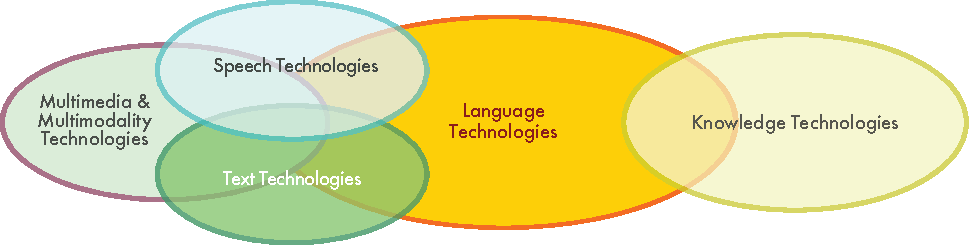
\includegraphics[width=\textwidth]{../_media/english/language_technologies}
  \caption{Language technologies}
  \label{fig:ltincontext_en}
  \colorrule{grey3}{\textwidth}{1.5pt}
\end{figure*}


Language technology is used to develop software systems designed to handle human language and are therefore often called ``human language technology''. Human language comes in spoken and written forms. While speech is the oldest and in terms of human evolution the most natural form of language communication, nonetheless complex information and much human knowledge is stored and can be transmitted through the written word. Speech and text technologies process or produce these different forms of language, and require some common resources such as dictionaries, rules of grammar, and semantics. This means that language technology (LT) links language to various forms of knowledge, independently of the media (speech or text) in which it is expressed. Figure~\ref{fig:ltincontext_en} illustrates the LT landscape.



When we communicate, we combine language with other modes of communication and information media -- for example speaking can involve gestures and facial expressions. Digital texts link to pictures and sounds. Movies may contain language in spoken and written form. In other words, speech and text technologies overlap and interact with other multimodal communication and multimedia technologies.

In this section, we will discuss the main application areas of language technology, i.\,e., language checking, web search, speech interaction, and machine translation. These applications and basic technologies include:

\begin{itemize}
\item spelling correction
\item authoring support
\item computer-assisted language learning
\item information retrieval 
\item information extraction
\item text summarisation
\item question answering
\item speech recognition 
\item speech synthesis 
\end{itemize}

Language technology is an established area of research with an extensive set of introductory literature. The interested reader is referred to the following references: \cite{carstensen-etal1, jurafsky-martin01, manning-schuetze1, lt-world1, lt-survey1}. 

Before discussing the above application areas, we will briefly describe the architecture of a typical LT system.

\subsection{Application Architectures}

Software applications for language processing typically consist of several components that mirror different aspects of language. While such applications tend to be very complex, and can be rather different for speech and text, figure~\ref{fig:textprocessingarch_en} shows a highly simplified architecture of a typical text processing system. The first three modules handle the structure and meaning of the text input:

\begin{enumerate}
\item Pre-processing: cleans the data, analyses or removes formatting, detects the input languages, replaces contractions (e.g. ``le’d thoil'' with ``le do thoil''), and so on.
\item Grammatical analysis: finds the verb, its subject and objects, modifiers and other sentence constituents; detects the sentence structure.
\item Semantic analysis: performs disambiguation (i.\,e., computes the appropriate meaning of words in a given context); resolves anaphora (i.\,e., which pronouns refer to which nouns in the sentence); represents the meaning of the sentence in a machine-readable way.
\end{enumerate}

After analysing the text, task-specific modules can perform other operations, such as automatic summarisation and database look-ups.

\begin{figure*}[htb]
  \colorrule{grey3}{\textwidth}{1.5pt}
  \center
  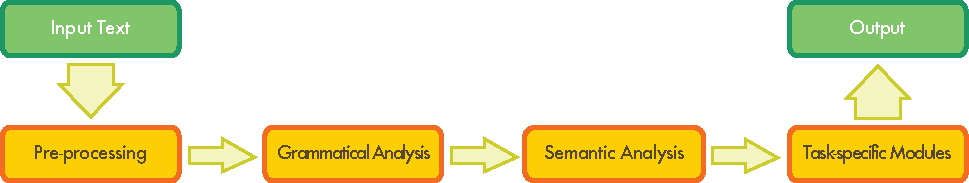
\includegraphics[width=\textwidth]{../_media/english/text_processing_app_architecture}
  \caption{A typical text processing architecture}
  \label{fig:textprocessingarch_en}
  \colorrule{grey3}{\textwidth}{1.5pt}
\end{figure*}

Speech technology applications utilise the text processing architecture outlined above. Adding speech processing to text processing requires the addition of further components. One needs models for those aspects of spoken  language not contained in text. Furthermore, working with the acoustic (speech) signal requires signal processing and speech engineering tools. Spoken language differs from text in that it contains additional layers of information, e.g., on speaker identity; physical attributes (child, adult female); origin (from the North); speaker emotion (angry, sad); attitude (friendly). In opening up access to these aspects of the information transmission which are inherent in human spoken connunication, the integration of speech processing technology with text based language technology offers particularly broad vistas for LT applications.

\begin{figure*}[hb]
  \colorrule{grey3}{\textwidth}{1.5pt}
  \center
  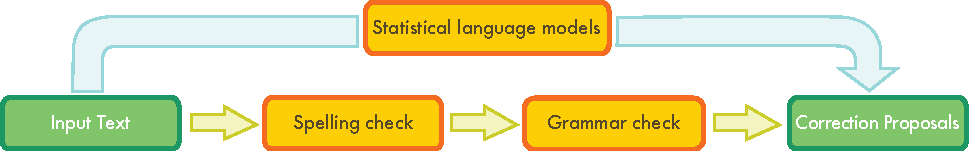
\includegraphics[width=\textwidth]{../_media/english/language_checking}
  \caption{Language checking (top: statistical; bottom: rule-based)}
  \label{fig:langcheckingaarch_en}
  \colorrule{grey3}{\textwidth}{1.5pt}
\end{figure*}

There are broadly speaking, three types of LT application architectures; those which use predominantly rule-based methods, those which use predominantly statistical (probability) based methods and hybrid systems which combine both methods. Statistical methods derive language models from  large quantities of language data (a corpus). In many cases linguistically annotated data is used or a corpus is used in conjunction with other linguistic resources such as lexicons or WordNets. The quality of the statistical model depends on the quality of the input data, therefore good quality language resources, while time consuming to create, are an essential part of the LT life-cycle. 

LT applications typically require language-specific resources such as lexicons, thesauri, semantic information, phonology, morphology and grammar rules, as well as various types of linguistically annotated corpora (both text and speech). Ideally, LT application software should be as language-independent as possible and capable of working with any language for which the relevant language-specific resources are available. In order to benefit from the most up-to-date LT applications in core areas such as machine translation, computer-aided language learning, speech  interfaces etc. it is vital that the basic language-specific resources such as those mentioned above are available. As well as corpora and linguistic data, language-specific processing tools such as morphological analysers, part-of-speech taggers and syntactic parsers  are also required. To include speech processing, further resources are needed that provide models of the sounds of the language, the intonation and rhythm, as well as resources that map from sound to text/written forms. Up-to-date theoretical and empirical linguistic research on the language is an essential prerequisite to the development of all of these language-specific resources.


In the remainder of this section, we firstly introduce the core application areas for language technology, and outline the position with regard to the Irish language in these application areas. This is followed by a brief overview of the state of LT industry, research and education in Ireland today, and a description of past and present research programmes. Finally, we present an expert estimate of core LT tools and resources for Irish in terms of various dimensions such as availability, maturity and quality. The general situation of LT for the Irish language is summarised in a matrix (figure~\ref{fig:lrlttable_en})(p.~\pageref{fig:lrlttable_en}) at the end of this section This table lists all tools and resources that are boldfaced in the text. LT support for Irish is also compared to other languages that are part of this series and finally, conclusions are drawn.

\subsection{Core Application Areas}

In this section, we focus on the most important LT tools and resources, and provide an overview of LT activities in Ireland.

\subsubsection{Language Checking}

Anyone who has used a word processor such as Microsoft Word knows that it has a spell checker that highlights spelling mistakes and proposes corrections. The first spelling correction programs compared a list of extracted words against a dictionary of correctly spelled words. Today these programs are far more sophisticated. Using language-dependent algorithms for \textbf{grammatical analysis}, they detect errors related to morphology (e.\,g., plural formation) as well as syntax-related errors, such as a missing verb or a conflict of verb-subject agreement (e.\,g., \textit{she *write a letter}). 

Tools for checking spelling are available for Irish in popular office suites such as Microsoft Office and Open Office. However Microsoft's spell checker has not been updated in many years. Currently, there is only one spell checker, GaelSpell (http://borel.slu.edu/ispell/) which is consistently updated, open source, and available for Word/OOo/Firefox, etc. There is also an open source finite-state morphological analyser and generator, a part-of-speech tagger, and a partial dependency parser (http://www.tcd.ie/slscs/itut) and an open source Irish WordNet -- Líonra Séimeantach na Gaeilge  (http://borel.slu.edu/lsg/). In addition, there are a number of stand-alone applications, including Foclóir Beag, Gléacht and EasyReader and Focal.ie which facilitate lexical and grammatical searches. 

Language checking tools check not just spelling but also many aspects of grammar. Only one language checker for Irish, An Gramadóir,  \cite{gramadoir} does more than spelling correction, and it is currently not easily integrated into either OpenOffice or Microsoft Word (though, at the time of writing, this is work in progress).


However, most spelling and grammar checkers will not find any errors in the following text \cite{zar1}:

\begin{quote}
  I have a spelling checker,\\
  It came with my PC.\\
  It plane lee marks four my revue\\
  Miss steaks aye can knot sea.
\end{quote}

Handling these kinds of errors usually requires an analysis of the context. This type of analysis either needs to draw on language-specific \textbf{grammars} laboriously coded into the software by experts, or on a statistical language model. In this case, a model calculates the probability of a particular word as it occurs in a specific position. A statistical language model can be automatically created by using a large amount of (annotated) language data (called a \textbf{text corpus}). 

\boxtext{Language checking is not limited to word processors but also applies to authoring systems.}

Both of the above approaches have been developed around data from English. Currently, neither approach can transfer easily to Irish due to a lack of basic language resources. There are no sufficiently large annotated text corpora to train a statistical model, and there has been insufficient research into the encoding of linguistic knowledge in grammars. However there is ongoing research into syntactic parsing for Irish \cite{lynn2012}, \cite{elaine2010}


Besides spelling and grammar checkers and authoring support, language checking is also important in the field of computer-assisted language learning. This is an application area which would be of enormous benefit to learners of the Irish language. However, to date computer-assisted language learning for Irish remains largely underdeveloped.

\subsubsection{Web Search}

\begin{figure*}[htb]
  \colorrule{grey3}{\textwidth}{1.5pt}
  \center
  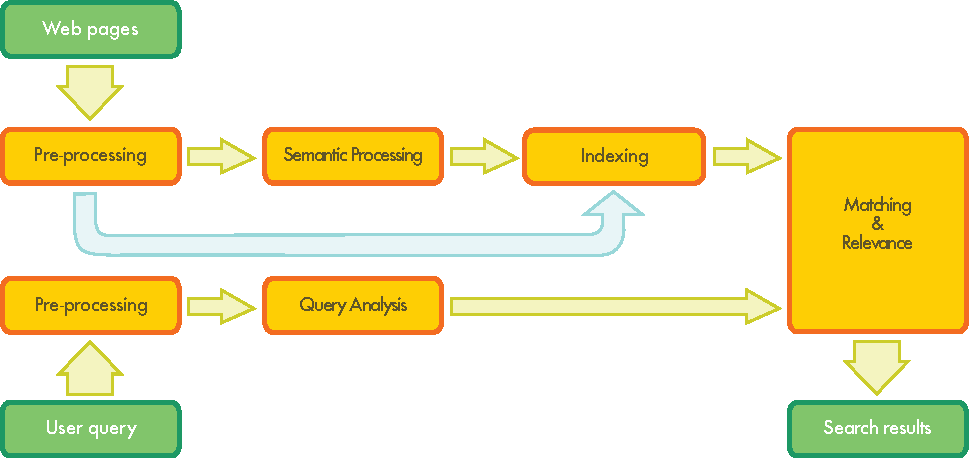
\includegraphics[width=\textwidth]{../_media/english/web_search_architecture}
  \caption{Web search architecture}
  \label{fig:websearcharch_en}
  \colorrule{grey3}{\textwidth}{1.5pt}
 \end{figure*}

Searching the Web, intranets or digital libraries is probably the most widely used yet largely underdeveloped language technology application today. The Google search engine, which started in 1998, now handles about 80\% of all search queries and over 90\% of all search queries from internet users in Ireland \cite{googlemarketshare}. As of the time of writing there is not yet an official Irish equivalent of the verb ``to google'' as there is in for example, in German. But certainly in the vernacular where, English loan words first creep into the language the term ``googláil/gúgláil'' \cite{kilgarriff2010} is used. The Google search interface and results page display has not significantly changed since the first version. Yet in the current version, Google offers spelling correction for misspelled words (but not for Irish) and has now incorporated basic semantic search capabilities that can improve search accuracy by analysing the meaning of terms in a search query context \cite{googlesemsearch}.  The Google success story shows that a large volume of available data and efficient indexing techniques can deliver satisfactory results for a statistically-based approach. 

For more sophisticated information requests, it is essential to integrate deeper linguistic knowledge to facilitate text interpretation. Experiments using \textbf{lexical resources} such as machine-readable thesauri or ontological language resources (e.g., WordNet for English or Líonra Séimeantach na Gaeilge for Irish) have demonstrated improvements in finding pages using synonyms of the original search terms, such as \textit{fuinnimh adamach} [atomic energy], \textit{cumhacht núicléach} [nuclear energy], or even more loosely related terms. 

The next generation of search engines will have to include much more sophisticated language technology, especially to deal with search queries consisting of a question or other sentence type rather than a list of keywords. For the query, \textit{Give me a list of all companies that were taken over by other companies in the last five years}, a syntactic as well as \textbf{semantic analysis} is required. The system also needs to provide an index to quickly retrieve relevant documents. A satisfactory answer will require syntactic parsing to analyse the grammatical structure of the sentence and determine that the user wants companies that have been acquired, rather than companies that have acquired other companies. For the expression \textit{last five years}, the system needs to determine the relevant range of years, taking into account the present year. The query then needs to be matched against a huge amount of unstructured data to find the pieces of information that are relevant to the user's request. This process is called information retrieval, and involves searching and ranking relevant documents. To generate a list of companies, the system also needs to recognise a particular string of words in a document represents a company name, using a process called named entity recognition.

\boxtext{The next generation of search engines will have to include much more sophisticated language technology.}

A more demanding challenge is to match a query in one language with documents in another language. Cross-lingual information retrieval involves automatically translating the query into all possible source languages and then translating the results back into the user's target language.

Now that data is increasingly found in non-textual formats, there is a need for services that deliver multimedia information retrieval by searching images, audio files and video data. In the case of audio and video files, a speech recognition module must convert the speech content into text (or into a phonetic representation) that can then be matched against a user query.

In Ireland, a number of small companies and various academic groups provide component language technologies for lexical analysis and similar tasks which could be employed in web search. A search engine for Irish, Aimsigh (http://aimsigh.com), which is tailored to the language (stemmed searches etc.) has existed since ca. 2005 -- 2006. This unfortunately has not, to date, received the attention it deserves and instead many people use Google’s Irish interface which, while localised, is not optimised or tailored to work in the language.

\subsubsection{Speech Interaction}

Speech interaction is one of many application areas that depend on speech technology, i.\,e., technologies for processing spoken language. Speech interaction technology is used to create interfaces that enable users to interact in spoken language instead of using a graphical display, keyboard and mouse.  Today, these voice user interfaces (VUI) are used for partially or fully automated telephone services provided by companies to customers, employees or partners. Business domains that rely heavily on VUIs include banking, supply chain, public transportation, and telecommunications. Other uses of speech interaction technology include interfaces to car navigation systems and the use of spoken language as an alternative to the graphical or touchscreen interfaces in smartphones.

\begin{figure*}[htb]
  \colorrule{grey3}{\textwidth}{1.5pt}
  \center
  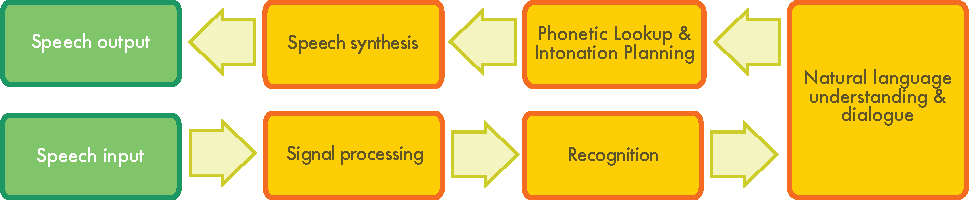
\includegraphics[width=\textwidth]{../_media/english/simple_speech-based_dialogue_architecture}
  \caption{Speech-based dialogue system}
  \label{fig:dialoguearch_en}
  \colorrule{grey3}{\textwidth}{1.5pt}
\end{figure*}

Speech interaction technology comprises four technologies: 

\begin{enumerate}
\item Automatic \textbf{speech recognition} (ASR) determines which words are actually spoken in a given sequence of sounds uttered by a user.  
\item Natural language understanding analyses the syntactic structure of a user's utterance and interprets it according to the system in question.
\item Dialogue management determines which action to take given the user input and system functionality.   
\item \textbf{Speech synthesis} (text-to-speech or TTS) transforms the system's reply into sounds for the user.
\end{enumerate}

One of the major challenges of ASR systems is to accurately recognise the words a user utters. This means restricting the range of possible user utterances to a limited set of keywords, or manually creating language models that cover a large range of natural language utterances. Using machine learning techniques, language models can also be generated automatically from \textbf{speech corpora}, i.\,e., large collections of speech audio files and text transcriptions. Restricting utterances usually forces people to use the voice user interface in a rigid way and can damage user acceptance; but the creation, tuning and maintenance of rich language models will significantly increase costs. VUIs that employ language models and initially allow a user to express their intent more flexibly -- prompted by a \textit{How may I help you?} greeting -- tend to be automated and are better accepted by users.

Companies tend to use utterances pre-recorded by professional speakers for generating the output of the voice user interface. For static utterances where the wording does not depend on particular contexts of use or personal user data, this can deliver a rich user experience. But more dynamic content in an utterance may suffer from unnatural intonation because different parts of audio files have simply been strung together. Through optimisation, today's TTS systems are getting better at producing natural-sounding dynamic utterances.

\boxtext{Speech interaction is the basis for interfaces that allow a user to interact with spoken language.}

Interfaces in speech interaction have been considerably standardised during the last decade in terms of their various technological components. There has also been strong market consolidation in speech recognition and speech synthesis. The national markets in the G20 countries (economically resilient countries with high populations) have been dominated by just five global players, with Nuance (USA) and Loquendo (Italy) being the most prominent players in Europe. In 2011, Nuance announced the acquisition of Loquendo, which represents a further step in market consolidation.

%\subsubsection*{Speech synthesis and Recognition}

Speech interaction systems depend crucially on the core technologies of \textbf{speech synthesis and recognition}. These in turn require a plethora of speech processing tools and resources which are not normally part of text processing systems. For example, to produce a speech synthesiser a corpus of spoken language is needed which has been phonetically transcribed and segmented. Pronunciation dictionaries, letter to sound rules, models of the sounds of the language, intonation models, models of the timing and rhythmic properties are also needed. Establishing speech technology for a new language thus relies on considerable prior quantitative analysis and resource building for the spoken language. 

The development of Irish synthesis (ABAIR project) is an active area of research at An tIonad do Theicneolaíocht Urlabhra agus Teangeolaíochta na Gaeilge, (ITUT), the Centre for Speech and Language Technology for Irish in TCD (\cite{pittsburgh}).  As the necessary speech resources for the language were mostly lacking for Irish a great deal of the research is concerned with putting these in place. Machine learning approaches can often offer a quick route to the development of resources in a new language. However, given the particular challenges presented by Irish (see Section~\ref{AboutIrish_en}) such approaches have tended not to work, and hand written rule-based systems have generally been required. As explained in Section~\ref{IrishInfso_en}, the technology needs to be sensitive to the language and linguistic context. In the case of Irish, a multi-dialect facility was deemed essential from the outset. With this in mind, resources are being consequently developed, where possible, with `global’ components (capturing cross-dialect common features) and `local' ones (for aspects that are dialect-specific). This design feature ensures that modules are maximally reusable, and makes the provision of resources in a new dialect much simpler.

A text-to-speech facility, the ABAIR system, has been made available on the web at www.abair.ie, for the Northern dialect of Donegal. A second voice, for the Connemara dialect will soon be made available on the same site and research on the dialect of Kerry is under way. These latter dialects are essential to cater for speakers of Southern varieties of the language.  
Although not advertised, and as yet catering for only the most northern dialect, www.abair.ie is already having an impact in the Irish speaking community both nationally and internationally. There were 40,000 hits in 2011, of which half were from outside of Ireland. It is increasingly being used in schools, particularly in Northern Ireland, where the northern dialect is suited. Teachers, parents and learners are using it: quite simply hearing how a text is spoken helps overcome two specific difficulties for learners of Irish. Firstly, as the writing system is very complex, and as the pronunciation is in any case very different from English, it can be difficult for the learner to know how written words are pronounced. Secondly, most learners, in Ireland and abroad, do not have ready access to native speakers of the language. 

Responding to a high level of interest from educationalists a synthesis based aid to literacy and pronunciation training for Irish is being developed. In collaboration with other research groups at TCD (\cite{slate2011}) the ABAIR voices are also being used to develop interactive adaptive language learning games, as well as teaching materials that exploit virtual reality scenes. The ABAIR group’s research is also urgently targeting the needs of the visually impaired, for whom synthesis provides the only way to access web or computer based materials, essential to learning Irish, to participating in education through Irish and in many aspects of the life of the Irish speaking community.

Despite the considerable progress to date, a great deal of consolidation and further development is still required to bring the corpora, the synthetic voices, the ancillary resources and technology applications up to the standard that is available for the major languages.

In the area of automatic speech recognition there has been no development to date for Irish. However, many of the resources which are being developed for synthesis are also crucial for speech recognition, and to that extent, the foundations for this aspect of technological development are being laid. It should be noted that preparation of large and diverse phonetically labelled speech corpora will be needed to further this core technology. Clearly, there is a long way to go before speech interaction systems can be put in place for Irish. While parts of the jigsaw are being gradually put in place, other crucial parts such as recognition systems need to be developed from scratch.

For the moment, speech technology for Irish involves largely PC based applications, although some mobile applications exist. Looking ahead, there will be significant changes, due to the spread of smartphones as a new platform for managing customer relationships, in addition to fixed telephones, the Internet and e-mail. This will also affect how speech interaction technology is used. In the long term, there will generally be fewer telephone-based VUIs, and spoken language apps will play a far more central role as a user-friendly input for smartphones. This will be largely driven by stepwise improvements in the accuracy of speaker-independent speech recognition via the speech dictation services already offered as centralised services to smartphone users.

\subsubsection{Machine Translation}

The idea of using digital computers to translate natural languages can be traced back to 1946 and was followed by substantial funding for research during the 1950s and again in the 1980s. 
Yet machine translation (MT) still cannot deliver on its initial promise of providing across-the-board automated translation.  

\boxtext{At its basic level, Machine Translation simply substitutes words in one natural language with words in another language.}

The most basic approach to machine translation is the automatic replacement of the words in a text written in one natural language with the equivalent words of another language. This can be useful in subject domains that have a very restricted, formulaic language such as weather reports. However, in order to produce a good translation of less restricted texts, larger text units (phrases, sentences, or even whole passages) need to be matched to their closest counterparts in the target language. The major difficulty is that human language is ambiguous. Ambiguity creates challenges on multiple levels, such as word sense disambiguation at the lexical level (a \textit{jaguar} is a brand of car or an animal) or the assignment of case on the syntactic level.

One way to build an MT system is to use linguistic rules. For translations between closely related languages, a translation using direct substitution may be feasible in cases such as the above example. However, rule-based (or linguistic knowledge-driven) systems often analyse the input text and create an intermediary symbolic representation from which the target language text can be generated. The success of these methods is highly dependent on the availability of extensive lexicons with morphological, syntactic, and semantic information, and large sets of grammar rules carefully designed by skilled linguists. This is a very long and therefore costly process.

\begin{figure*}[htb]
  \colorrule{grey3}{\textwidth}{1.5pt}
  \center
  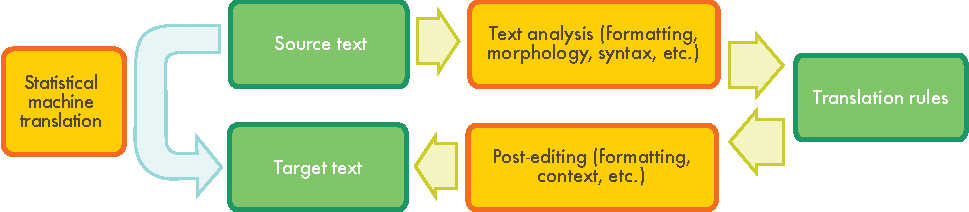
\includegraphics[width=\textwidth]{../_media/english/machine_translation}
  \caption{Machine translation (left: statistical; right: rule-based)}
  \label{fig:mtarch_en}
  \colorrule{grey3}{\textwidth}{1.5pt}
\end{figure*}

In the late 1980s when computational power increased and became cheaper, interest in statistical models for machine translation began to grow. Statistical models are derived from analysing bilingual text corpora, \textbf{parallel corpora}, such as the Europarl parallel corpus, which contains the proceedings of the European Parliament in 21 European languages. Given enough data, statistical MT works well enough to derive an approximate meaning of a foreign language text by processing parallel versions and finding plausible patterns of words. Unlike knowledge-driven systems, however, statistical (or data-driven) MT systems often generate ungrammatical output. Data-driven MT is advantageous because less human effort is required, and it can also cover special particularities of the language (e.\,g., idiomatic expressions) that are often ignored in knowledge-driven systems. 

\boxtext{Machine Translation is particularly challenging for the Irish language due to a lack of resources.}

The strengths and weaknesses of knowledge-driven and data-driven machine translation tend to be complementary, so that nowadays researchers focus on hybrid approaches that combine both methodologies. One such approach uses both knowledge-driven and data-driven systems, together with a selection module that decides on the best output for each sentence. However, results for sentences longer than, say, 12 words, will often be far from perfect. A more effective solution is to combine the best parts of each sentence from multiple outputs; this can be fairly complex, as corresponding parts of multiple alternatives are not always obvious and need to be aligned. 

Pioneering work for Irish has been done in the area of translation memories in conjunction with Foras na Gaeilge. But there is still a great deal of work to be done developing and improving the quality of MT systems for Irish. The challenges involve adapting language resources to a given subject domain or user area, and integrating the technology into workflows that already have term bases and translation memories. Another problem is that most of the current systems are English-centred and only support a few languages from and into Irish. This leads to friction in the translation workflow and forces MT users to learn different lexicon coding tools for different systems.

Some industrial development of machine translation systems for Irish has been done by Traslan Teoranta, which was recently acquired by UK-based Applied Language Solutions. In addition, the popular Google Translate engine offers functionality for working with Irish. The further development and quality of industrial MT systems for Irish is significantly affected by the lack of appropriate data and resources (e.g. parallel corpora and bilingual lexicons) which are needed to develop such systems.

Evaluation campaigns help to compare the quality of MT systems, their approaches and the status of the systems for different language pairs. Figure~\ref{fig:euromatrix_de} (p.~\pageref{fig:euromatrix_de}), which was prepared during the Euromatrix+ project, shows the pairwise performances obtained for 22 of the 23 official EU languages (Irish was not included in the comparison due to a lack of available tools). 

The results are ranked according to a BLEU score, which indicates higher scores for better translations \cite{bleu1}. A human translator would normally achieve a score of around 80 points. The best results (in green and blue) were achieved by languages that benefit from a considerable research effort in coordinated programmes and the existence of many parallel corpora (e.\,g., English, French, Dutch, Spanish and German). The languages with poorer results are shown in red. These languages either lack such development efforts or are structurally very different from other languages (e.\,g., Hungarian, Maltese and Finnish).

\subsection{Other Application Areas}

Building language technology applications involves a range of subtasks that do not always surface at the level of interaction with the user, but they provide significant service functionalities ``behind the scenes'' of the system in question. They all form important research issues that have now evolved into individual sub-disciplines of computational linguistics. 

Question answering, for example, is an active area of research for which annotated corpora have been built and scientific competitions have been initiated. The concept of question answering goes beyond keyword-based searches (in which the search engine responds by delivering a collection of potentially relevant documents) and enables users to ask a concrete question to which the system provides a single answer. For example:

\begin{itemize}
\item[] \textit{Question: How old was Neil Armstrong when he stepped on the moon?}
\item[] \textit{Answer: 38.}
\end{itemize}

While question answering is obviously related to the core area of web search, it is nowadays an umbrella term for such research issues as which different types of questions exist, and how they should be handled; how a set of documents that potentially contain the answer can be analysed and compared (do they provide conflicting answers?); and how specific information (the answer) can be reliably extracted from a document without ignoring the context. Question answering is in turn related to information extraction (IE), an area that was extremely popular and influential when computational linguistics took a statistical turn in the early 1990s. IE aims to identify specific pieces of information in specific classes of documents, such as the key players in company takeovers as reported in newspaper stories. Another common scenario that has been studied is reports on terrorist incidents. The task here consists of mapping appropriate parts of the text to a template that specifies the perpetrator, target, time, location and results of the incident. Domain-specific template-filling is the central characteristic of IE, which makes it another example of a ``behind the scenes'' technology that forms a well-demarcated research area, which in practice needs to be embedded into a suitable application environment. 

\boxtext{Language technology applications often provide significant service functionalities behind the scenes of larger software systems.}

Text summarisation and \textbf{text generation} are two areas that can act either as standalone applications or play a supporting role. Summarisation attempts to give the essentials of a long text in a short form, and is one of the features available in Microsoft Word. It mostly uses a statistical approach to identify the ``important'' words in a text (i.\,e., words that occur very frequently in the text in question but less frequently in general language use) and determine which sentences contain the most of these ``important'' words. These sentences are then extracted and put together to create the summary. In this very common commercial scenario, summarisation is simply a form of sentence extraction, and the text is reduced to a subset of its sentences. An alternative approach, for which some research has been carried out, is to generate brand new sentences that do not exist in the source text. 

\boxtext{For the Irish language, research in most text technologies is much less developed than for most European languages.}

This requires a deeper understanding of the text, which means that so far this approach is far less robust. On the whole, a text generator is rarely used as a stand-alone application but is embedded into a larger software environment, such as a clinical information system that collects, stores and processes patient data. Creating reports is just one of many applications for text summarisation. 

For the Irish language, research in these text technologies is much less developed than for other European languages. Question answering, information extraction, and summarisation have been the focus of numerous open competitions in the USA since the 1990s, primarily organised by the government-sponsored organisations DARPA and NIST. These competitions have significantly improved the start-of-the-art, but their focus has mostly been on the English language. As a result, the annotated corpora and other special resources needed to perform these tasks in other languages are not as well developed. While some exist for better resourced European languages such as German, virtually none of the necessary tools and resources are available for Irish.

\subsection{Language Technology Industry and Programmes}

User and provider industries exist for Irish LT but they are largely focused around localisation and translation services as a result of the Languages Act and the fact that Irish has become an official EU language. There is also a growing market in education as teaching practice embraces new technologies. Likewise, among the younger generations there is an emerging trend towards for the need for improved LT support for Irish.

The language industry is a significant employer in Ireland. Growing from approximately 4--5k jobs in the mid 90’s to over 12k at the turn of the century. Currently this has levelled off somewhat with estimates of around 14--16k direct jobs in the localisation and translation industry in Ireland. The Official Language Act is currently under review and the result of this review may hold implications for the translation sector and associated technologies.

There are several excellent centres for linguistics and language technology research and industrial development, for example Microsoft, IBM, Google, and Symantec all have a presence in Ireland working to some degree with various aspects of LT. But very little work is done on Irish language data by these companies. Similarly, although Government agencies such as SFI and IRCSET have invested heavily in LT related research, little of this has been research on Irish LT. This lack of investment is a result of insufficient planning for the kinds of empirical linguistic research that are needed if Irish speech and language technology is to emerge. 

Nevertheless, Irish has received some funding over the years from the EU and Irish government agencies such Foras na Gaeilge and An Chomhairle um Oideachas Gaeltachta agus Gaelscolaíochta which has enabled research and developments in the area of speech resources and synthesis technology for Irish dialects, corpus development (Nua Chorpas na hÉireann -- corpas.focloir.ie, Corpais GaLa and Abair) and text analysis tools (www.tcd.ie/slscs/itut), lexical databases (Focal.ie) and currently  a new electronic English-Irish dictionary (www.focloir.ie)  is being developed . It should also be mentioned that individuals living outside of Ireland have also contributed significantly with their own time and funds on applications such as WinGléacht, EasyReader, An Gramadóir and others.

A number of SME's have appeared: for example, one such company, Maithú, has produced a mobile phone dictionary application, which uses text-to-speech synthesis (Abair.ie). As mobile and social network markets grow, the opportunity for businesses to provide such language technologies for Irish will also receive a boost.

Despite the strong employment figures for the language industry in Ireland and growing opportunities in the domestic market for the Irish language, much of the work of LT is ``hidden'' from the end user/consumer. Many would argue this is as it should be as LT is very much an enabling technology providing components to simplify, improve or revolutionise how we interact with other products and services. For example, we do not think about what goes on in the components of our car engines, we are just happy that they work well. However, this situation creates difficulties for the LT community in that it becomes difficult to communicate to many groups the benefits and demands for language technologies. This in turn leads to a situation where many people working in related fields (e.g. car manufacturers) find it hard to see the benefit of using LT in their field.

A market exists for Irish language technologies, as can be seen from the positive response to recent web based systems (abair.ie, focal.ie), and further requests that are coming from the public, from the Irish medium education sector for language technology support across the entire curriculum,  from the wider educational sector for computer-aided language learning applications for Irish, and in particular from the visually impaired for speech synthesis. 

We can expect the demand to grow, as mature language technology services become a staple of the modern lifestyle. With the growth of online activities, specifically social networking and learning activities, the demand is likely to keep growing  driven by the increasing number  of young Irish speakers, who are usually early adopters of such technologies. This is being facilitated by the huge growth in ICT in Ireland and recent improvements in broadband infrastructure to support this.


\subsection{Language Technology Research and Education in Ireland}

\subsubsection{Research}

The Irish third level institutions, particularly in Dublin, have a strong tradition in computational linguistics and speech engineering. There is a lot of interaction and cooperation between institutes and industry partners in order to keep the field alive in Ireland. In recent years, large scale funding has been provided by Science Foundation Ireland for a cross-institutional (DCU, UCD, TCD, UCL) research cluster, the Centre for Next Generation Localisation (CNGL), which also has numerous industrial partners. Both Irish and international researchers present their work at the Dublin Computational Linguistics Research Seminar series, which  rotates annually between several third level institutions (DCU, TCD, UCD, DIT). 

With such expertise available in Irish institutions it stands out that the situation for language technologies for Irish is not better, although the potential is enormous. 

In Dublin City University there is the National Centre for Language Technology which is well established and has strong links with industrial R\&D both locally and abroad, as well as strong ties with other European centres of excellence in the field. In Trinity College Dublin, the research centre An tIonad do Theicneolaíocht Urlabhra agus Teangeolaíochta na Gaeilge (Centre for Speech and Language Technology for Irish) focuses on research and development in speech and language technology specifically for the Irish language. UCD’s Dept of Computer Science and Informatics has a particular focus on speech engineering.


Although machine translation and multilingual LT resources are major themes in the large CNGL research cluster, little of its research has focussed on Irish. This underscores the broader reality: research funding is primarily driven by the underlying goal of future economic gain, in the form of business and jobs and ultimately wealth creation. Irish, as a lesser used language does not represent a large market of significance in comparison to English, German and other European languages with greater numbers of speakers and users.

However, the ITUT group in TCD which does focus on Irish LT has made considerable progress towards developing resources for speech processing, text-to-speech synthesis, corpus development and text processing tools for Irish. This research is being carried out in a way that acknowledges and addresses the particular challenges of providing this technology in the minority language context of Irish. Along with the development of the basic resources and tools there is parallel exploration of potential applications which are already impacting in the world of the Irish language user. This latter aspect is important and is facilitated by the fact that the group includes senior academics working at the cutting edge of speech engineering, education policy, pedagogy for Irish, and disability.  It also has strong links with other research groups in TCD (e.g. Computational Linguistics Group), as well as a tradition of collaboration with other speech and language groups in Ireland and abroad.

While events exist for the research centres mentioned above along with some university events there is no conference or community event dedicated to Irish LT.


\subsubsection{Education}
There is currently only one undergraduate degree in computational linguistics available at an Irish university. The B.A. (Mod.) in Computer Science  and Language in Trinity College Dublin combines studies in computer science, linguistics and a language. This degree course can take up to  25 students per year, up to five of whom can study Irish. TCD also has a postgraduate M.Phil in Speech and Language Processing. This taught masters course offers graduates from various backgrounds (such as engineering, computing, and linguistics) an opportunity to acquire skills necessary to undertake the kind of technology-oriented research that is required for Irish LT development.  

While these taught programmes at TCD offer a foundation in the technical skills, they are taken by a very few Irish speakers. Consequently, there is a very small pool of appropriately skilled graduates entering the workforce through the Irish education system. Research in Irish LT has been hampered by the difficulty in finding suitably skilled researchers who have a high level of competence in Irish, linguistics, and engineering or computational techniques. However the few such graduates that have emerged from these courses with a high level of skills in Irish have been a vital resource in the projects carried out so far. The challenge in the sphere of education will be to find ways of ensuring that students with a high level of competence and interest in Irish are attracted into these courses with native speakers of the language being a particularly important resource. 



\subsection{Availability of Tools and Resources}

Figure~\ref{fig:lrlttable_en} provides a rating for language technology support for the Irish language. This rating of existing tools and resources was generated by leading experts in the field who provided estimates based on a scale from 0 (very low) to 6 (very high) using seven criteria.

The key results for Irish language technology can be summed up as follows:

\begin{itemize}
\item There are relatively few tools and resources available for Irish, although some areas are more advanced than others. 
\item There has been relative little and only sporadic State support to date for the research and development needed for Irish language technology development, despite robust levels of funding for LT generally.
\item In the text processing area there has been some progress, such as development of morphological and grammatical analysers, spellcheckers as well as resources such corpora and lexica.
\item In recent years there has been considerable progress towards the provision of speech synthesis and speech resources. 
\item It is important that the speech and language developments address  the challenges that are specific to Irish and the Irish language context. 
\item It is also important in the case of Irish that the user applications which are developed are those which will have maximum impact on the Irish language community, a community with a relatively small base of native speakers, a large base of learners, and a substantial speaker/learner base outside the country. 
\item Consolidation and sustainability are crucial challenges for future development. 
\item The provision of LT technology depends on the prior development of resources and tools for the language. For this, substantial investment in empirical and theoretical research is required.
\item A skilled workforce is a major challenge. There is a need to ensure that competent Irish speakers are attracted into the foundation courses that are available.
\end{itemize}


\begin{figure*}[htb]
\centering
%\begin{tabular}{>{\columncolor{orange1}}p{.33\linewidth}ccccccc} % ORIGINAL
\begin{tabular}{>{\columncolor{orange1}}p{.33\linewidth}@{\hspace*{6mm}}c@{\hspace*{6mm}}c@{\hspace*{6mm}}c@{\hspace*{6mm}}c@{\hspace*{6mm}}c@{\hspace*{6mm}}c@{\hspace*{6mm}}c}
\rowcolor{orange1}
 \cellcolor{white}&\begin{sideways}\makecell[l]{Quantity}\end{sideways}
&\begin{sideways}\makecell[l]{\makecell[l]{Availability} }\end{sideways} &\begin{sideways}\makecell[l]{Quality}\end{sideways}
&\begin{sideways}\makecell[l]{Coverage}\end{sideways} &\begin{sideways}\makecell[l]{Maturity}\end{sideways} &\begin{sideways}\makecell[l]{Sustainability}\end{sideways} &\begin{sideways}\makecell[l]{Adaptability}\end{sideways} \\ \addlinespace
\multicolumn{8}{>{\columncolor{orange2}}l}{Language Technology: Tools, Technologies and Applications} \\ \addlinespace
Speech Recognition	&0&0&0&0&0&0&0 \\ \addlinespace
Speech Synthesis &3&3&3&3&2&1&2\\ \addlinespace
Grammatical analysis &4&4&3&3&4&4&4\\ \addlinespace %
Semantic analysis &2&2&0&0&2&2&1\\ \addlinespace %
Text generation &1&0&1&1&1&1&1\\ \addlinespace %
Machine translation &2&3&1&1&1&1&1\\ \addlinespace %
\multicolumn{8}{>{\columncolor{orange2}}l}{Language Resources: Resources, Data and Knowledge Bases} \\ \addlinespace
Text corpora &3&4&3&3&4&3&3\\ \addlinespace %
Speech corpora &1&2&3&1&3&3&3\\ \addlinespace %
Parallel corpora &2&3&2&2&3&2&3\\ \addlinespace %
Lexical resources &4&3&4&3&3&3&3\\ \addlinespace
Grammars &1&3&3&2&2&2&2\\
\end{tabular}
\caption{State of language technology support for Irish}
\label{fig:lrlttable_en}
\end{figure*}

The results show that there is limited technological support for Irish and that the basic linguistic resources to support the development of core technologies are largely absent. It is clear that when investments in such tools and resources are made that quality tools and resources can be created.

\subsection{Cross-language comparison}
The current state of LT support varies considerably from one language community to another. In order to compare the situation between languages, this section will present an evaluation based on two sample application areas (machine translation and speech processing) and one underlying technology (text analysis), as well as basic resources needed for building LT applications. The languages were categorised using the following five-point scale: 

\begin{enumerate}
\item Excellent support
\item Good support
\item Moderate support
\item Fragmentary support
\item Weak or no support
\end{enumerate}

Language Technology support was measured according to the following criteria:

\textbf{Speech Processing:} Quality of existing speech recognition technologies, quality of existing speech synthesis technologies, coverage of domains, number and size of existing speech corpora, amount and variety of available speech-based applications.

\textbf{Machine Translation:} Quality of existing MT technologies, number of language pairs covered, coverage of linguistic phenomena and domains, quality and size of existing parallel corpora, amount and variety of available MT applications.

\textbf{Text Analysis:} Quality and coverage of existing text analysis technologies (morphology, syntax, semantics), coverage of linguistic phenomena and domains, amount and variety of available applications, quality and size of existing (annotated) text corpora, quality and coverage of existing lexical resources (e.\,g., WordNet) and grammars.

\textbf{Resources:} Quality and size of existing text corpora, speech corpora and parallel corpora, quality and coverage of existing lexical resources and grammars.

Figures~\ref{fig:speech_cluster_en} to~\ref{fig:resources_cluster_en} show that in each cross-language comparison of application areas,  Irish falls into category 4: Fragmentary Support or category 5: Weak or no support. Overall, this presents a picture of Irish as not being very well equipped with language technologies or language resources. 

In Figure~\ref{fig:speech_cluster_en}, Speech processing for Irish is shown as having ``fragmentary support''. However, there are some green shoots. Important advances have been made in recent years towards the provision of speech processing technologies and resources. With consolidation and expansion this area could well yield major dividends in technologies and applications. Speech applications are particularly crucial supports for Irish as a minority language in modern Ireland: by extending the use of the spoken language, by supporting the learning of Irish, by opening Irish to those for whom access is difficult (e.g. those with visual and vocal disabilities, those living abroad or in communities where there is little access to native speakers), and even by virtue of the fact that they may provide ``virtual'' speakers even of endangered dialects, they could and should play a role in the maintenance and preservation of the language. 

In Figure~\ref{fig:mt_cluster_en}, Machine Translation for Irish is shown as having ``weak or no support''. While machine translation (MT) has good or moderate support for other European languages, the transfer of technology to Irish is hampered by the lack of language specific resources for Irish. In the case of both statistical MT systems (e.g. Moses) and rule-based MT sytems (e.g. Moses, Apertium) applications for Irish cannot be developed  without the availability of language specific resources for source and target languages, such as parallel corpora and bilingual lexicons,  as well as further linguistic research into Irish syntax and semantics. The necessary building blocks must be put in place in order to enable the technological development.

In Figure~\ref{fig:text_cluster_en}, Text analysis for Irish is shown as having ``weak or no support''. While there is good support for morphological analysis, syntactic and semantic analysis is at a much earlier stage of development. In the area of syntax, basic linguistic research on the linguistic phenomena of Irish syntax is required. There is also much work to be done in the area of semantics, such as semantic roles and valencies for verbs and semantic classes for nouns. While there is ongoing research in all of these areas it is somewhat fragmented, therefore the establishment of  Irish Network in Formal Linguistics (http://linguisticsnet.wordpress.com/) is a welcome development, particularly as one of its stated aims is ``to encourage and develop research on the linguistics of Irish''.


In Figure~\ref{fig:resources_cluster_en}, Speech and text resources for Irish in comparison to other European languages is shown as having ``weak or no support''. Speech corpora (phonetically balanced high quality recordings required for speech synthesis), and other resources required for speech technology are being developed as part of the ABAIR synthesis  project. These include intonation models, letter-to-sound rules, pronunciation lexica etc, and particular attention is being given to the need to cater for the various dialects.  In the area of text processing, there is a 30 million word corpus of written text (NCI) which is part-of-speech tagged. While  parallel corpora (Irish, English) exist (\cite{scannell}, http://www.focal.ie/ParaDocs.aspx) the domains are mostly limited to EU parliamentary debates, Irish legislation and other web texts. In order to support the development of MT and other applications these parallel corpora need to be extended to include more topics and genres. In addition to written texts there is a need for a comprehensive corpus of spoken Irish to enable linguistic research, and the development of CALL applications and speech recognition. The GaLa project (http://www.tcd.ie/slscs/itut) has recently initiated work on a diachronic corpus of spoken Irish.

However, the clustering across languages shows that Irish is not alone in lagging behind in the provision of these technologies and resources. Many other European languages are facing similar difficulties.  Key differentiating factors, though, are that most of these other languages have much higher numbers of speakers; they are not competing on the ground with a much better resourced language like English; and they are not minority languages in the regions where they are spoken. Furthermore, most of the other languages do not have to contend with the specific challenges both linguistic and sociolinguistic in nature, that pertain in the case of Irish. It is also clear that the development of LT for Irish cannot be left to market forces and the Irish government must take a proactive role in promoting LT development.

Looking at the tables in this light we can see that without making some drastic changes Irish is very much at risk of being left behind other languages as Language Technology advances are made. This is a serious situation for Ireland both politically and socially. Fortunately, Ireland still has a strong indigenous language services industry and is home to several world class speech and language technology research centres. In principle, Irish could rapidly take a massive step forward into the information age, and stands to gain particularly from the technology, in a myriad of ways that would not be immediately obvious to speakers of major languages. Indeed language technology is likely to play an important role in the maintenance and preservation of the language, and in the strengthening of the Irish speaking community. Although the main benefits in the first instance will be social and cultural, the development of this technology will also bring economic benefits through employment, R\&D and a path to market. The increased enablement for Irish language speakers has the potential to make Ireland a leading light in LT development for under-resourced languages which face many of the same challenges and roadblocks. A concerted national approach encompassing research, industry and language policy will be needed to realise this goal.


\subsection{Conclusions}

\emph{In this series of white papers, we have made an important effort by assessing the language technology support between 30 European languages, and by providing a high-level comparison across these languages. By identifying the gaps, needs and deficits, the European language technology community and its related stakeholders are now in a position to design a large scale research and development programme aimed at building a truly multilingual, technology-enabled communication across Europe.}

The results of this white paper series show that there is a dramatic difference in language technology support between the various European languages. While there are good quality software and resources available for some languages and application areas, others, usually less widely spoken languages, have substantial gaps. Many languages lack basic technologies for text analysis and the essential resources. Others have basic tools and resources but the implementation of for example semantic methods is still far away. Therefore a large-scale effort is needed to attain the ambitious goal of providing high-quality language technology support for all European languages, for example through high quality machine translation. 

The EUROMAP Language Technologies \cite{euromap} project in 2003, investigated the state-of-the-art of LT research and take-up in Europe, as well as the background for the present situation in each country. The report concludes that a visible presence for European LT activities should be established for Europe, as no other advanced economic area enjoys such cultural and linguistic diversity. The goal should be to have a set of robust, stable, multilingual LT modules, capable of being embedded into emerging ICT application environments. The study also highlights some of the strengths in Ireland’s  LT R\&D provision for Irish. Based on the metrics used, Ireland falls in a group of ``promising'' countries with respect to LT R\&D but  needs considerable investment if it is to attain the standards to which we should aspire.

The issue of technology transfer, as identified by EUROMAP is a key factor in securing a place for the Irish language in the modern information society. Various social, educational and political factors in Ireland have created a strong demand for ICT in Irish due to the growing centrality of digital technology in all aspects of modern society. However, as may be clear from the foregoing, the transfer of technology to a new language is not necessarily a simple matter, and will only happen if there is serious empirical research geared towards developing the underpinning resources. The development of speech and language technology needs to be sensitive to the real needs of the language communities involved, and prioritise those aspects that are likely to have the maximum positive impact.

Ireland to date has chosen to focus its resources on building a powerful IT service industry rather than on developing a national language research base. As a result it hosts a significant concentration of language localisation expertise and research which has fuelled a strong industry around LT in the translation and localisation fields. However, they are largely focused towards supporting industrial goals. Hence, the state of the art language technologies developed in Ireland are slow in being applied to national interests and the Irish language itself.

The current situation where there is a clear and growing demand for technologies which both support and enable the Irish language represents a unique opportunity for LT research and development in Ireland. National and European initiatives and directives are creating a growing demand for translation and localisation of information, documents and services into Irish. At the same time the demand for confident and competent speakers, translators and linguists in Irish is growing. This has created a demand, and an opportunity, for the creation of state-of-the-art core LT resources for Irish, as well as the need to bridge the gap between research and the public at large by providing new and innovative applications which can support students of the language and those eager to partake in the information society through Irish. Bearing in mind the complexity of affecting technology transfer it will be important to leverage existing LTs, developed for other languages, to suit Irish. This combined with improved LT technology transfer to market will ensure a place for the Irish language in the information society.

Our findings show that the only course of action is to make a substantial effort to create LT resources for Irish, and use them to drive forward research, innovation and development. The need for large-scale resource development and the complexity of language technology systems makes it vital to develop a new infrastructure and a more coherent research organisation to spur greater sharing and cooperation. There is also a need to promote awareness among the general public of the LT applications as they are being developed.

Along with a lack of continuity in research and development funding. Short-term coordinated programmes tend to alternate with periods of sparse or zero funding. In addition, there is an overall lack of coordination with programmes in other EU countries and at the European Commission level.

Funding for Irish LT tends to fall ``between two stools''. Funding bodies for science and technology do not have a particular remit for Irish, and Irish language bodies do not have a particular remit for research funding. Where funding has been obtained for Irish LT, it has tended to be from Irish language bodies whose remit does not normally extend to supporting research and therefore the funding is limited and tends to be short-term. As a consequence researchers spend an inordinate amount of their time trying to secure continuity of funding. Though much has been achieved through such short term research projects, it is not a sustainable way to fund the kind of continuous research that is needed to provide high quality technological resources for the language. 

Short term funding is particularly problematic considering lack of suitably trained researchers with skills in Irish/linguistics as well as in the technical skills. Such expertise cannot be bought in. There is a considerable investment of time involved in training in a researcher for a project, which is wasted if these researchers are lost because of lack of continued funding. 

In the sphere of education, the challenge will be to find ways of ensuring that students with a high level of competence and interest in Irish are attracted into graduate and undergraduate courses which support LT. Native speakers of the language are a particularly important resource. Although Irish Studies in the universities tend to attract many students, the focus in these departments have tended to be more on literature, and often on historical  and cultural aspects of the language. Affirmative action will be required to attract students also into empirical linguistic studies, linked to speech and language processing for Irish.




%\begin{figure*}[htb]
%  \colorrule{grey3}{\textwidth}{1.5pt}
%  \center
%  \includegraphics[width=\textwidth]{./EuromapScorecard}
%  \caption{EUROMAP HLT Scorecard}
%  \label{fig:EuromapHLT_EN}
%  \colorrule{grey3}{\textwidth}{1.5pt}
%\end{figure*}
%NEED TO ADD DIAGRAM


We can therefore conclude that there is an urgent need for a large, coordinated initiative focused on overcoming the differences in language technology readiness for European languages as a whole.

META-NET’s long-term goal is to introduce high-quality language technology for all languages in order to achieve political and economic unity through cultural diversity. The technology will help tear down existing barriers and build bridges between Europe’s languages. This requires all stakeholders - in politics, research, business, and society - to unite their efforts for the future. A large coordinated effort focused on language technologies would help safeguard the future of the Irish language, together with other languages, and establish a genuine multilingual agenda for Europe and the world as a whole \cite{tcstar}. 



\begin{figure*}[tb]
  \small
  \centering
  \begin{tabular}
  { % defines color for each column.
  >{\columncolor{corange5}}p{.13\linewidth}@{\hspace{.040\linewidth}}
  >{\columncolor{corange4}}p{.13\linewidth}@{\hspace{.040\linewidth}}
  >{\columncolor{corange3}}p{.13\linewidth}@{\hspace{.040\linewidth}}
  >{\columncolor{corange2}}p{.13\linewidth}@{\hspace{.040\linewidth}}
  >{\columncolor{corange1}}p{.13\linewidth} 
  }
  \multicolumn{1}{>{\columncolor{white}}c@{\hspace{.040\linewidth}}}{\textbf{Excellent}} & 
  \multicolumn{1}{@{}>{\columncolor{white}}c@{\hspace{.040\linewidth}}}{\textbf{Good}} &
  \multicolumn{1}{@{}>{\columncolor{white}}c@{\hspace{.040\linewidth}}}{\textbf{Moderate}} &
  \multicolumn{1}{@{}>{\columncolor{white}}c@{\hspace{.040\linewidth}}}{\textbf{Fragmentary}} &
  \multicolumn{1}{@{}>{\columncolor{white}}c}{\textbf{Weak/no}} \\ 
  \multicolumn{1}{>{\columncolor{white}}c@{\hspace{.040\linewidth}}}{\textbf{support}} & 
  \multicolumn{1}{@{}>{\columncolor{white}}c@{\hspace{.040\linewidth}}}{\textbf{support}} &
  \multicolumn{1}{@{}>{\columncolor{white}}c@{\hspace{.040\linewidth}}}{\textbf{support}} &
  \multicolumn{1}{@{}>{\columncolor{white}}c@{\hspace{.040\linewidth}}}{\textbf{support}} &
  \multicolumn{1}{@{}>{\columncolor{white}}c}{\textbf{support}} \\ \addlinespace
  
& \vspace*{0.5mm}English
& \vspace*{0.5mm}
Czech \newline 
Dutch \newline 
Finnish \newline 
French \newline 
German \newline   
Italian \newline  
Portuguese \newline 
Spanish \newline
& \vspace*{0.5mm}Basque \newline 
Bulgarian \newline 
Catalan \newline 
Danish \newline 
Estonian \newline 
Galician\newline 
Greek \newline  
Hungarian  \newline
\textbf{Irish} \newline  
Norwegian \newline 
Polish \newline 
Serbian \newline 
Slovak \newline 
Slovene \newline 
Swedish \newline
& \vspace*{0.5mm}
Croatian \newline 
Icelandic \newline  
Latvian \newline 
Lithuanian \newline 
Maltese \newline 
Romanian\\
\end{tabular}
\caption{Speech processing: state of language technology support for 30 European languages}
\label{fig:speech_cluster_en}
\end{figure*}

\begin{figure*}[tb]
  \small
  \centering
  \begin{tabular}
  { % defines color for each column.
  >{\columncolor{corange5}}p{.13\linewidth}@{\hspace{.040\linewidth}}
  >{\columncolor{corange4}}p{.13\linewidth}@{\hspace{.040\linewidth}}
  >{\columncolor{corange3}}p{.13\linewidth}@{\hspace{.040\linewidth}}
  >{\columncolor{corange2}}p{.13\linewidth}@{\hspace{.040\linewidth}}
  >{\columncolor{corange1}}p{.13\linewidth} 
  }
  \multicolumn{1}{>{\columncolor{white}}c@{\hspace{.040\linewidth}}}{\textbf{Excellent}} & 
  \multicolumn{1}{@{}>{\columncolor{white}}c@{\hspace{.040\linewidth}}}{\textbf{Good}} &
  \multicolumn{1}{@{}>{\columncolor{white}}c@{\hspace{.040\linewidth}}}{\textbf{Moderate}} &
  \multicolumn{1}{@{}>{\columncolor{white}}c@{\hspace{.040\linewidth}}}{\textbf{Fragmentary}} &
  \multicolumn{1}{@{}>{\columncolor{white}}c}{\textbf{Weak/no}} \\ 
  \multicolumn{1}{>{\columncolor{white}}c@{\hspace{.040\linewidth}}}{\textbf{support}} & 
  \multicolumn{1}{@{}>{\columncolor{white}}c@{\hspace{.040\linewidth}}}{\textbf{support}} &
  \multicolumn{1}{@{}>{\columncolor{white}}c@{\hspace{.040\linewidth}}}{\textbf{support}} &
  \multicolumn{1}{@{}>{\columncolor{white}}c@{\hspace{.040\linewidth}}}{\textbf{support}} &
  \multicolumn{1}{@{}>{\columncolor{white}}c}{\textbf{support}} \\ \addlinespace
  
& \vspace*{0.5mm} English 
& \vspace*{0.5mm} 
French \newline 
Spanish
& \vspace*{0.5mm}
Catalan \newline 
Dutch \newline 
German \newline 
Hungarian \newline
Italian \newline 
Polish \newline 
Romanian \newline 
& \vspace*{0.5mm}Basque \newline 
Bulgarian \newline 
Croatian \newline 
Czech \newline
Danish \newline 
Estonian \newline 
Finnish \newline 
Galician \newline 
Greek \newline 
Icelandic \newline 
\textbf{Irish} \newline 
Latvian \newline 
Lithuanian \newline 
Maltese \newline 
Norwegian \newline 
Portuguese \newline 
Serbian \newline 
Slovak \newline 
Slovene \newline 
Swedish \newline 
\end{tabular}
\caption{Machine translation: state of language technology support for 30 European languages}
\label{fig:mt_cluster_en}
\end{figure*}

\begin{figure*}[tb]
  \small
  \centering
  \begin{tabular}
  { % defines color for each column.
  >{\columncolor{corange5}}p{.13\linewidth}@{\hspace{.040\linewidth}}
  >{\columncolor{corange4}}p{.13\linewidth}@{\hspace{.040\linewidth}}
  >{\columncolor{corange3}}p{.13\linewidth}@{\hspace{.040\linewidth}}
  >{\columncolor{corange2}}p{.13\linewidth}@{\hspace{.040\linewidth}}
  >{\columncolor{corange1}}p{.13\linewidth} 
  }
  \multicolumn{1}{>{\columncolor{white}}c@{\hspace{.040\linewidth}}}{\textbf{Excellent}} & 
  \multicolumn{1}{@{}>{\columncolor{white}}c@{\hspace{.040\linewidth}}}{\textbf{Good}} &
  \multicolumn{1}{@{}>{\columncolor{white}}c@{\hspace{.040\linewidth}}}{\textbf{Moderate}} &
  \multicolumn{1}{@{}>{\columncolor{white}}c@{\hspace{.040\linewidth}}}{\textbf{Fragmentary}} &
  \multicolumn{1}{@{}>{\columncolor{white}}c}{\textbf{Weak/no}} \\ 
  \multicolumn{1}{>{\columncolor{white}}c@{\hspace{.040\linewidth}}}{\textbf{support}} & 
  \multicolumn{1}{@{}>{\columncolor{white}}c@{\hspace{.040\linewidth}}}{\textbf{support}} &
  \multicolumn{1}{@{}>{\columncolor{white}}c@{\hspace{.040\linewidth}}}{\textbf{support}} &
  \multicolumn{1}{@{}>{\columncolor{white}}c@{\hspace{.040\linewidth}}}{\textbf{support}} &
  \multicolumn{1}{@{}>{\columncolor{white}}c}{\textbf{support}} \\ \addlinespace

& \vspace*{0.5mm}English
& \vspace*{0.5mm}
  Dutch \newline 
  French \newline 
  German \newline 
  Italian \newline 
  Spanish
& \vspace*{0.5mm}Basque \newline 
  Bulgarian \newline 
  Catalan \newline 
  Czech \newline 
  Danish \newline 
  Finnish \newline 
  Galician \newline 
  Greek \newline 
  Hungarian \newline 
  Norwegian \newline 
  Polish \newline 
  Portuguese \newline 
  Romanian \newline 
  Slovak \newline 
  Slovene \newline 
  Swedish \newline 
& \vspace*{0.5mm}
  Croatian \newline 
  Estonian \newline 
  Icelandic \newline 
  \textbf{Irish} \newline 
  Latvian \newline 
  Lithuanian \newline 
  Maltese \newline 
  Serbian \\
  \end{tabular}
\caption{Text analysis: state of language technology support for 30 European languages}
\label{fig:text_cluster_en}
\end{figure*}

\begin{figure*}[tb]
  \small
  \centering
  \begin{tabular}
  { % defines color for each column.
  >{\columncolor{corange5}}p{.13\linewidth}@{\hspace{.040\linewidth}}
  >{\columncolor{corange4}}p{.13\linewidth}@{\hspace{.040\linewidth}}
  >{\columncolor{corange3}}p{.13\linewidth}@{\hspace{.040\linewidth}}
  >{\columncolor{corange2}}p{.13\linewidth}@{\hspace{.040\linewidth}}
  >{\columncolor{corange1}}p{.13\linewidth} 
  }
  \multicolumn{1}{>{\columncolor{white}}c@{\hspace{.040\linewidth}}}{\textbf{Excellent}} & 
  \multicolumn{1}{@{}>{\columncolor{white}}c@{\hspace{.040\linewidth}}}{\textbf{Good}} &
  \multicolumn{1}{@{}>{\columncolor{white}}c@{\hspace{.040\linewidth}}}{\textbf{Moderate}} &
  \multicolumn{1}{@{}>{\columncolor{white}}c@{\hspace{.040\linewidth}}}{\textbf{Fragmentary}} &
  \multicolumn{1}{@{}>{\columncolor{white}}c}{\textbf{Weak/no}} \\ 
  \multicolumn{1}{>{\columncolor{white}}c@{\hspace{.040\linewidth}}}{\textbf{support}} & 
  \multicolumn{1}{@{}>{\columncolor{white}}c@{\hspace{.040\linewidth}}}{\textbf{support}} &
  \multicolumn{1}{@{}>{\columncolor{white}}c@{\hspace{.040\linewidth}}}{\textbf{support}} &
  \multicolumn{1}{@{}>{\columncolor{white}}c@{\hspace{.040\linewidth}}}{\textbf{support}} &
  \multicolumn{1}{@{}>{\columncolor{white}}c}{\textbf{support}} \\ \addlinespace
    
& \vspace*{0.5mm}English
& \vspace*{0.5mm} 
    Czech \newline 
    Dutch \newline 
    French \newline 
    German \newline 
    Hungarian \newline
    Italian \newline
    Polish \newline
    Spanish \newline
    Swedish \newline 
& \vspace*{0.5mm} Basque\newline 
    Bulgarian\newline 
    Catalan \newline 
    Croatian \newline 
    Danish \newline 
    Estonian \newline 
    Finnish \newline 
    Galician \newline 
    Greek \newline 
    Norwegian \newline 
    Portuguese \newline 
    Romanian \newline 
    Serbian \newline 
    Slovak \newline 
    Slovene \newline
&  \vspace*{0.5mm}
    Icelandic \newline 
    \textbf{Irish} \newline 
    Latvian \newline 
    Lithuanian \newline 
    Maltese  \\
  \end{tabular}
  \caption{Speech and text resources: State of support for 30 European languages}  
  \label{fig:resources_cluster_en}
\end{figure*}





\end{multicols}

\clearpage

\ssection[About META-NET]{About META-NET}

\begin{multicols}{2}
META-NET is a Network of Excellence partially funded by the European Commission \cite{rehm2011}. The network currently consists of 54 research centres in 33 European countries. META-NET forges META, the Multilingual Europe Technology Alliance, a growing community of language technology professionals and organisations in Europe. META-NET fosters the technological foundations for a truly multilingual European information society that:

\begin{itemize}
\item makes communication and cooperation possible across languages;
\item grants all Europeans equal access to information and knowledge regardless of their language;
\item builds upon and advances functionalities of networked information technology.
\end{itemize}

The network supports a Europe that unites as a single digital market and information space. It stimulates and promotes multilingual technologies for all European languages. These technologies support automatic translation, content production, information processing and knowledge management for a wide variety of subject domains and applications. They also enable intuitive language-based interfaces to technology ranging from household electronics, machinery and vehicles to computers and robots.
Launched on 1 February 2010, META-NET has already conducted various activities in its three lines of action META-VISION, META-SHARE and META-RESEARCH.

\textbf{META-VISION} fosters a dynamic and influential stakeholder community that unites around a shared vision and a common strategic research agenda (SRA). The main focus of this activity is to build a coherent and cohesive LT community in Europe by bringing together representatives from highly fragmented and diverse groups of stakeholders. The present White Paper was prepared together with volumes for 29 other languages. The shared technology vision was developed in three sectorial Vision Groups. The META Technology Council was established in order to discuss and to prepare the SRA based on the vision in close interaction with the entire LT community.

\textbf{META-SHARE} creates an open, distributed facility for exchanging and sharing resources. The peer-to-peer network of repositories will contain language data, tools and web services that are documented with high-quality metadata and organised in standardised categories. The resources can be readily accessed and uniformly searched. The available resources include free, open source materials as well as restricted, commercially available, fee-based items.

\textbf{META-RESEARCH} builds bridges to related technology fields. This activity seeks to leverage advances in other fields and to capitalise on innovative research that can benefit language technology. In particular, the action line focuses on conducting leading-edge research in machine translation, collecting data, preparing data sets and organising language resources for evaluation purposes; compiling inventories of tools and methods; and organising workshops and training events for members of the community.\\\\

\textbf{\centerline{office@meta-net.eu -- http://www.meta-net.eu}}
\end{multicols}

%META-NET is a Network of Excellence funded by the European Commission. The network currently consists of 54 members from 33 European countries \cite{rehm2011}. META-NET fosters the Multilingual Europe Technology Alliance (META), a growing community of language technology professionals and organisations in Europe. META-NET cooperates with other initiatives like the Common Language Resources and Technology Infrastructure (CLARIN), which is helping to establish digital humanities research in Europe. META-NET fosters the technological foundations for a truly multilingual European information society that:

%\begin{itemize}
%\item makes communication and cooperation possible across languages;
%\item provides equal access to information and knowledge in any language;
%\item offers advanced and affordable networked information technology to European citizens.
%\end{itemize}

%META-NET stimulates and promotes multilingual technologies for all European languages. The technologies enable automatic translation, content production, information processing and knowledge management for a wide variety of applications and subject domains. The network wants to improve current approaches, so better communication and cooperation across languages can take place. Europeans have an equal right to information and knowledge regardless of language.

%META-NET launched on 1 February 2010 with the goal of advancing research in language technology (LT). The network supports a Europe that unites as a single digital market and information space. META-NET has conducted several activities that further its goals. META-VISION, META-SHARE and META-RESEARCH are the network's three lines of action.

%\textbf{META-VISION} fosters a dynamic and influential stakeholder community that unites around a shared vision and a common strategic research agenda (SRA). The main focus of this activity is to build a coherent and cohesive LT community in Europe by bringing together representatives from highly fragmented and diverse groups of stakeholders. In the first year of META-NET, presentations at the FLaReNet Forum (Spain), Language Technology Days (Luxembourg), JIAMCATT 2010 (Luxembourg), LREC 2010 (Malta), EAMT 2010 (France) and ICT 2010 (Belgium) centred on public outreach. According to initial estimates, META-NET has already contacted more than 2,500 LT professionals to develop its goals and visions with them. At the META-FORUM 2010 event in Brussels, META-NET communicated the initial results of its vision building process to more than 250 participants. In a series of interactive sessions, the participants provided feedback on the visions presented by the network. 

%\textbf{META-SHARE} creates an open, distributed facility for exchanging and sharing resources. The peer-to-peer network of repositories will contain language data, tools and web services that are documented with high-quality metadata and organised in standardised categories. The resources can be readily accessed and uniformly searched. The available resources include free, open source materials as well as restricted, commercially available, fee-based items. META-SHARE targets existing language data, tools and systems as well as new and emerging products that are required for building and evaluating new technologies, products and services. The reuse, combination, repurposing and re-engineering of language data and tools plays a crucial role. META-SHARE will eventually become a critical part of the LT marketplace for developers, localisation experts, researchers, translators and language professionals from small, mid-sized and large enterprises. META-SHARE addresses the full development cycle of LT -- from research to innovative products and services. A key aspect of this activity is establishing META-SHARE as an important and valuable part of a European and global infrastructure for the LT community. 

%\textbf{META-RESEARCH} builds bridges to related technology fields. This activity seeks to leverage advances in other fields and to capitalise on innovative research that can benefit language technology. In particular, this activity wants to bring more semantics into machine translation (MT), optimise the division of labour in hybrid MT, exploit context when computing automatic translations and prepare an empirical base for MT. META-RESEARCH is working with other fields and disciplines, such as machine learning and the Semantic Web community. META-RESEARCH focuses on collecting data, preparing data sets and organising language resources for evaluation purposes; compiling inventories of tools and methods; and organising workshops and training events for members of the community. This activity has already clearly identified aspects of MT where semantics can impact current best practices. In addition, the activity has created recommendations on how to approach the problem of integrating semantic information into MT. META-RESEARCH is also finalising a new language resource for MT, the Annotated Hybrid Sample MT Corpus, which provides data for English-German, English-Spanish and English-Czech language pairs. META-RESEARCH has also developed software that collects multilingual corpora that are hidden on the Web.
%\end{multicols}
%\vfill
%\centerline{office@meta-net.eu -- http://www.meta-net.eu}

\cleardoublepage

\appendix
\addtocontents{toc}{\protect\bigskip}

\bsection[Tagairtí -- References]{Tagairtí --- References}
\bibliographystyle{unsrt}
\bibliography{irish_references}
  
\cleardoublepage

\bsection[META-NET Eagraíochtaí atá ina mBaill -- META-NET Members]{META-NET Eagraíochtaí atá ina mBaill --- META-NET Members}
\label{metanetmembers}

\small
\begin{longtable}{@{}llp{113mm}@{}}
  an Bheilg & \textcolor{grey1}{Belgium} & Computational Linguistics and Psycholinguistics Research Centre, University of Antwerp: Walter Daelemans\\ \addlinespace
  & & Centre for Processing Speech and Images, University of Leuven: Dirk van Compernolle \\ \addlinespace
  
  an Bhulgáir & \textcolor{grey1}{Bulgaria} & Inst. for Bulgarian Language, Bulgarian Academy of Sciences: Svetla Koeva \\ \addlinespace
  
  an Chipir & \textcolor{grey1}{Cyprus} & Language Centre, School of Humanities: Jack Burston \\ \addlinespace
  
  an Chróit & \textcolor{grey1}{Croatia} & Inst. of Linguistics, Faculty of Humanities and Social Science, University of Zagreb: Marko Tadić \\ \addlinespace
  
  an Danmhairg &  \textcolor{grey1}{Denmark} & Centre for Language Technology, University of Copenhagen: \newline Bolette Sandford Pedersen, Bente Maegaard\\ \addlinespace
  
  an Eastóin & \textcolor{grey1}{Estonia} & Inst. of Computer Science, University of Tartu: Tiit Roosmaa, Kadri Vider\\ \addlinespace
  
  an Eilvéis & \textcolor{grey1}{Switzerland} & Idiap Research Inst.: Hervé Bourlard \\ \addlinespace
  
  Éire & \textcolor{grey1}{Ireland} & School of Computing, Dublin City University: Josef van Genabith\\ \addlinespace
  
  an Fhionlainn  & \textcolor{grey1}{Finland} & Computational Cognitive Systems Research Group, Aalto University: Timo Honkela\\ \addlinespace
  & & Dept. of Modern Languages, University of Helsinki: Kimmo Koskenniemi,\newline Krister Lindén \\ \addlinespace
  
  an Fhrainc & \textcolor{grey1}{France} & Centre National de la Recherche Scientifique, Laboratoire d'Informatique pour la Mécanique et les Sciences de l'Ingénieur and Inst. for Multilingual and Multimedia Information: Joseph Mariani \\ \addlinespace
  & & Evaluations and Language Resources Distribution Agency: Khalid Choukri\\ \addlinespace
  
  an Ghearmáin  & \textcolor{grey1}{Germany} & Language Technology Lab, DFKI: Hans Uszkoreit, Georg Rehm\\ \addlinespace
  & & Human Language Technology and Pattern Recognition, RWTH Aachen University: Hermann Ney \\ \addlinespace
  & & Dept. of Computational Linguistics, Saarland University: Manfred Pinkal\\ \addlinespace
   
  an Ghréig & \textcolor{grey1}{Greece} & R.C. “Athena”, Inst. for Language and Speech Processing: Stelios Piperidis\\ \addlinespace
  
  an Iodáil & \textcolor{grey1}{Italy} & Consiglio Nazionale delle Ricerche, Istituto di Linguistica Computazionale “Antonio Zampolli”: Nicoletta Calzolari\\ \addlinespace
  & & Human Language Technology Research Unit, Fondazione Bruno Kessler: Bernardo Magnini\\ \addlinespace
 
  an Iorua & \textcolor{grey1}{Norway} & Dept. of Linguistic, University of Bergen: Koenraad De Smedt\\ \addlinespace 
  & & Dept. of Informatics, Language Technology Group, University of Oslo: \newline Stephan Oepen \\ \addlinespace
  
  an Íoslainn & \textcolor{grey1}{Iceland} & School of Humanities, University of Iceland: Eiríkur Rögnvaldsson\\ \addlinespace
  
  an Ísiltír & \textcolor{grey1}{Netherlands} & Utrecht Inst. of Linguistics, Utrecht University: Jan Odijk\\ \addlinespace 
  & & Computational Linguistics, University of Groningen: Gertjan van Noord\\ \addlinespace
   
  an Laitvia & \textcolor{grey1}{Latvia} & Tilde: Andrejs Vasiļjevs\\ \addlinespace 
  & & Inst. of Mathematics and Computer Science, University of Latvia: Inguna Skadiņa\\ \addlinespace
  
  an Liotuáin & \textcolor{grey1}{Lithuania} & Inst. of the Lithuanian Language: Jolanta Zabarskaitė\\ \addlinespace
  
  Lucsamburg & \textcolor{grey1}{Luxembourg} & Arax Ltd.: Vartkes Goetcherian\\ \addlinespace
  
  Málta & \textcolor{grey1}{Malta} & Dept. Intelligent Computer Systems, University of Malta: Mike Rosner\\ \addlinespace
  
  an Ostair & \textcolor{grey1}{Austria} & Zentrum für Translationswissenschaft, Universität Wien: Gerhard Budin\\ \addlinespace
   
  an Pholainn & \textcolor{grey1}{Poland} & Inst. of Computer Science, Polish Academy of Sciences: Adam Przepiórkowski, Maciej Ogrodniczuk \\ \addlinespace
  & & University of Łódź: Barbara Lewandowska-Tomaszczyk, Piotr Pęzik\\ \addlinespace
  & & Dept. of Computer Linguistics and Artificial Intelligence, Adam Mickiewicz University: Zygmunt Vetulani \\ \addlinespace
  
  an Phortaingéil & \textcolor{grey1}{Portugal} & University of Lisbon: António Branco, Amália Mendes \\ \addlinespace
  & & Spoken Language Systems Laboratory, Inst. for Systems Engineering and Computers: Isabel Trancoso \\ \addlinespace
  
  Poblacht na Seice & \textcolor{grey1}{Czech Republic} & Inst. of Formal and Applied Linguistics, Charles University in Prague: Jan Hajič \\ \addlinespace
  
  an RA & \textcolor{grey1}{UK} &   School of Computer Science, University of Manchester: Sophia Ananiadou \\ \addlinespace 
  & & Inst. for Language, Cognition and Computation, Center for Speech Technology Research, University of Edinburgh: Steve Renals \\ \addlinespace 
  & & Research Inst. of Informatics and Language Processing, University of Wolverhampton: Ruslan Mitkov \\ \addlinespace
  
  an Rómáin & \textcolor{grey1}{Romania} & Research Inst. for Artificial Intelligence, Romanian Academy of Sciences:\newline Dan Tufiș \\ \addlinespace
  & & Faculty of Computer Science, University Alexandru Ioan Cuza of Iași: Dan Cristea \\ \addlinespace
  
  an tSeirbia & \textcolor{grey1}{Serbia} & University of Belgrade, Faculty of Mathematics: Duško Vitas, Cvetana Krstev,\newline Ivan Obradović \\ \addlinespace
  & & Pupin Inst.: Sanja Vranes \\ \addlinespace
    
  an tSlóivéin & \textcolor{grey1}{Slovenia} & Jožef Stefan Inst.: Marko Grobelnik \\ \addlinespace
   
  an tSlóvaic & \textcolor{grey1}{Slovakia} & Ľudovít Štúr Inst. of Linguistics, Slovak Academy of Sciences: Radovan Garabík \\ \addlinespace
   
  an Spáinn & \textcolor{grey1}{Spain} & Barcelona Media: Toni Badia, Maite Melero \\ \addlinespace 
  & & Institut Universitari de Lingüística Aplicada, Universitat Pompeu Fabra: Núria Bel \\ \addlinespace 
  & & Aholab Signal Processing Laboratory, University of the Basque Country:\newline Inma Hernaez Rioja \\ \addlinespace 
  & & Center for Language and Speech Technologies and Applications, Universitat Politècnica de Catalunya:  Asunción Moreno \\ \addlinespace 
  & & Dept. of Signal Processing and Communications, University of Vigo:\newline Carmen García Mateo \\ \addlinespace
  
  an tSualainn & \textcolor{grey1}{Sweden} & Dept. of Swedish, University of Gothenburg: Lars Borin \\ \addlinespace
   
  an Ungáir & \textcolor{grey1}{Hungary} & Research Inst. for Linguistics, Hungarian Academy of Sciences: Tamás Váradi\\  \addlinespace
  & & Dept. of Telecommunications and Media Informatics, Budapest University of Technology and Economics: Géza Németh, Gábor Olaszy\\ \addlinespace
  
\end{longtable}
\normalsize

\renewcommand*{\figureformat}{}
\renewcommand*{\captionformat}{}

\begin{figure*}[htbp]
 \colorrule{grey3}{\textwidth}{1.5pt}
  \center
  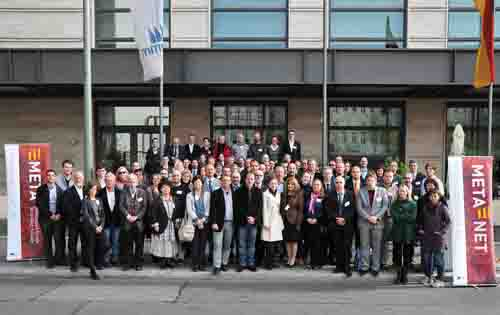
\includegraphics[width=\textwidth]{../_media/meta-net_team.jpg}
  % \fbox{Dummy -- we'll include the group photo of our META-NET meeting in Berlin here}
  \caption{Rinne timpeall 100 saineolaí um theicneolaíocht teanga -- ionadaithe ó na tíortha agus teangacha atá i META-NET -- plé ar phríomhthorthaí agus teachtaireachtaí Shraith Páipéar Bán agus thug siad chun críche iad ag cruinniú i mBeirlín, an Ghearmáin, an 21/22~Deireadh Fómhair 2011. --- \textcolor{grey1}{About 100 language technology experts -- representatives of the countries and languages represented in META-NET -- discussed and finalised the key results and messages of the White Paper Series at a META-NET meeting in Berlin, Germany, on October 21/22, 2011.}} %NEEDS TO BE TRANSLATED
 \medskip
  \colorrule{grey3}{\textwidth}{1.5pt}
\end{figure*}

\cleardoublepage

\bsection[An Sraith Páipéar Bán META-NET -- The META-NET White Paper Series]{An Sraith Páipéar Bán META-NET --- The META-NET\ \ \ \ \ \ White Paper Series}
\label{whitepaperseries}

\vspace*{-5mm}
\centering
  \setlength{\tabcolsep}{2em}
  \begin{tabularx}{\textwidth}{lllll} \toprule\addlinespace
  %\begin{tabulary}{170mm}{LLL} \toprule
  &Bascais & Basque & euskara& \\
  &Béarla & English & English& \\
  &Bokmål Ioruais & Norwegian Bokmål & bokmål& \\
  &Bulgáiris & Bulgarian & български& \\
  &Catalóinis & Catalan & català& \\
  &Cróitis & Croatian & hrvatski& \\
  &Danmhairgis & Danish & dansk& \\
  &Eastóinis & Estonian & eesti& \\
  &Fionlainnis & Finnish & suomi& \\
  &Fraincis & French & français& \\
  &Gailísis & Galician & galego& \\
  &Gaeilge & Irish & Gaeilge& \\
  &Gearmáinis & German & Deutsch& \\
  &Gréigis & Greek & ελληνικά& \\
  &Iodáilis & Italian & italiano& \\
  &Íoslainnis & Icelandic & íslenska& \\
  &Laitvis & Latvian & latviešu valoda& \\
  &Liotuáinis & Lithuanian & lietuviu kalba& \\
  &Máltais & Maltese & Malti& \\
  &Nynorsk Ioruais & Norwegian Nynorsk & nynorsk& \\
  &Ollainnis & Dutch & Nederlands& \\
  &Polainnis & Polish & polski& \\
  &Portaingéilis & Portuguese & português& \\
  &Rómáinis & Romanian & româna& \\
  &Seirbis & Serbian & српски& \\
  &Seicis & Czech & ceština& \\
  &Slóvaicis & Slovak & slovencina& \\
  &Slóivéinis & Slovene & slovenšcina& \\
  &Spáinnis & Spanish & español& \\
  &Sualainnis & Swedish & svenska& \\
  &Ungáiris & Hungarian & magyar& \\ \addlinespace \bottomrule
\end{tabularx} %NEEDS TO BE TRANSLATED

%\end{document}
